%=== Préambule ===========================================================

\documentclass{beamer}
\usepackage{pdfpages}
\usepackage[english]{babel}
\usepackage{xspace}
\usepackage{pifont}
\usepackage{hyperref}
\usepackage{listings}
\usepackage{csquotes}
\usepackage{graphicx}
\usepackage{animate,media9} %,movie15}
\usepackage{wrapfig}
\usepackage{pdfpages}
\usepackage{tikz}
\usepackage{natbib}
\uselanguage{English}
\usepackage{fontawesome5}
\languagepath{English}
\setcounter{tocdepth}{1}
\usepackage{setspace}
\usepackage{amsmath}
\def\glasses{{\sffamily 
\leavevmode\rlap{%
\rotatebox[origin=tr]{125}{J}\kern1ex%  
\rotatebox[origin=tr]{125}{J}}% 
\rotatebox[origin=c]{-90}{D}%   
\rotatebox[origin=c]{-90}{D}}%
\def\ialy{\sffamily 
\resizebox{1ex}{1.5ex}{\reflectbox{\rotatebox[origin=]{75}{J}}}\kern-1pt%
\rlap{\tiny$\ ^\bullet\kern2.5pt^\bullet$ }%
\rotatebox[origin=c]{-90}{D}%   
\rotatebox[origin=c]{-90}{D}\kern-1pt%  
\resizebox{1ex}{1.5ex}{\rotatebox[origin=]{75}{J}}}}


\lstset{
  numbers=left,
  basicstyle=\tiny\ttfamily,      
  breaklines=true, 
  showtabs=false,
  showstringspaces=false,
}  

%=== Configuration de Beamer et du thème metropolis ======================
\usepackage{bbding}
\usetheme[background=light]{metropolis}
\usepackage[clock]{ifsym}

\definecolor{mLightBrown}{HTML}{000000}
\definecolor{black}{HTML}{000000}
\setbeamercolor{structure}{fg=black,bg=mLightBrown}
\setbeamercolor{palette primary}{%
	use=normal text,
	fg=normal text.bg,
	bg=mLightBrown
}
%\setsansfont[BoldFont={Linux Libertine G Bold},Numbers={OldStyle}]{Linux Libertine G}

\metroset{block=fill}

%=== Page de titre =======================================================

%path to logo and biblio -> to be adapted to your local directories 
\newcommand\dirlogo{../../logos/}
\newcommand\dirbiblio{../../biblio}



\title{{\normalsize \vskip 1cm Exploring complex normal faulting systems through physics-based dynamic rupture modeling}}
\subtitle{\small Cycle Team Meeting}
\author{Hugo S. \\ {\tiny Institut de Recherche pour le Développement IRD - ISTerre} \\ 
\\
O., Scotti, S., Hok, A.-A. Gabriel and T. Taufiqurrahman \\
\\
\textit{ANR EQTIME Project}
}


\date[2021]{\today}

\subject{Group Meeting}

\titlegraphic{\centering \vspace{-15pt}
\includegraphics[height=1.3cm]{../../logos/logo_all_presentation.pdf} \par} %\qquad  
\includegraphics[height=1.4cm]{../../logos/anr_eqtime.png} \par }


\addtobeamertemplate{frametitle}{}{%
\begin{tikzpicture}[remember picture,overlay]
  \node[anchor=north east,yshift=0.0ex] at (current page.north east) {
\includegraphics[height=4ex]{../../logos/ISTerre_neg.pdf}};
  %\node[anchor=north east,yshift=0.5ex] at (current page.north east) {\includegraphics[height=3.3ex]{\dirlogo/seiscope_color_light_background}};
\end{tikzpicture}}



%=== Document ============================================================

\begin{document}

% --- Préambule ---------------------------------------------------------------

\begin{frame}
    \titlepage
\end{frame}

\begin{frame}
 {Outline}
 
 \tableofcontents
 
\end{frame}


\begin{frame}
 {My skills}
 
 \begin{itemize}
  \item Static \& Kinematic coseismic modeling/inversion \pause
  \\
  \item Monitoring seismic activity \pause
  \\
  \item Dynamic seismic source modeling
 \end{itemize}

 
\end{frame}


\begin{frame}
 {My skills}
 
 \begin{itemize}
  \item Static \& Kinematic coseismic modeling/inversion
  \\
  \item Monitoring seismic activity
  \\
  \item \underline{\bf Dynamic seismic source modeling}
 \end{itemize}
 
\end{frame}


\section{Motivation}


\begin{frame}
 {Seismic Hazard in Central Italy}
 
 \begin{center}
  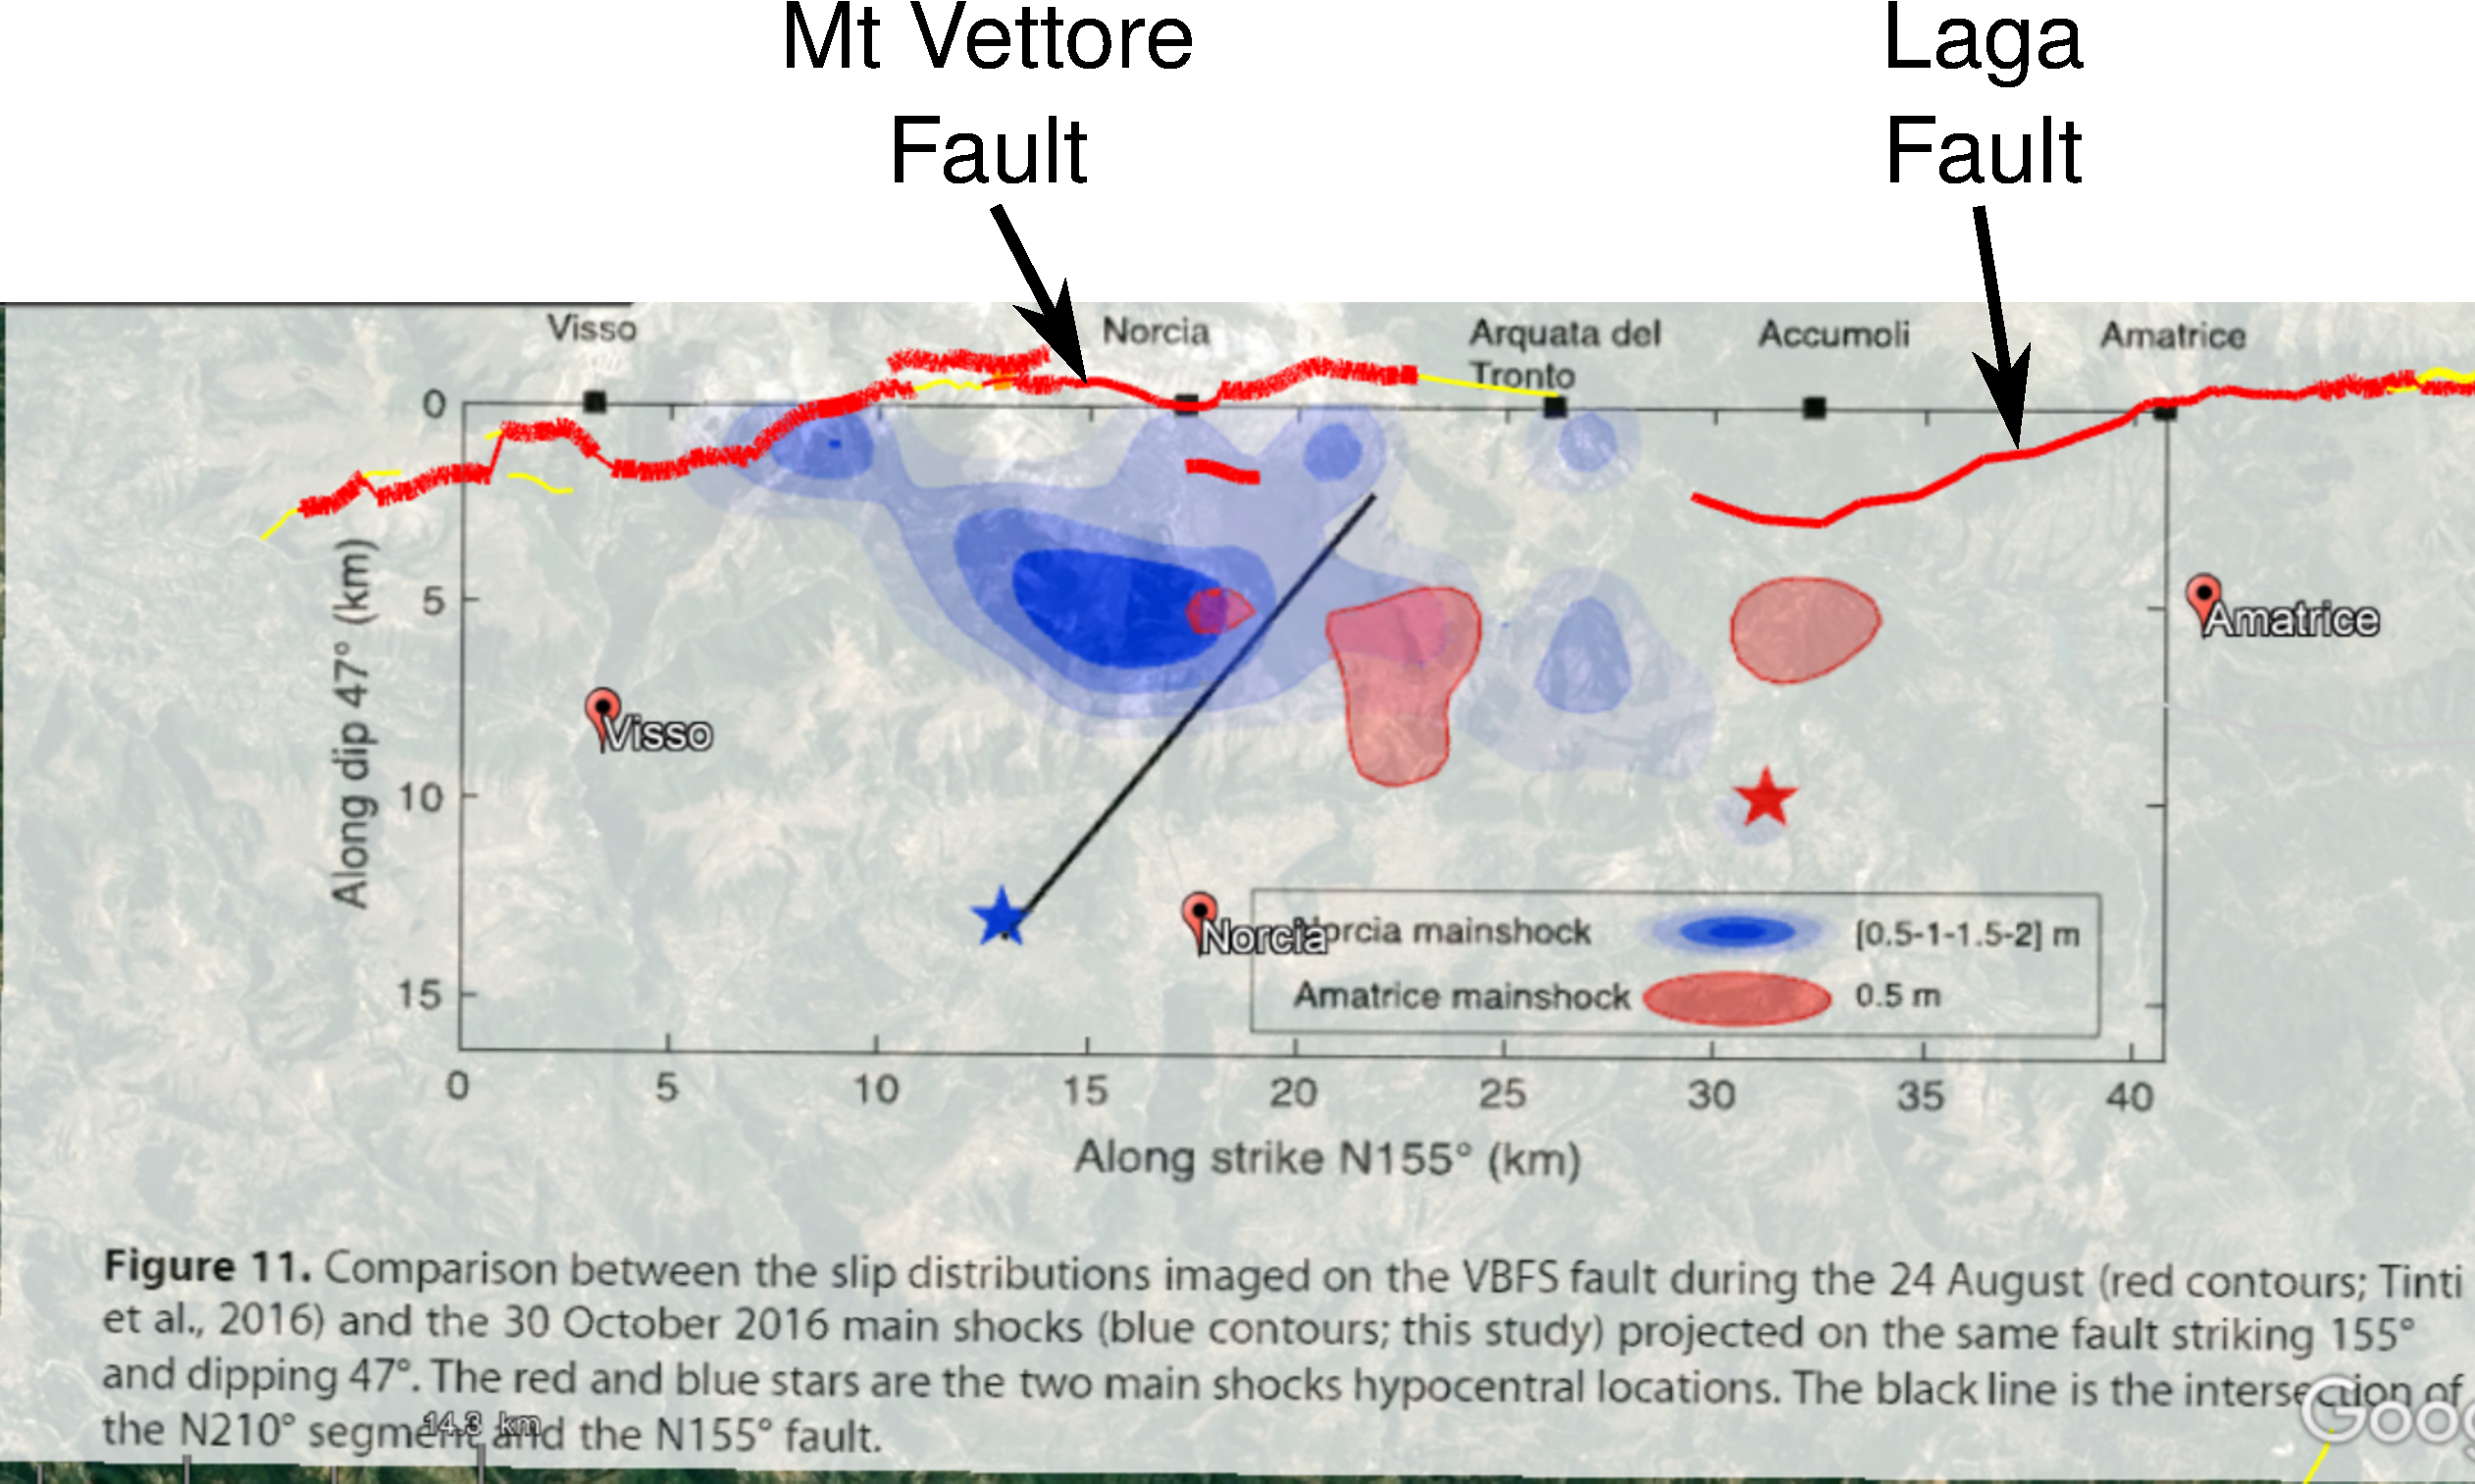
\includegraphics[width=0.65\linewidth]{images/amatrice_1.pdf} \,
  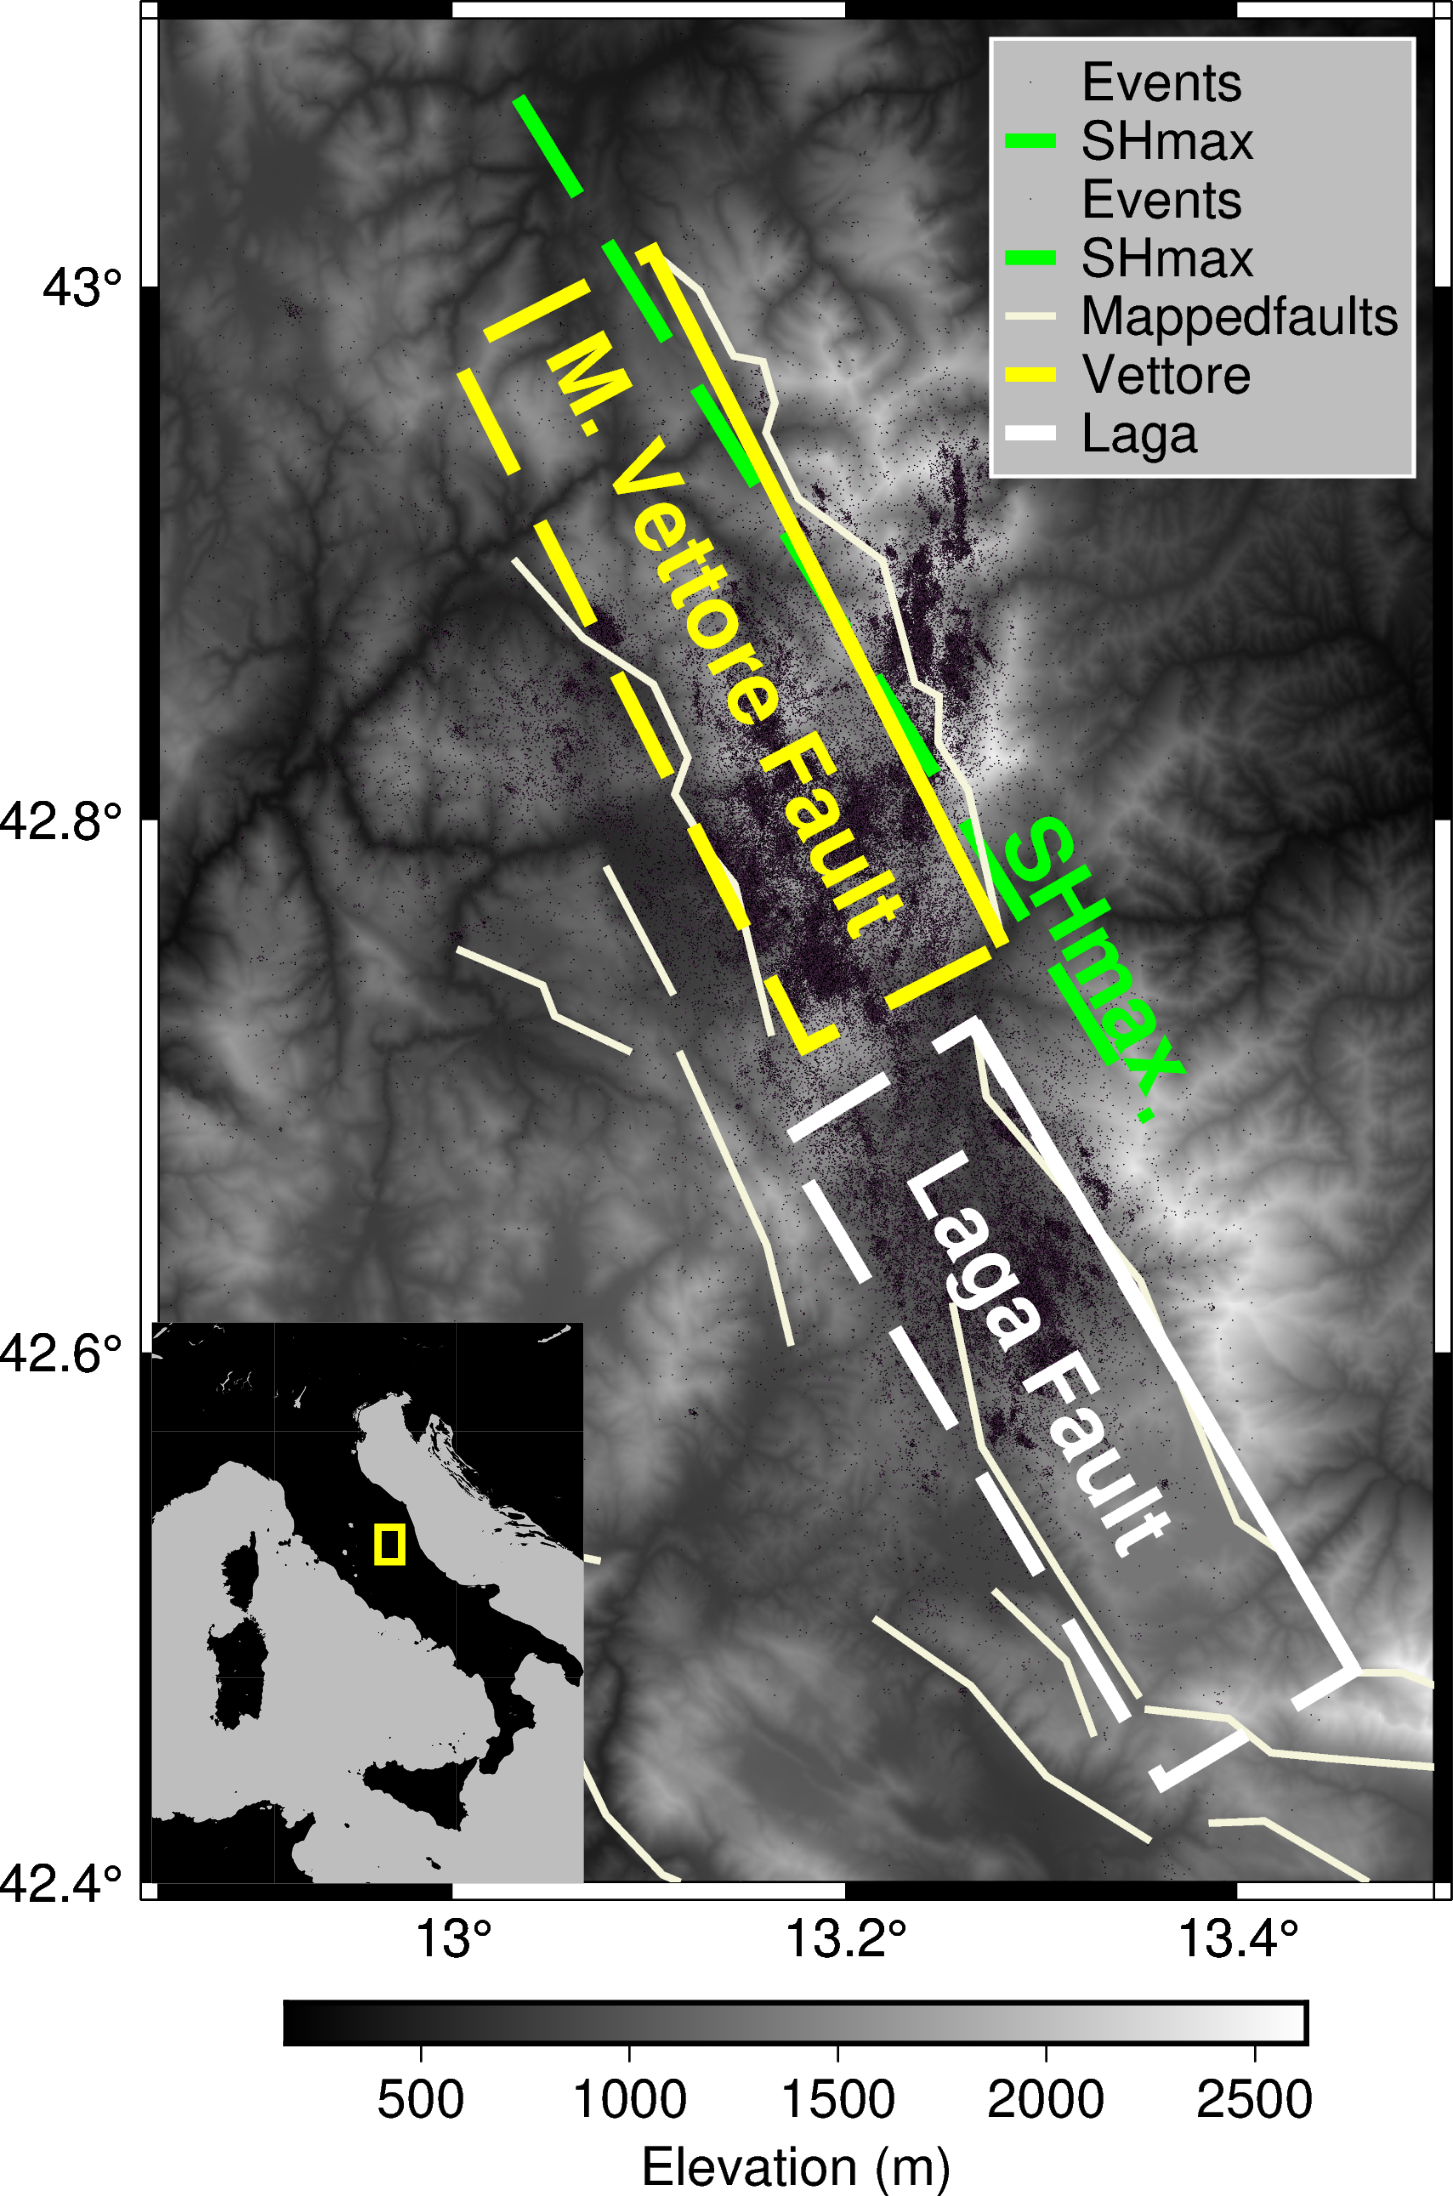
\includegraphics[width=0.3\linewidth]{images/map_italy.png}  
 \end{center}
  \vskip 0.2cm
  {\bf \hfill \scriptsize Modified by O. Scotti from \cite{Scognamiglio_2018_CFG}}
  
\end{frame}

\begin{frame}
 {Seismic Hazard in Central Italy}
 
 \begin{center}
    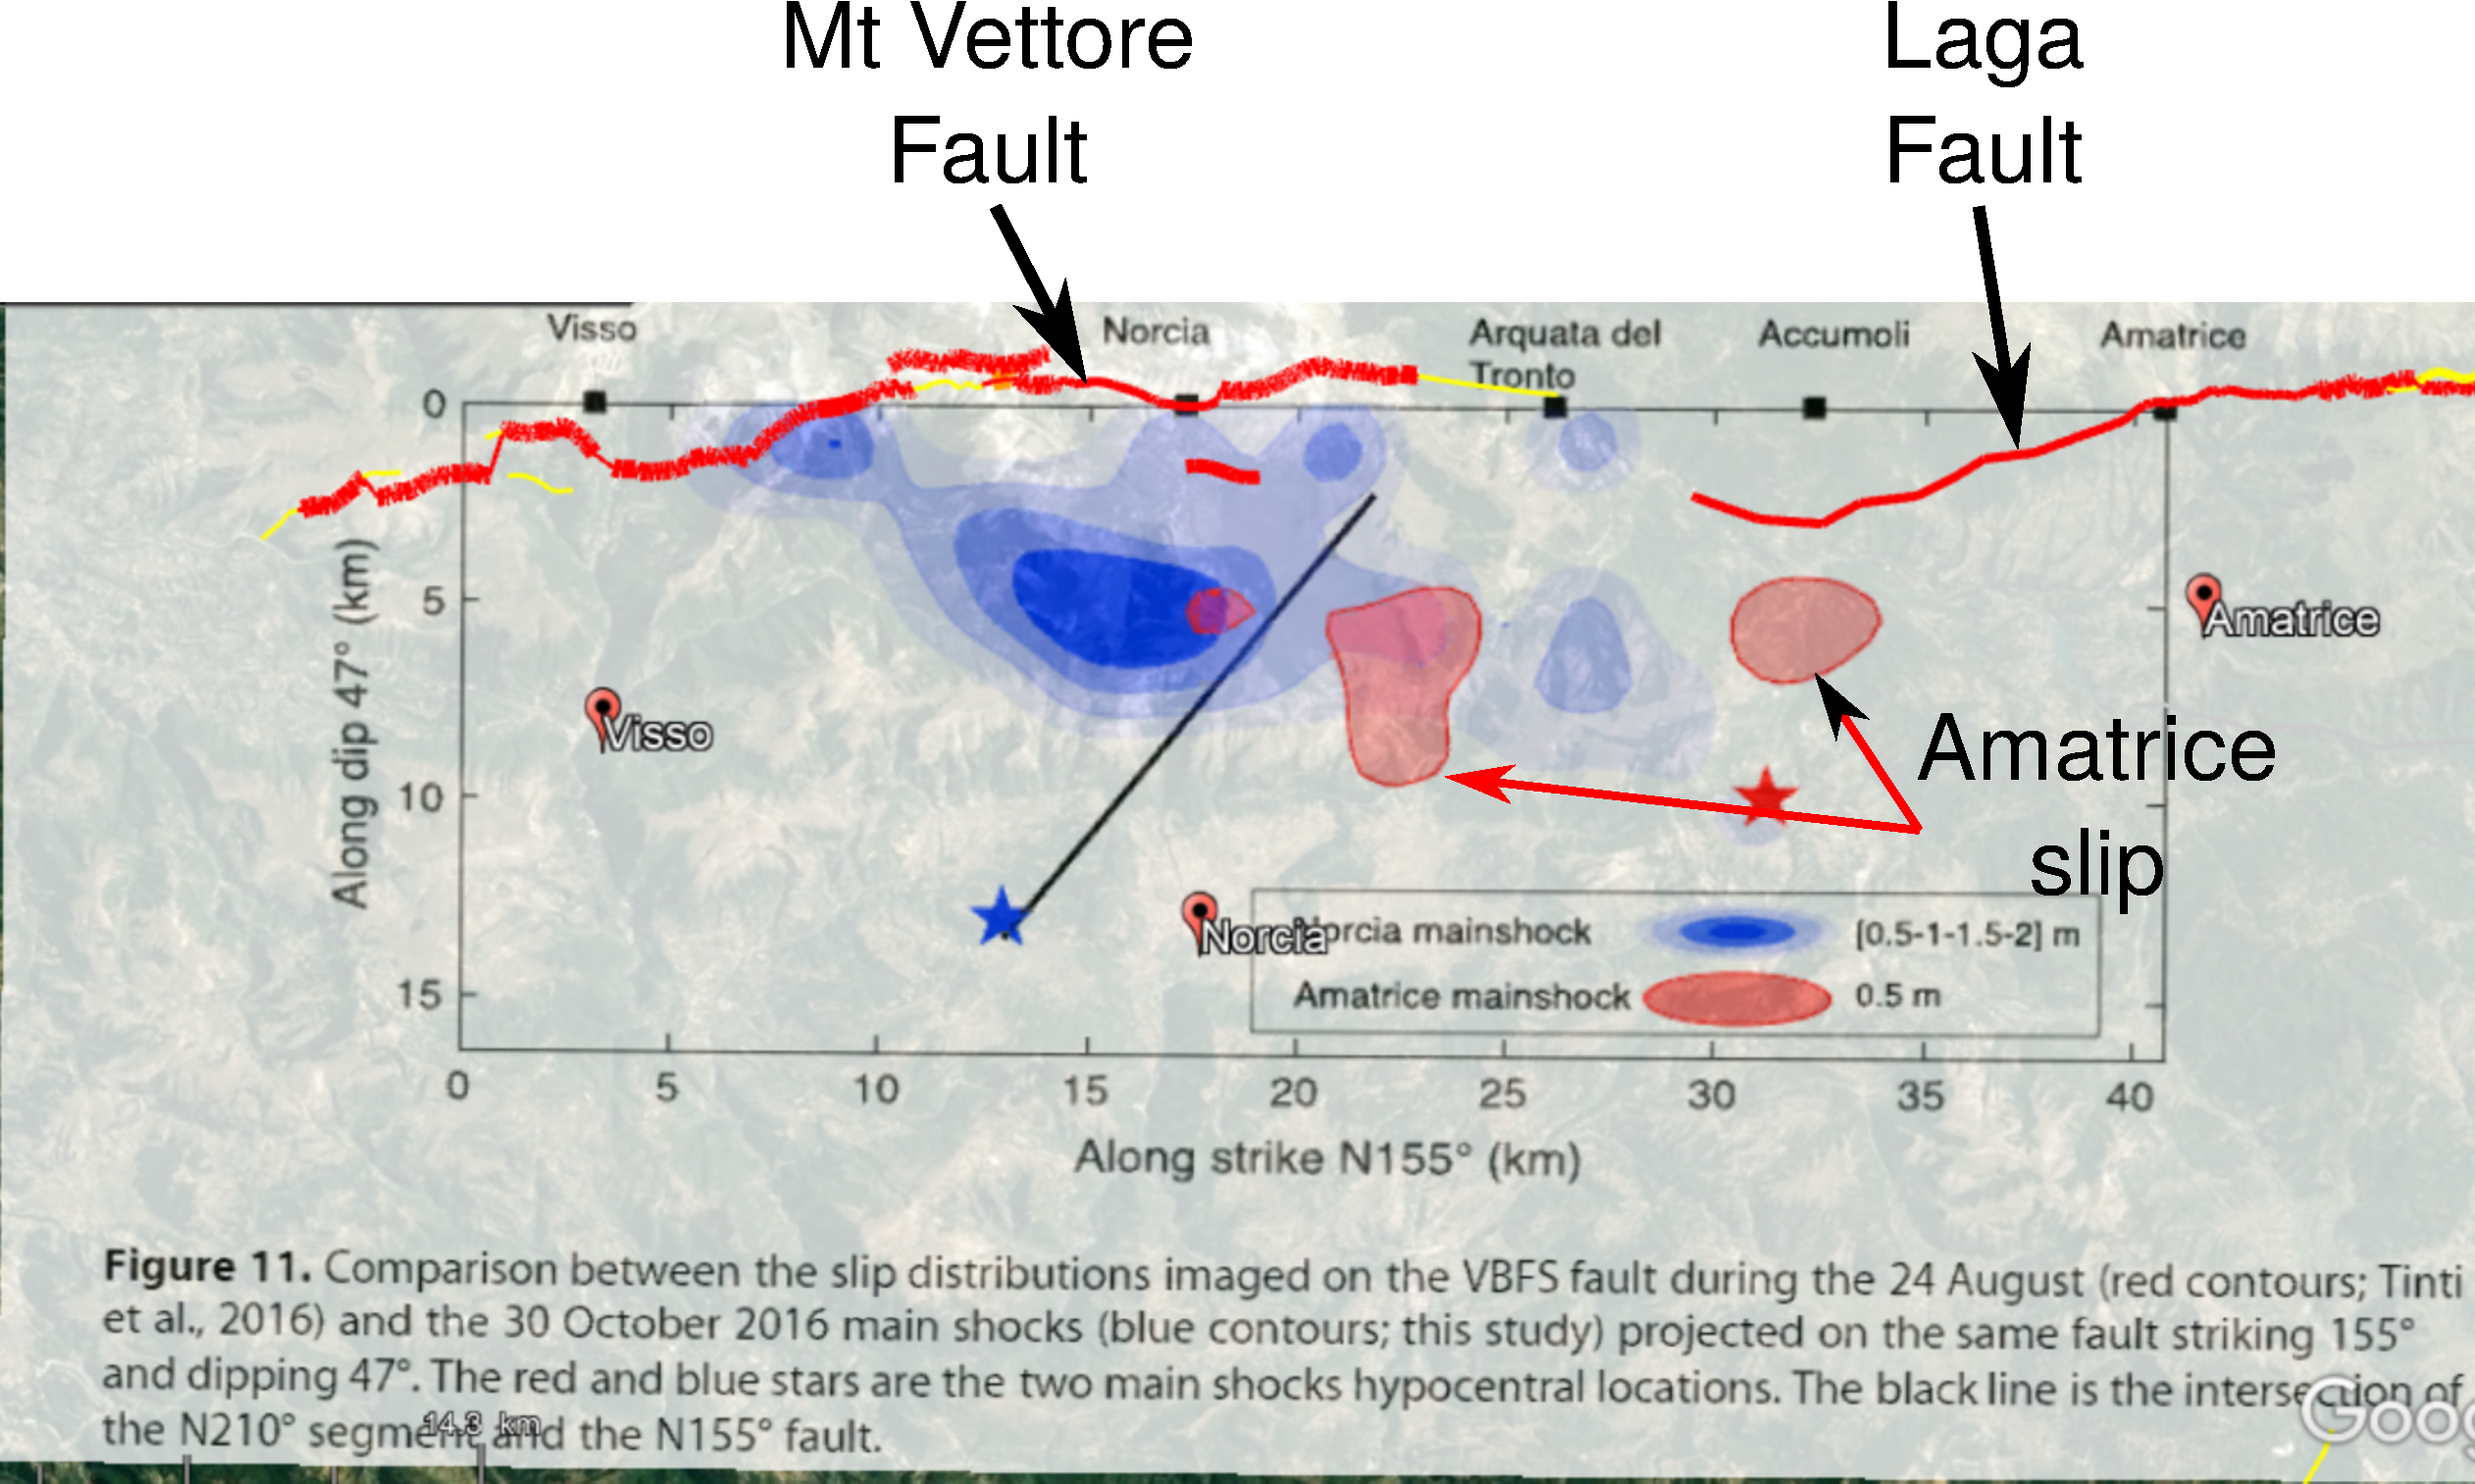
\includegraphics[width=0.65\linewidth]{images/amatrice_2.pdf} \,
    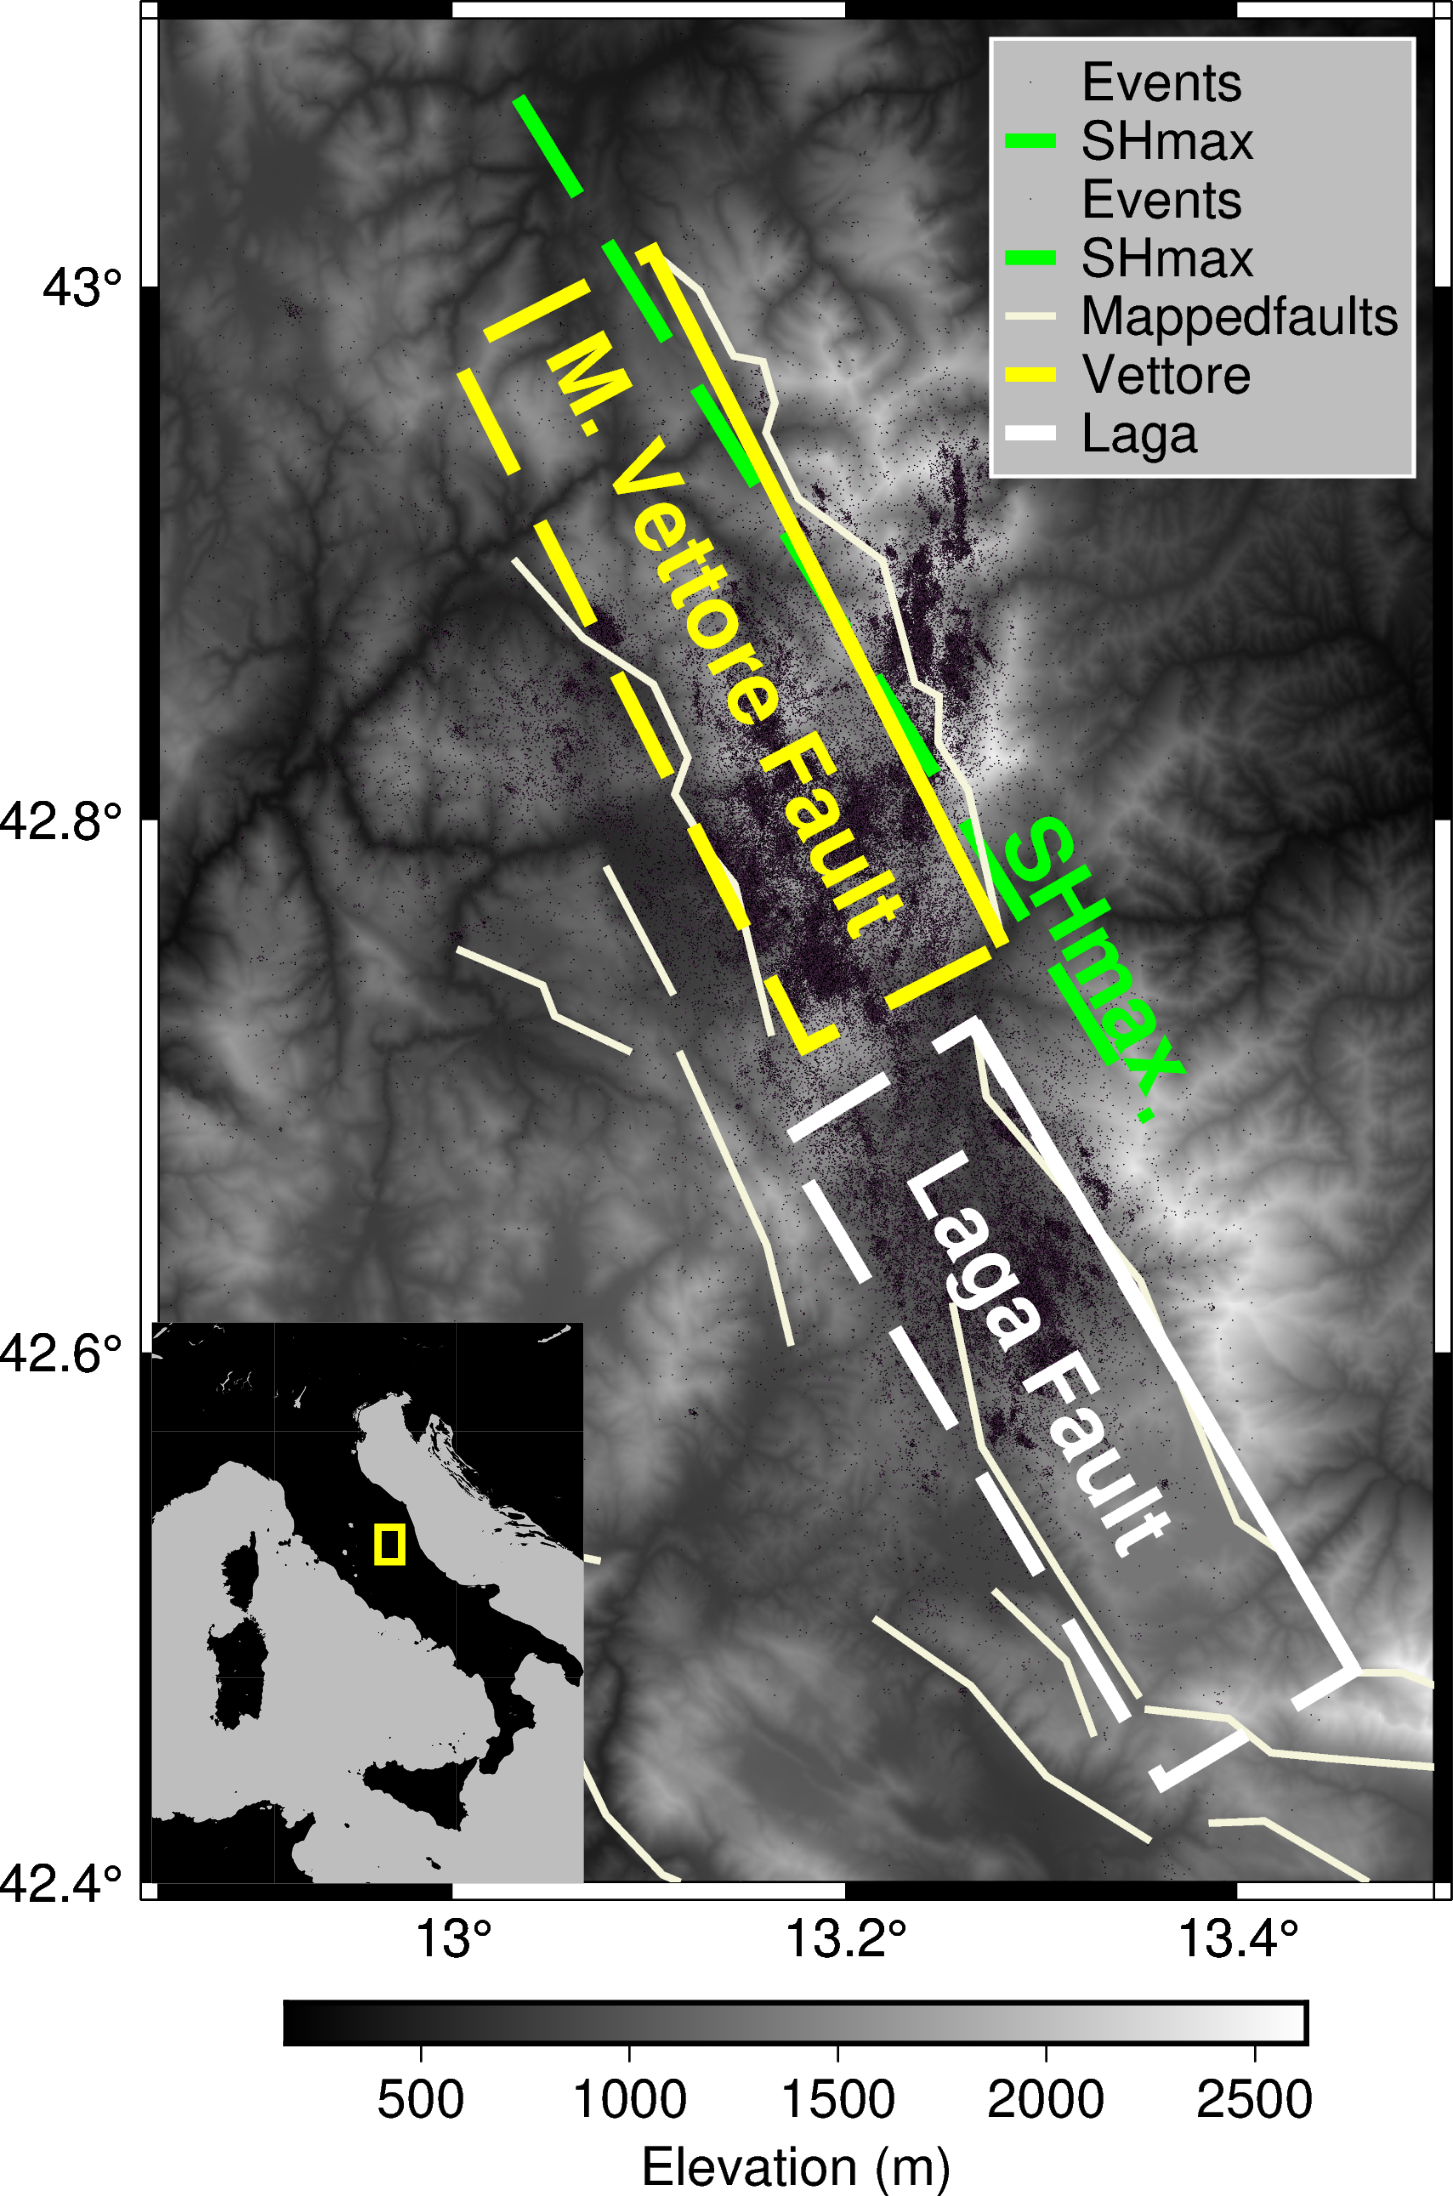
\includegraphics[width=0.3\linewidth]{images/map_italy.png}  
 \end{center}
  \vskip 0.2cm
  {\bf \hfill \scriptsize Modified by O. Scotti from \cite{Scognamiglio_2018_CFG}}
  \addtocounter{framenumber}{-1}
  
\end{frame}


\begin{frame}
 {Seismic Hazard in Central Italy}

 \begin{center}
  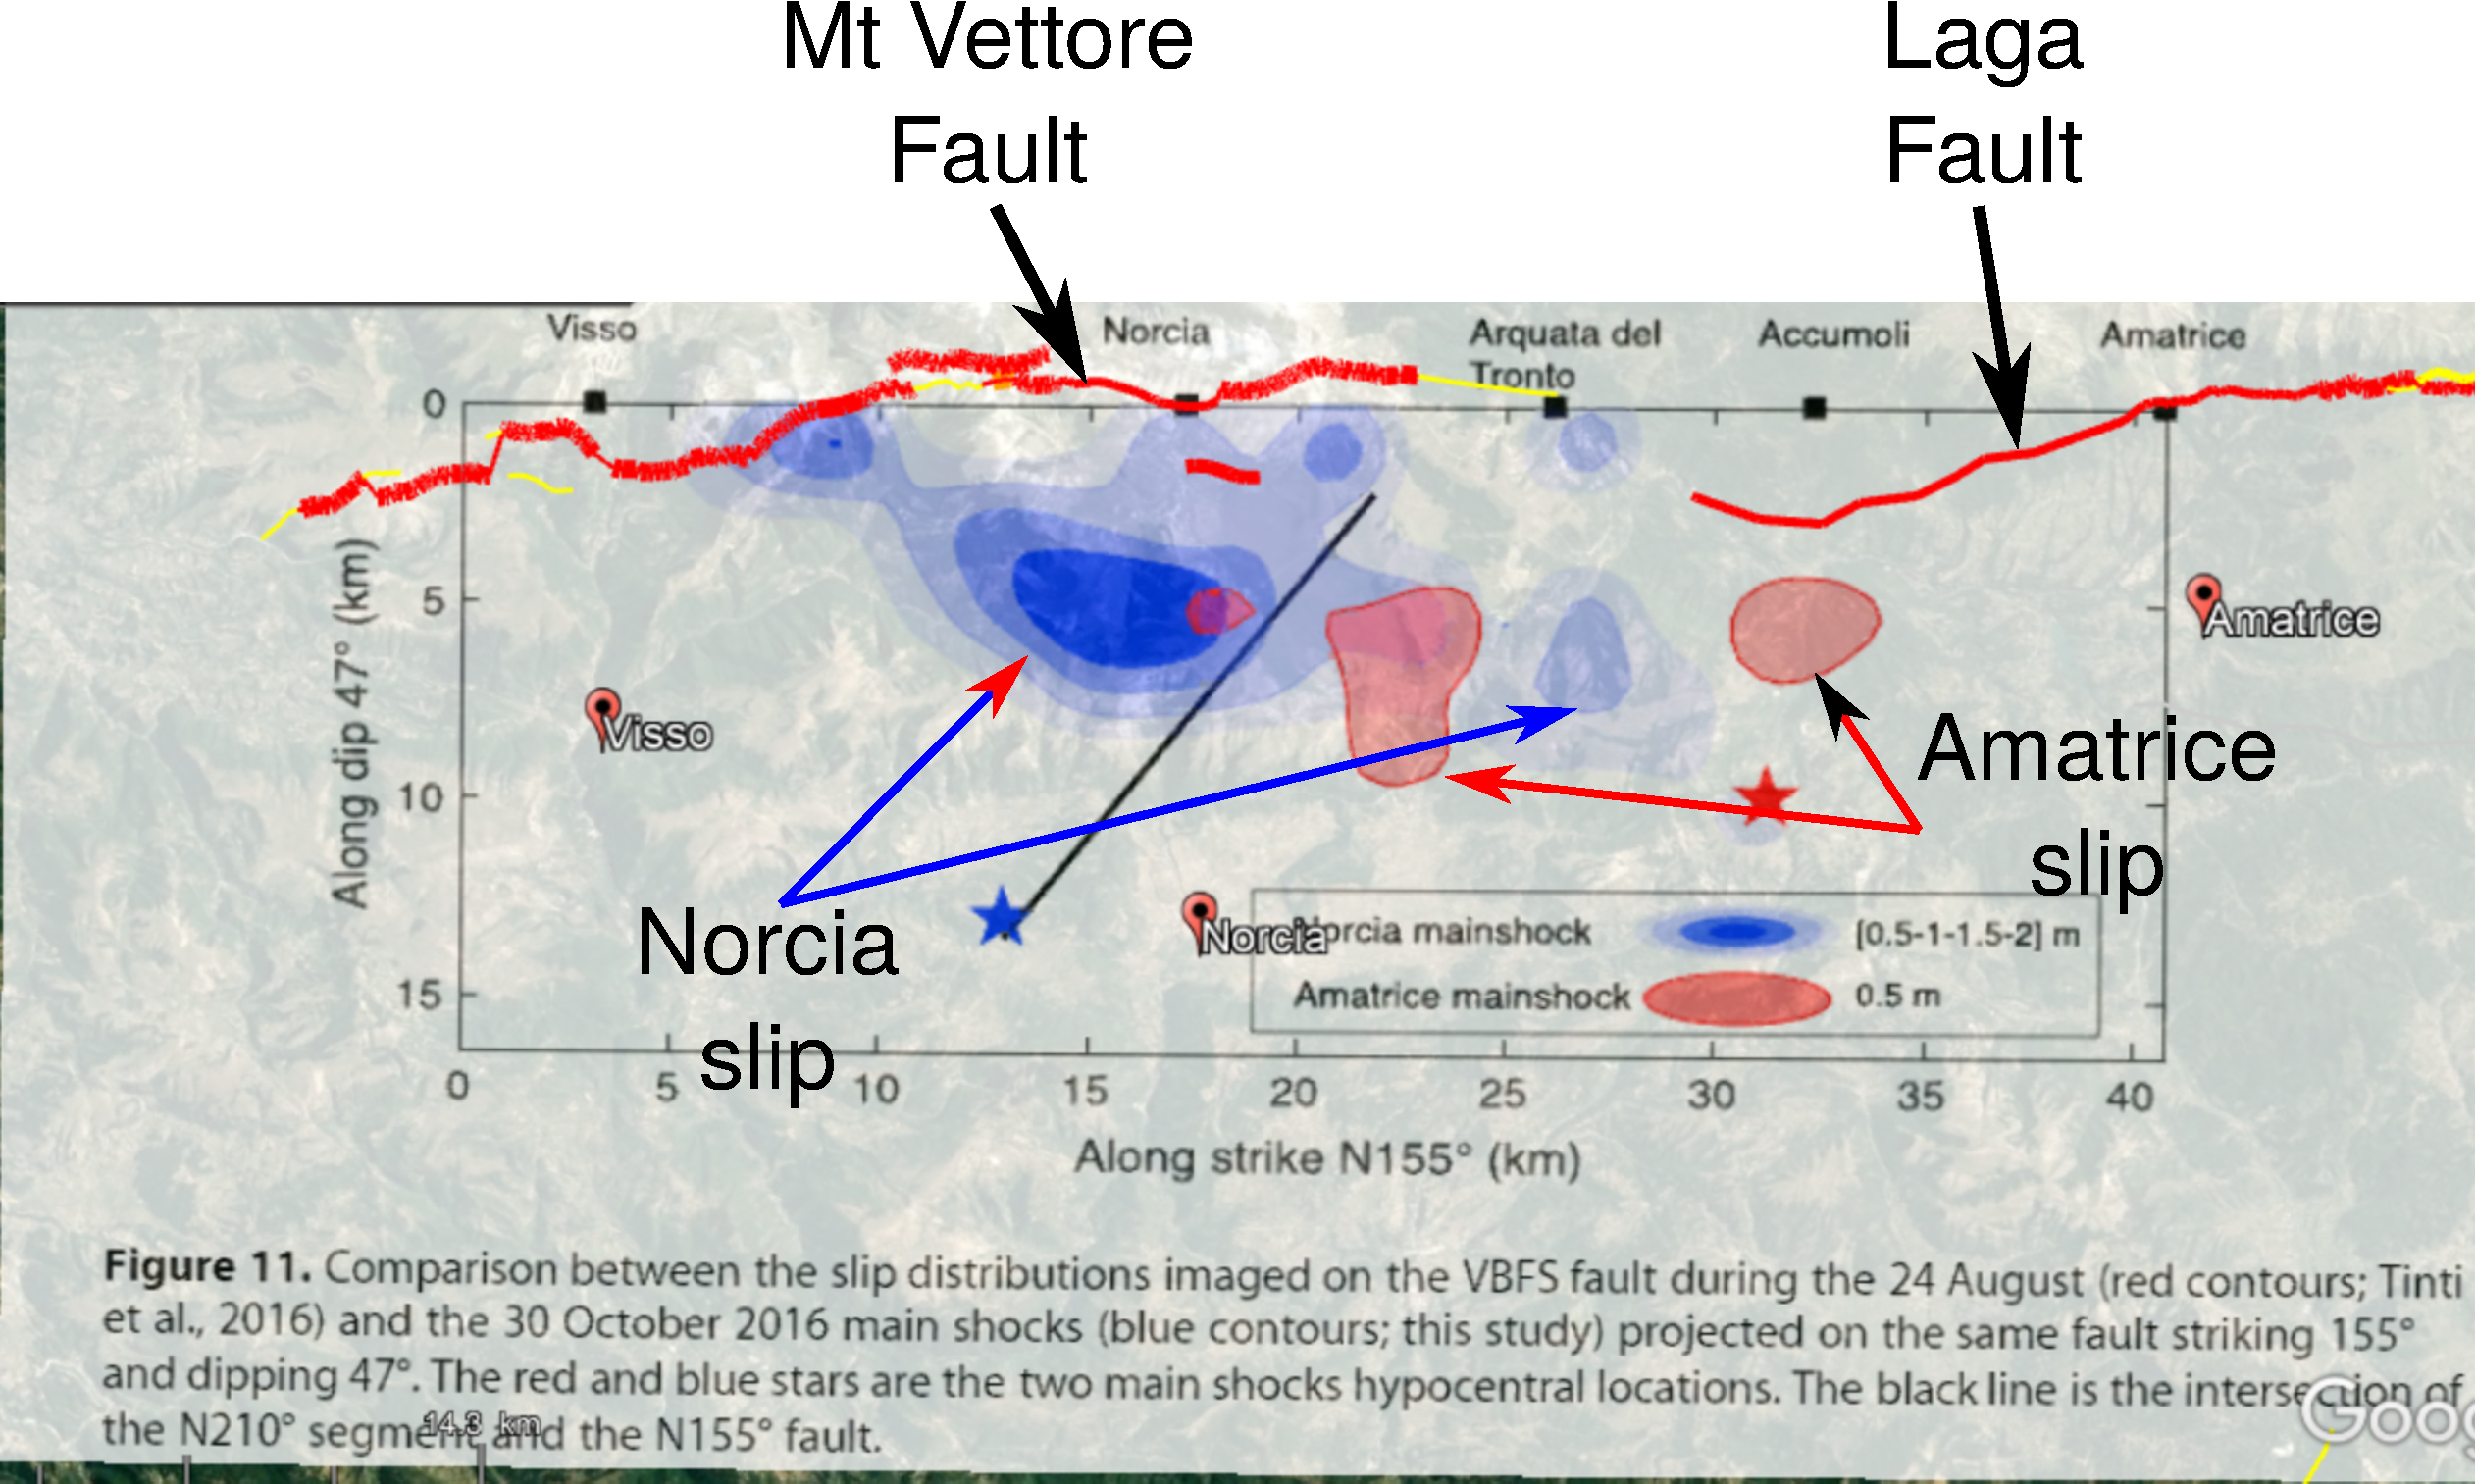
\includegraphics[width=0.65\linewidth]{images/amatrice_3.pdf} \,
  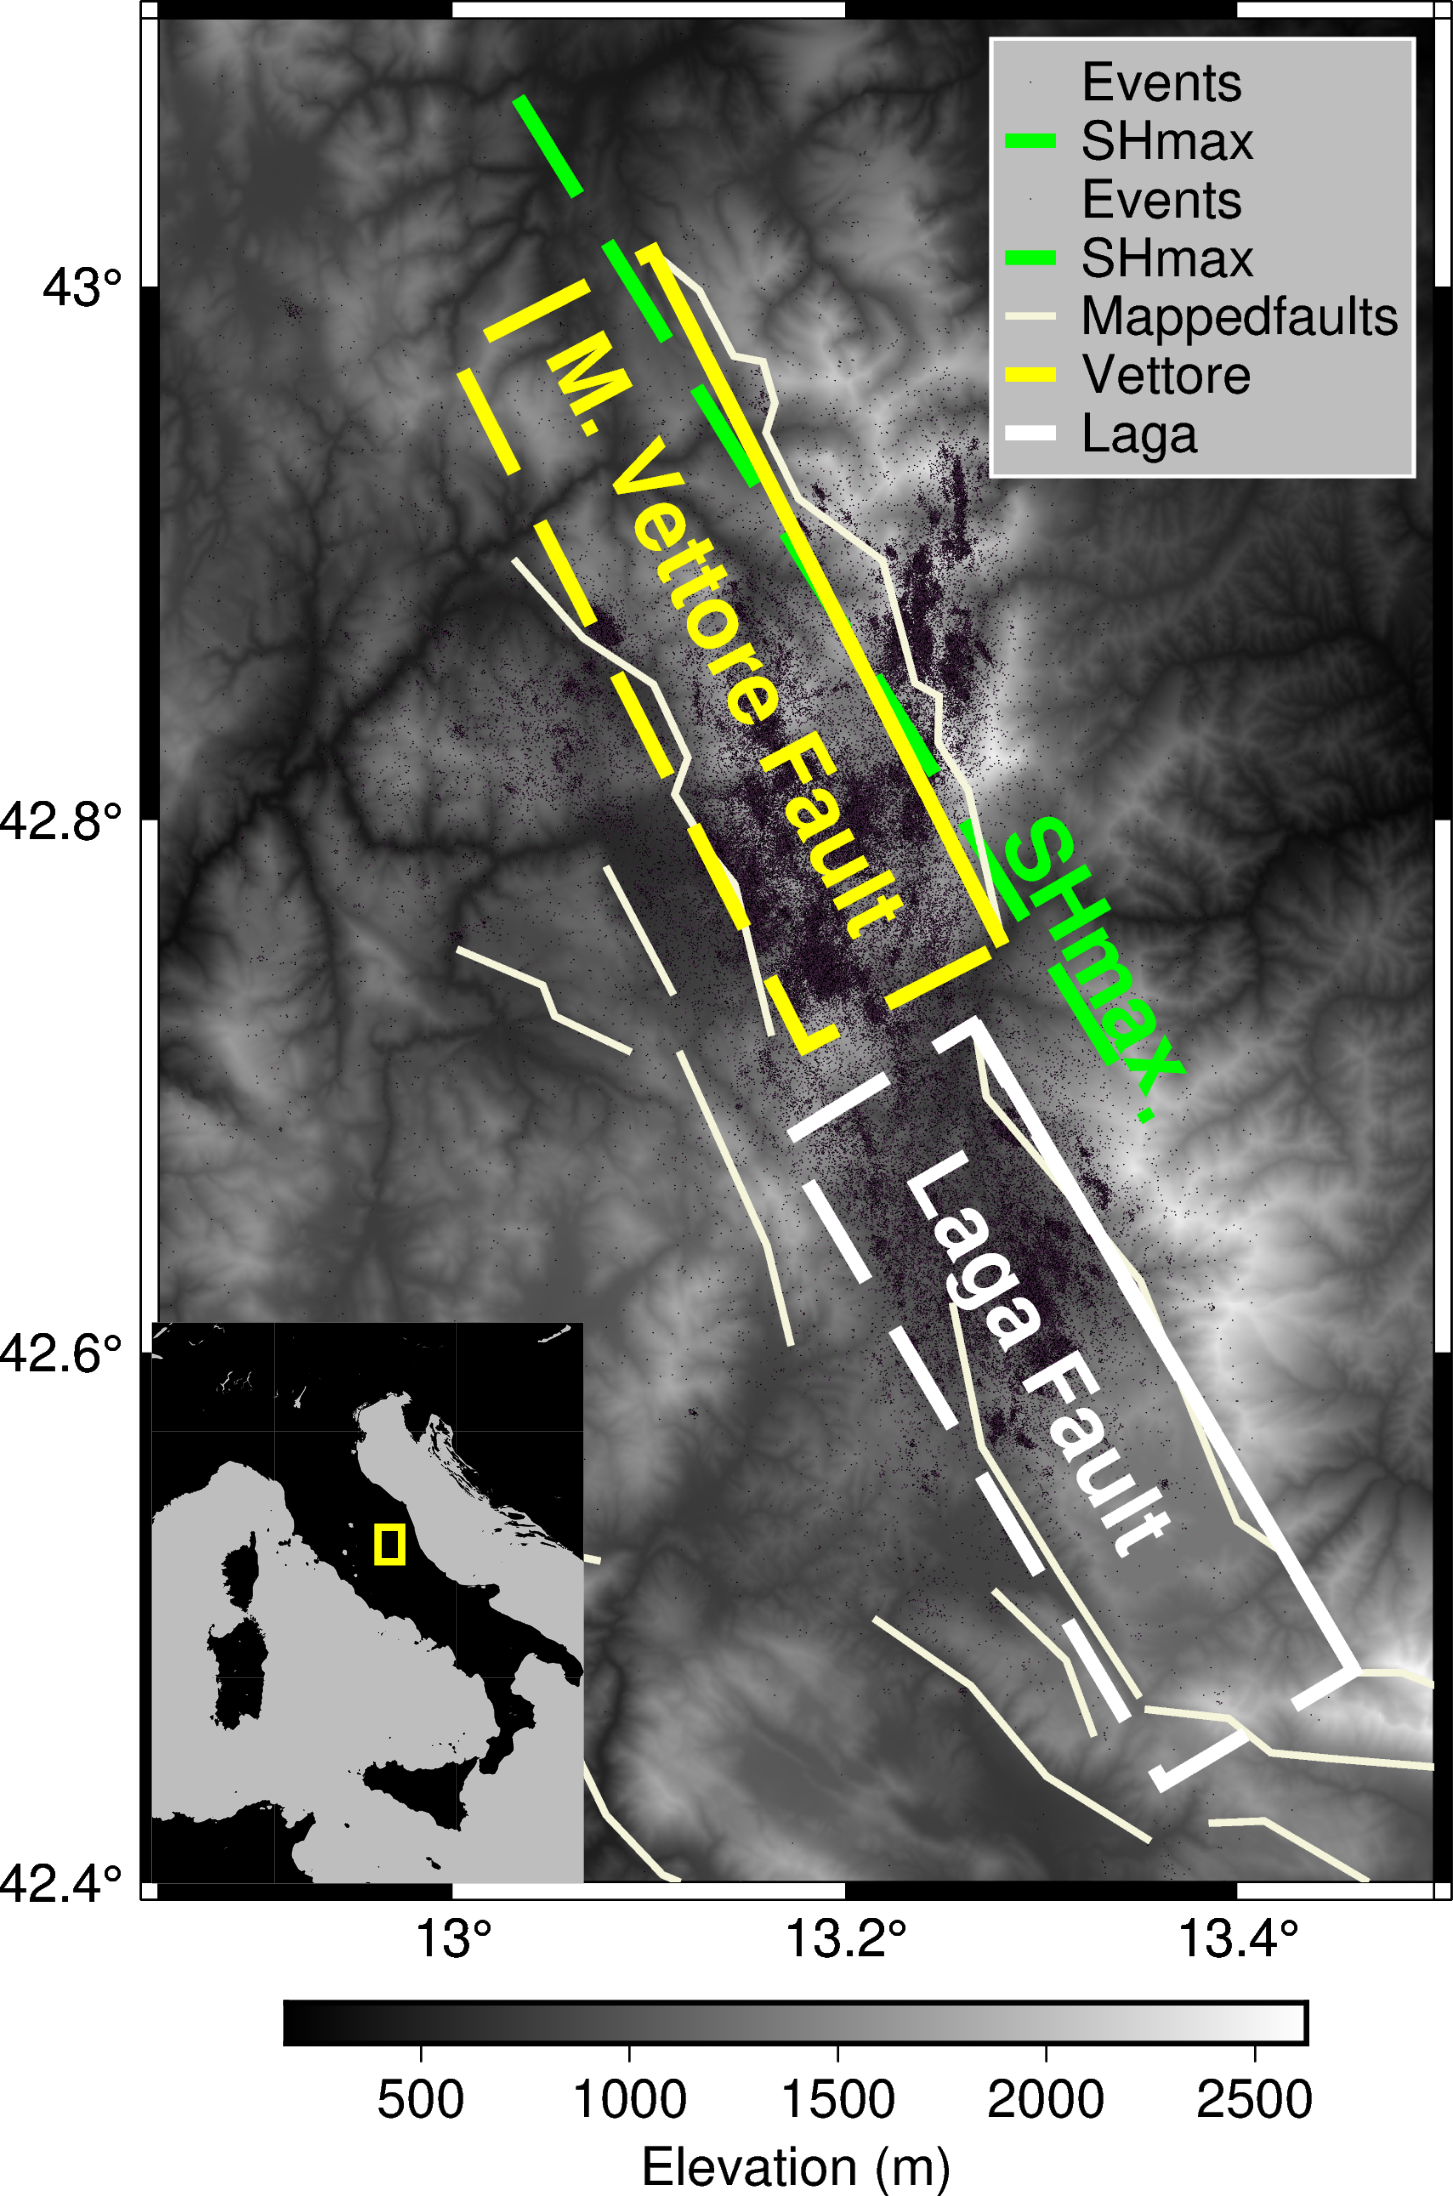
\includegraphics[width=0.3\linewidth]{images/map_italy.png}  
 \end{center}
  \vskip 0.2cm
  {\bf \hfill \scriptsize Modified by O. Scotti from \cite{Scognamiglio_2018_CFG}}
  \addtocounter{framenumber}{-1}
  
\end{frame}


\begin{frame}
 {Seismic Hazard in Central Italy}
 
 \begin{center}
  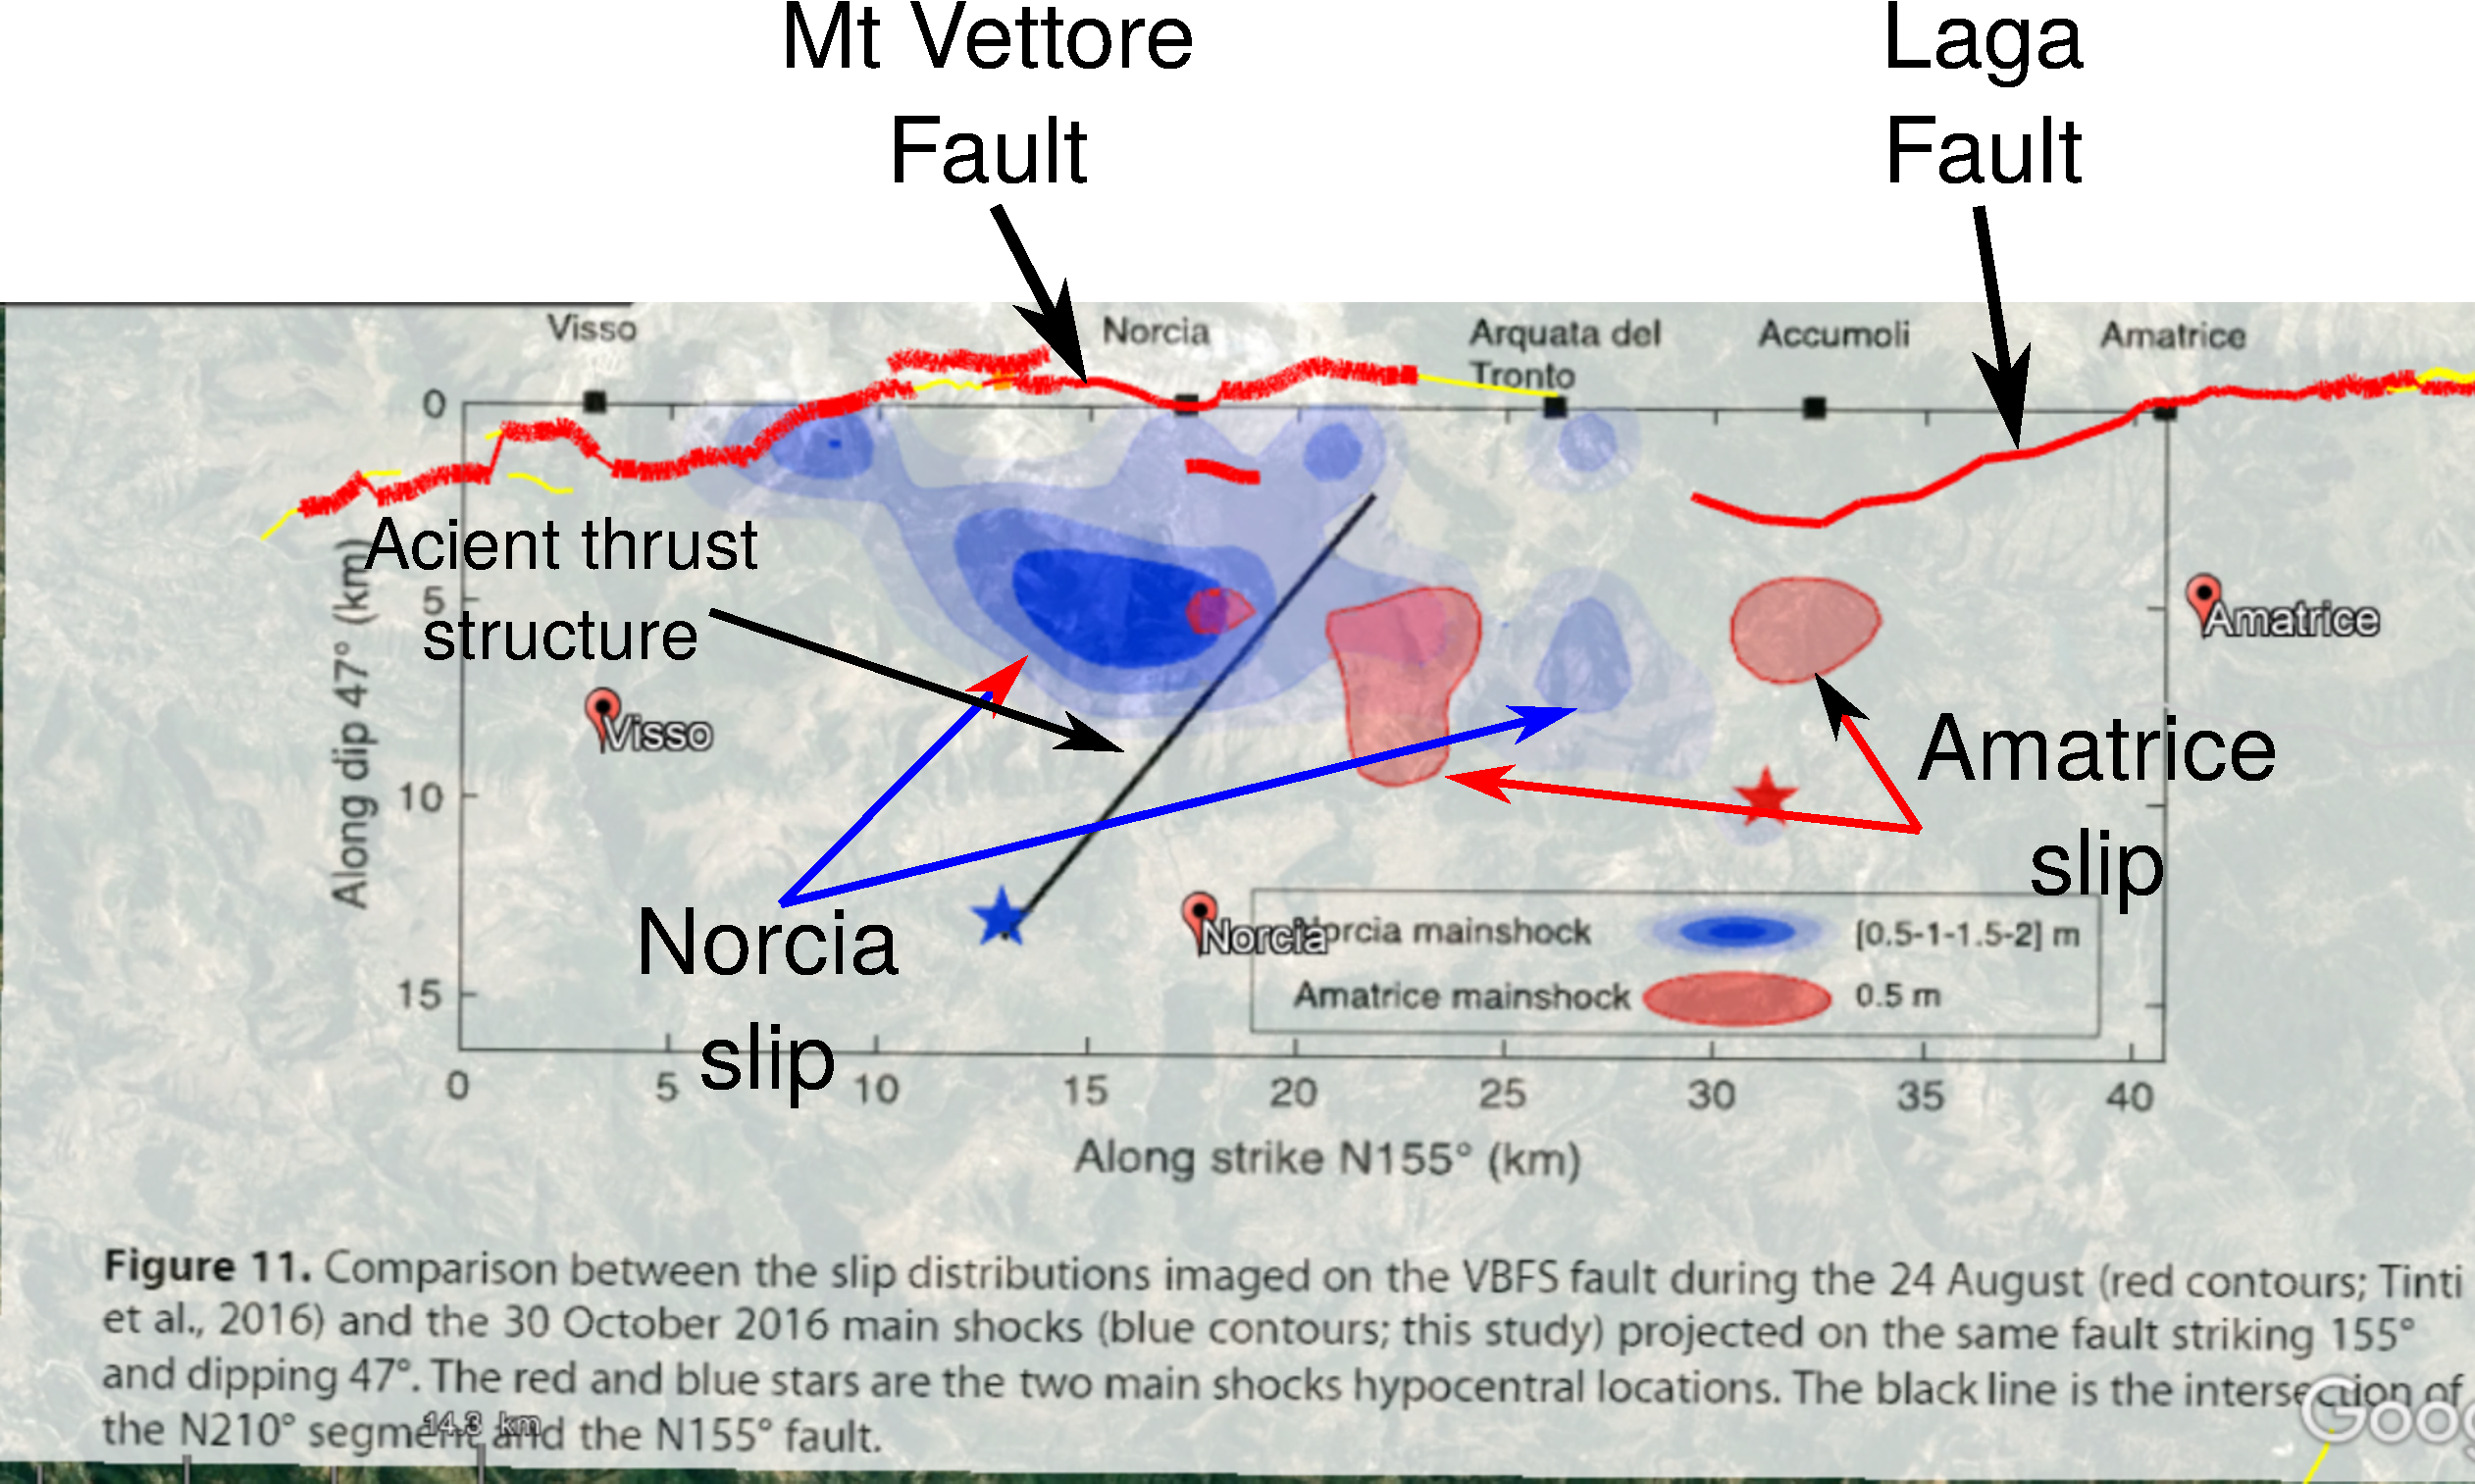
\includegraphics[width=0.65\linewidth]{images/amatrice_4.pdf} \,
  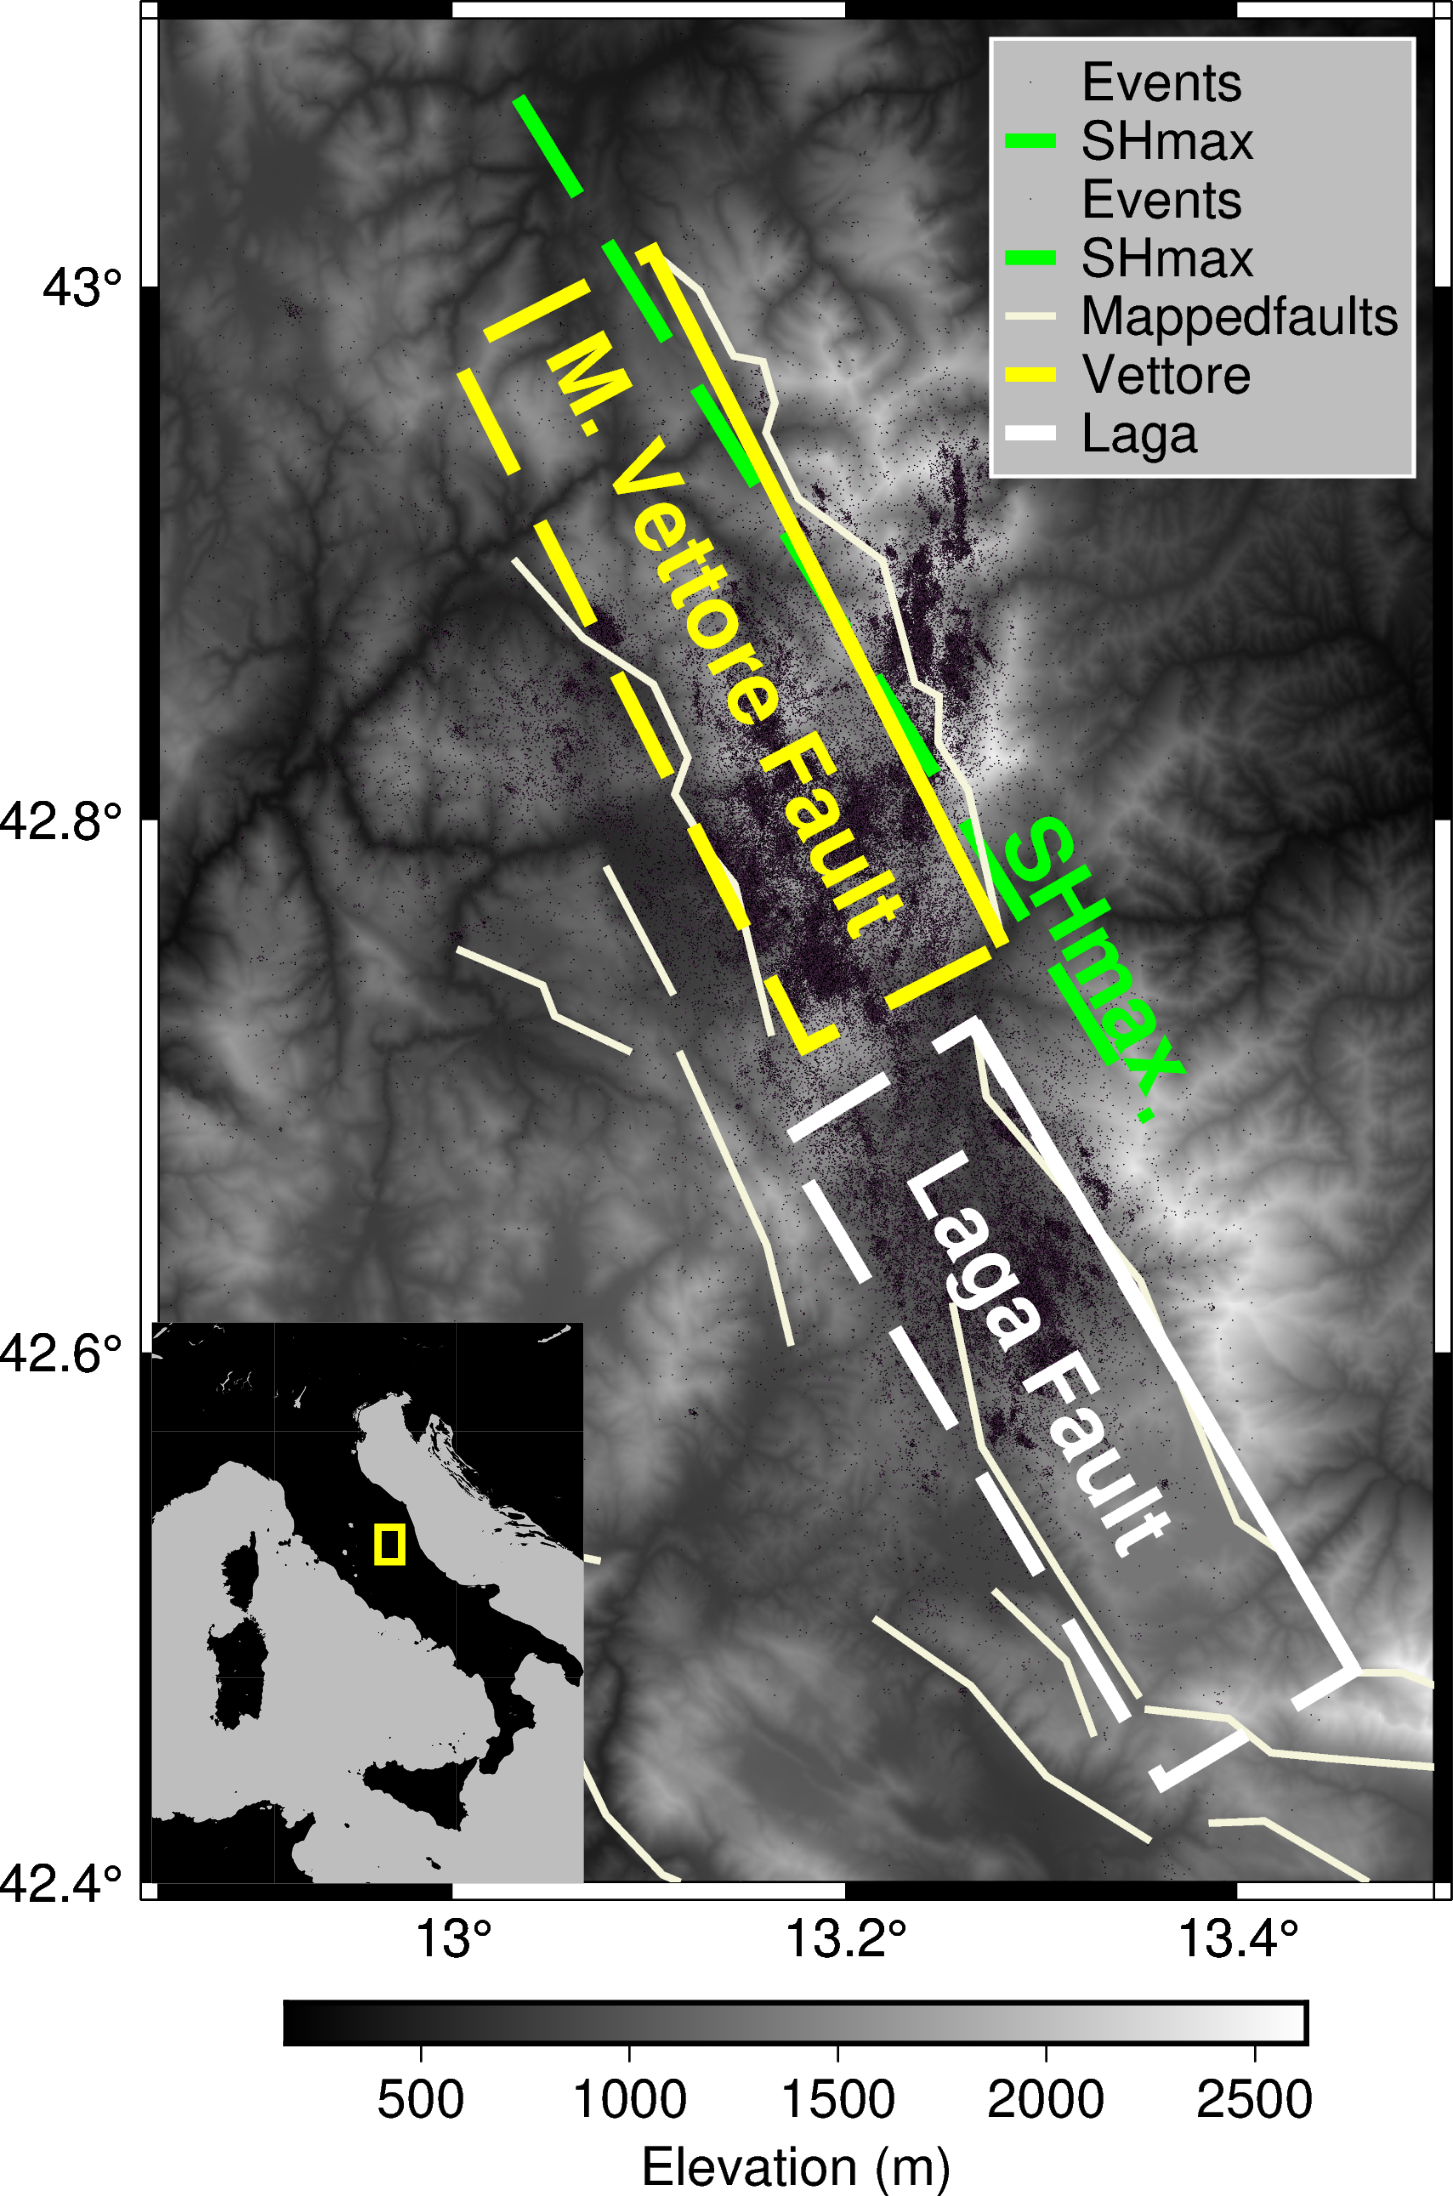
\includegraphics[width=0.3\linewidth]{images/map_italy.png}  
 \end{center}

  \vskip 0.2cm
  {\bf \hfill \scriptsize Modified by O. Scotti from \cite{Scognamiglio_2018_CFG}}
  \addtocounter{framenumber}{-1}
  
\end{frame}


\begin{frame}
 {Seismic Hazard in Central Italy}
 
 \begin{minipage}{0.45\linewidth}
  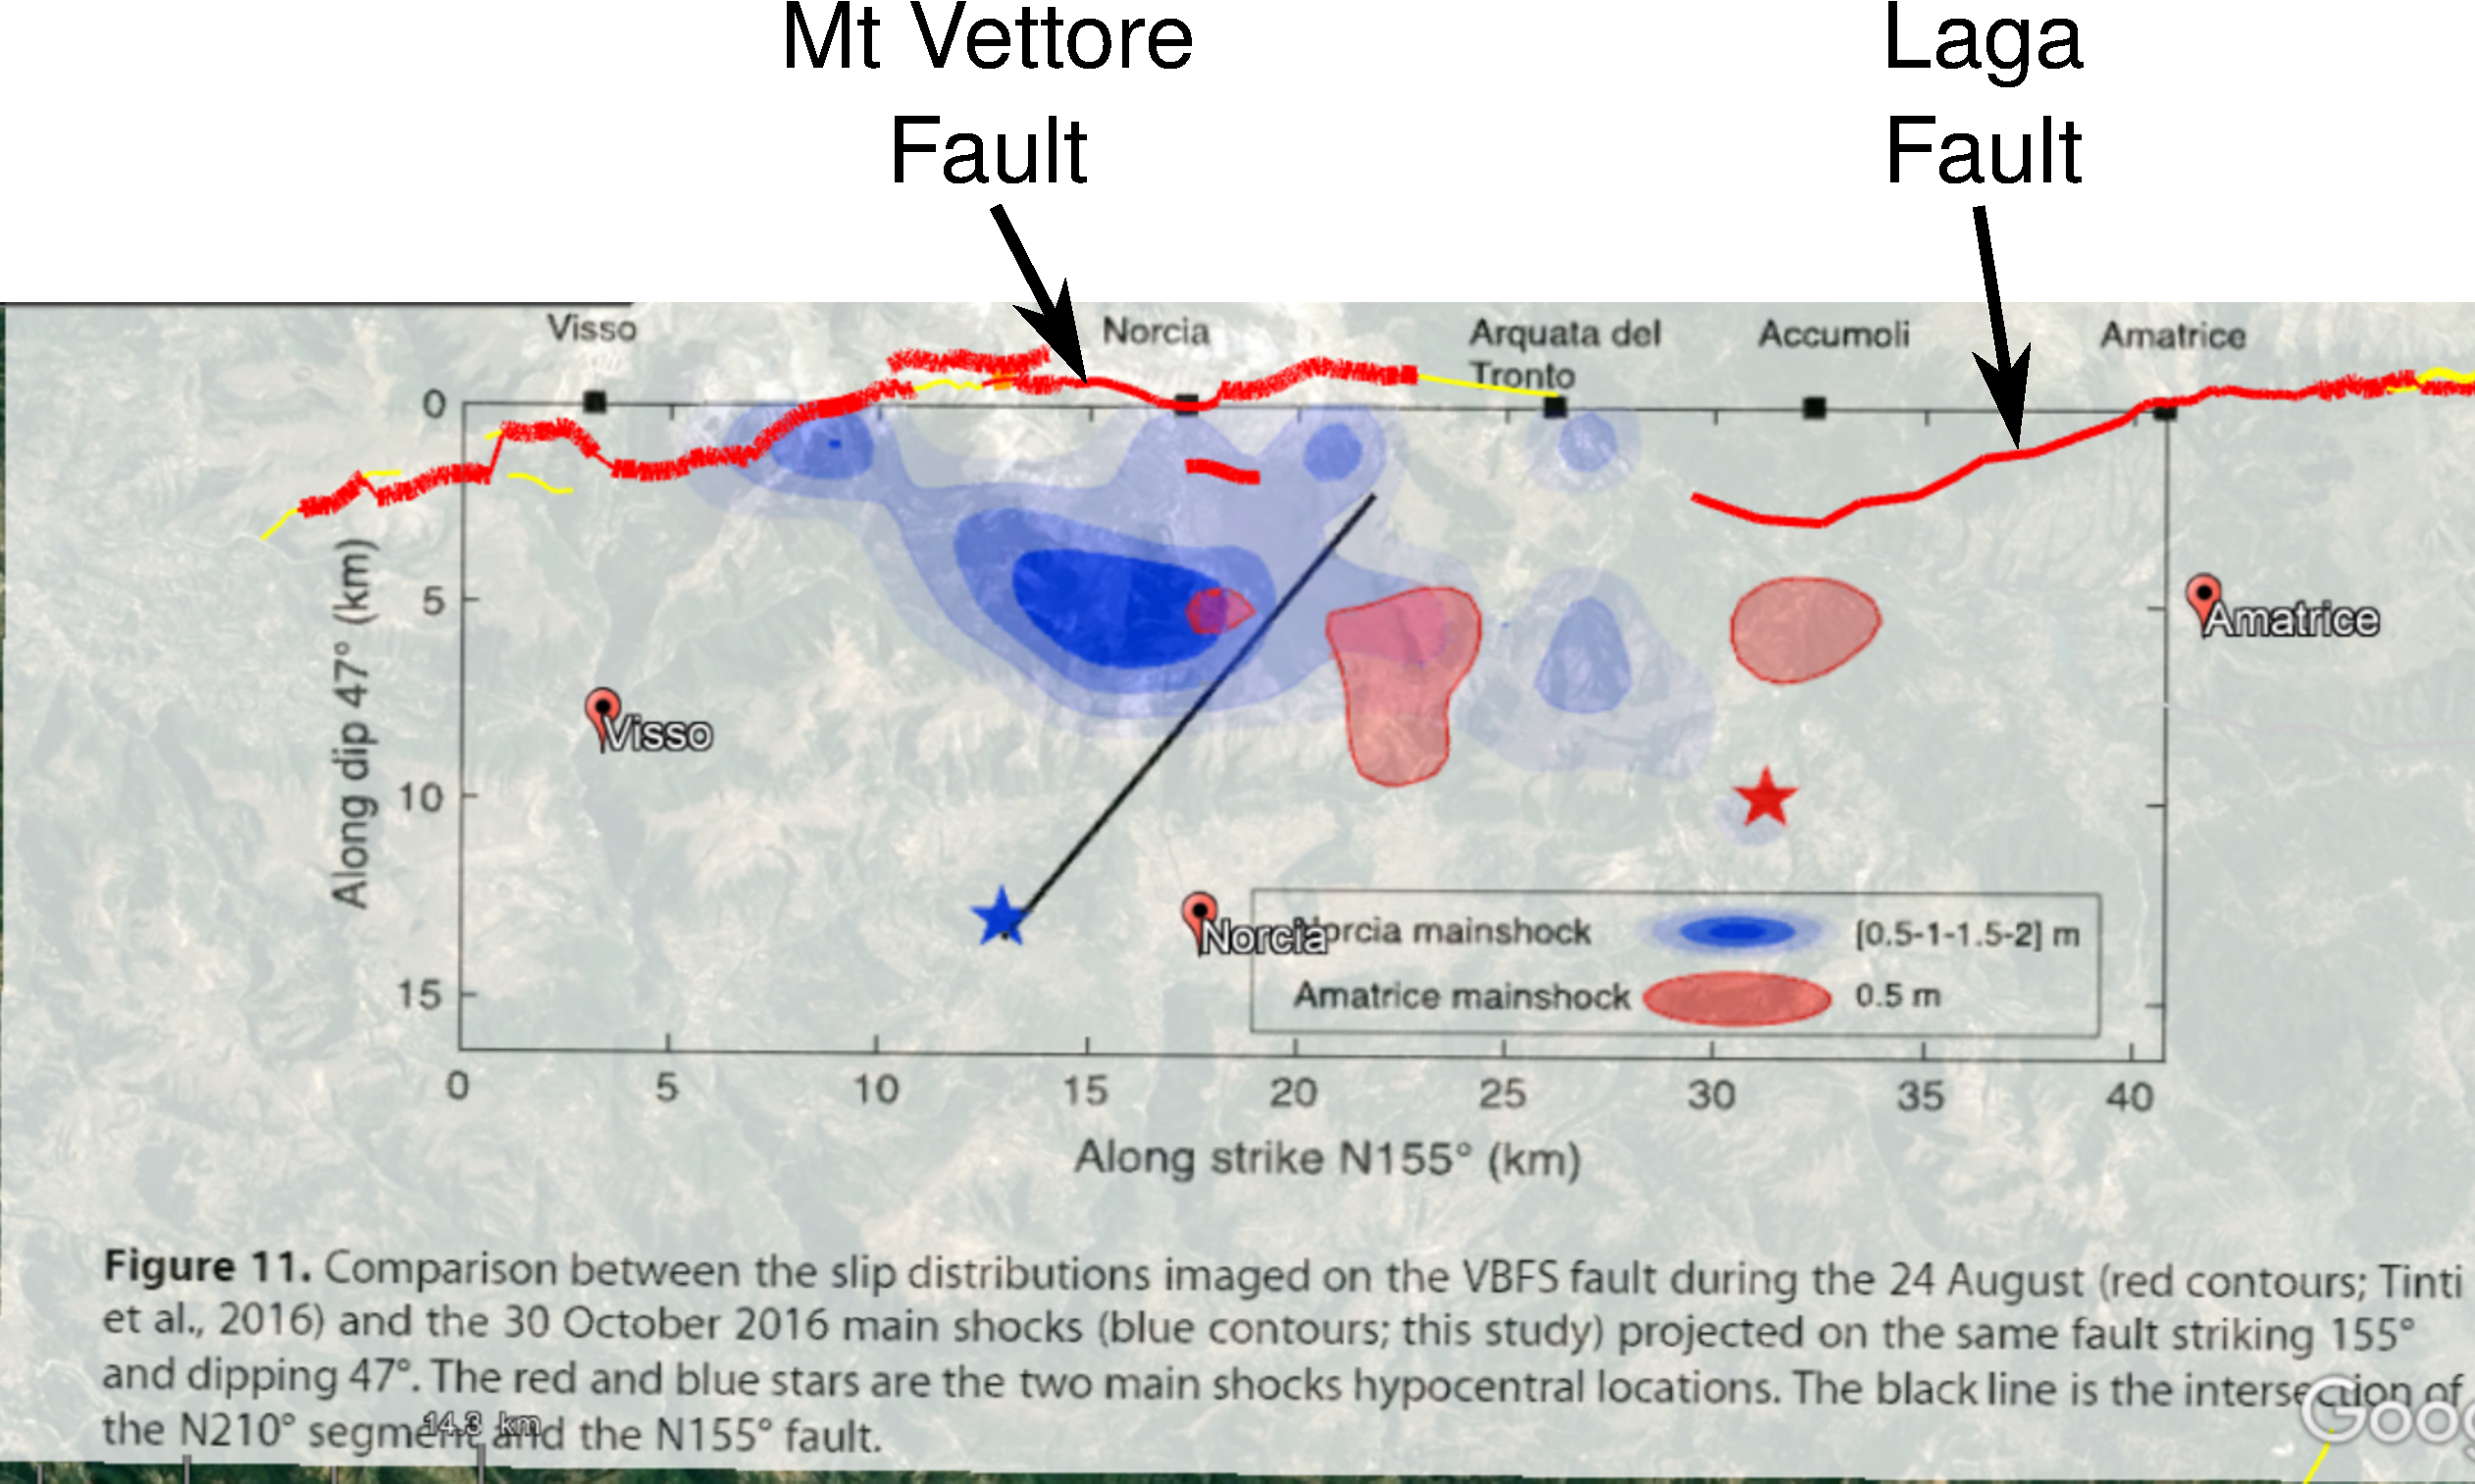
\includegraphics[width=1\linewidth]{images/amatrice_1.pdf}
 \end{minipage}
 \begin{minipage}{0.52\linewidth}
  {\bf Rupture jump across step-overs}
  \begin{itemize}
   \footnotesize \item \footnotesize Potential larger magnitudes?
   \vskip 0.3cm
   \item \footnotesize Conditions promoting this?
   \begin{itemize}
   \vskip 0.3cm
    \item \footnotesize Geometry
    \item \footnotesize Stress conditions
   \end{itemize}
   \vskip 0.3cm
   \item \footnotesize To enhance SHA!
  \end{itemize}
 \end{minipage}

 \begin{center}
 \vskip 0.3cm
   \underline{\bf \small Investigate the physical conditons}
   \underline{\bf \small promoting rupture jumps across step overs} 
   \underline{\bf \small regarding normal fault systems} 
  \vskip 0.3cm
  
 \end{center}
 {\scriptsize Previous studies focused on strike-slip fault systems: \cite{Galis_2015_ISS,Hu_2016_IEJ,Bai_2017_ESD,Li_2020_ERT,Oglesby_2008_RTJ}, and more ... } 
 \addtocounter{framenumber}{-1}
 
\end{frame}




\section{Preliminary exploration}

\begin{frame}
 {Preliminary exploration: Geometry and settings}
 
  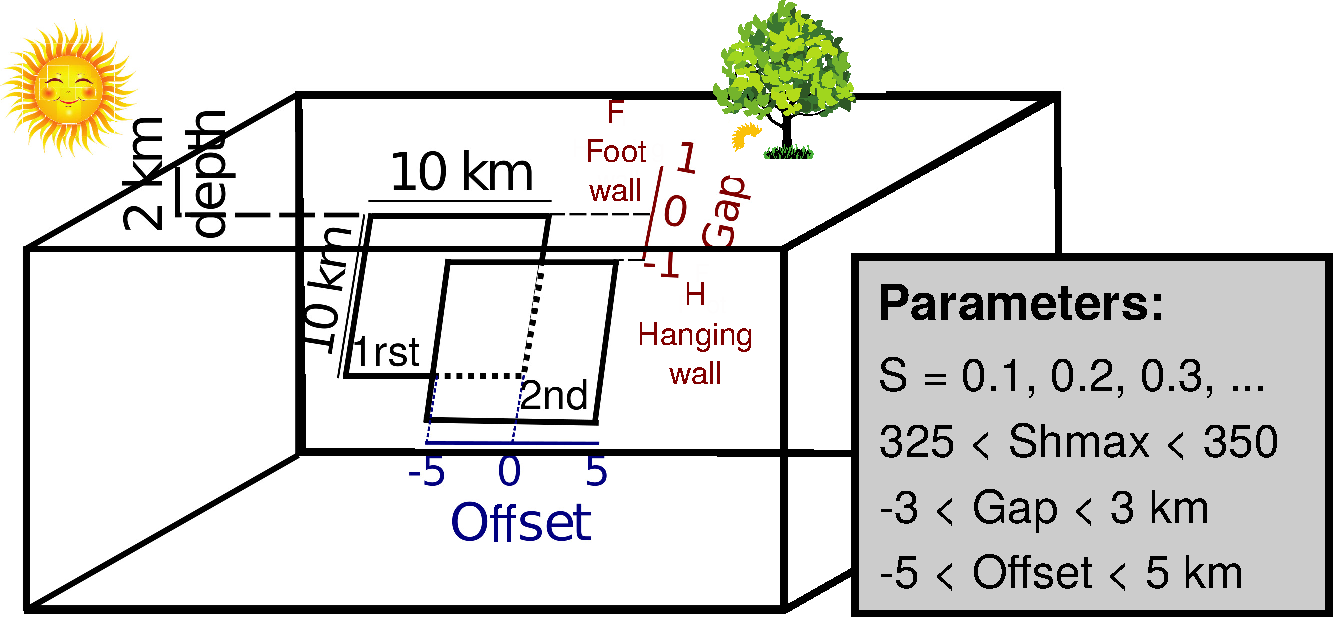
\includegraphics[width=1\linewidth]{images/schematic_view_param_new}
 
 \hfill {\small \citep[www.seissol.org; e.g.,][]{Wollherr_2018_OFP, Ulrich_2019_CPB}}
 
\end{frame}


\begin{frame}
 
 \centering \huge SMALL PUBLICIT\'E !!
 \\ \ \\
% \\
 SimModeler: meshing engine
 \\
 \&
 \\ 
% \\
 SeisSol: dynamic rupture modeling
 
 
\end{frame}



\begin{frame}
 {SimModeler software : Modeling complex fault geometry}
 
 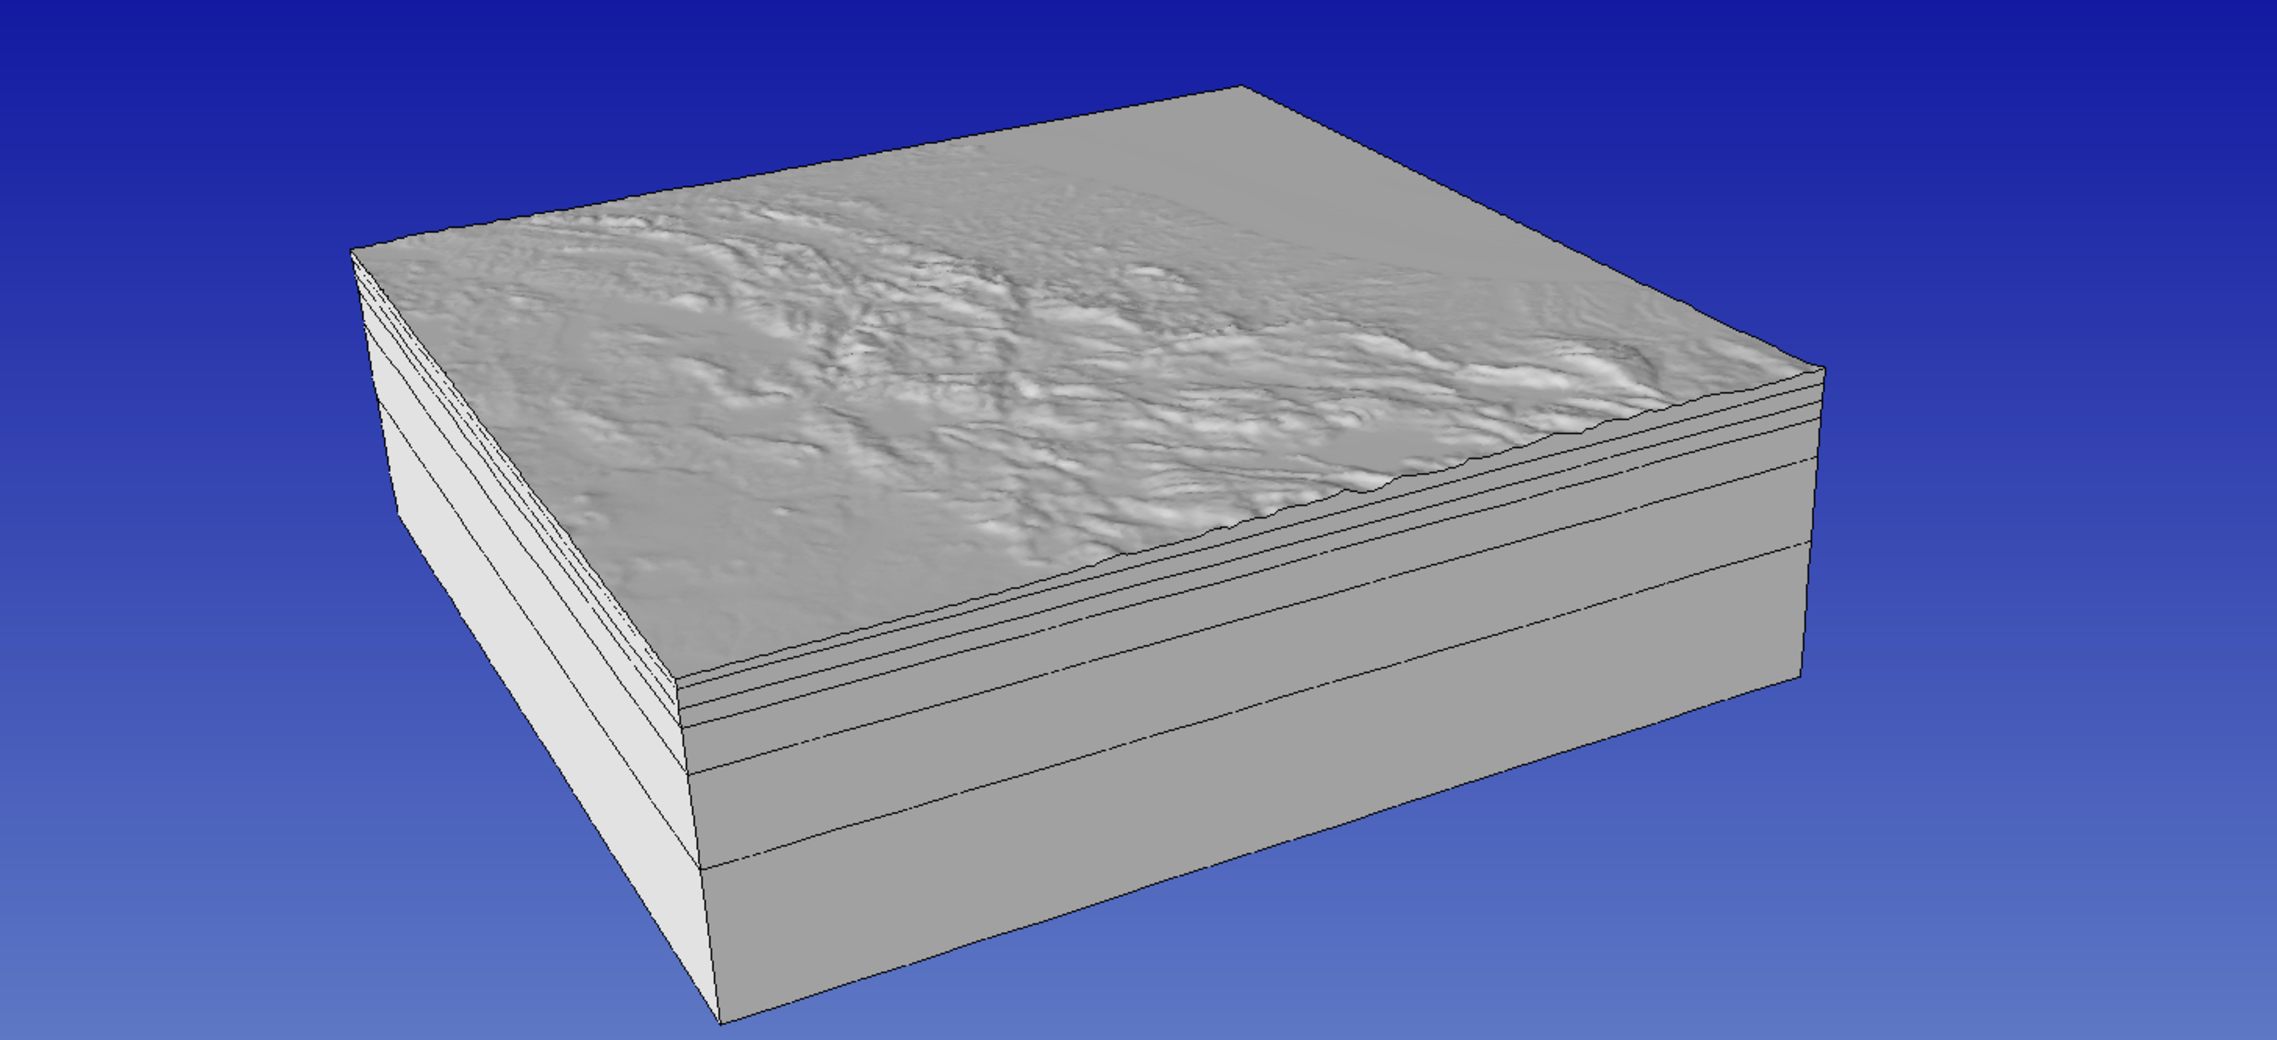
\includegraphics[width=1\linewidth]{images/simmodeler1}
 
\end{frame}

\begin{frame}
 {SimModeler software : Modeling complex fault geometry}
 
 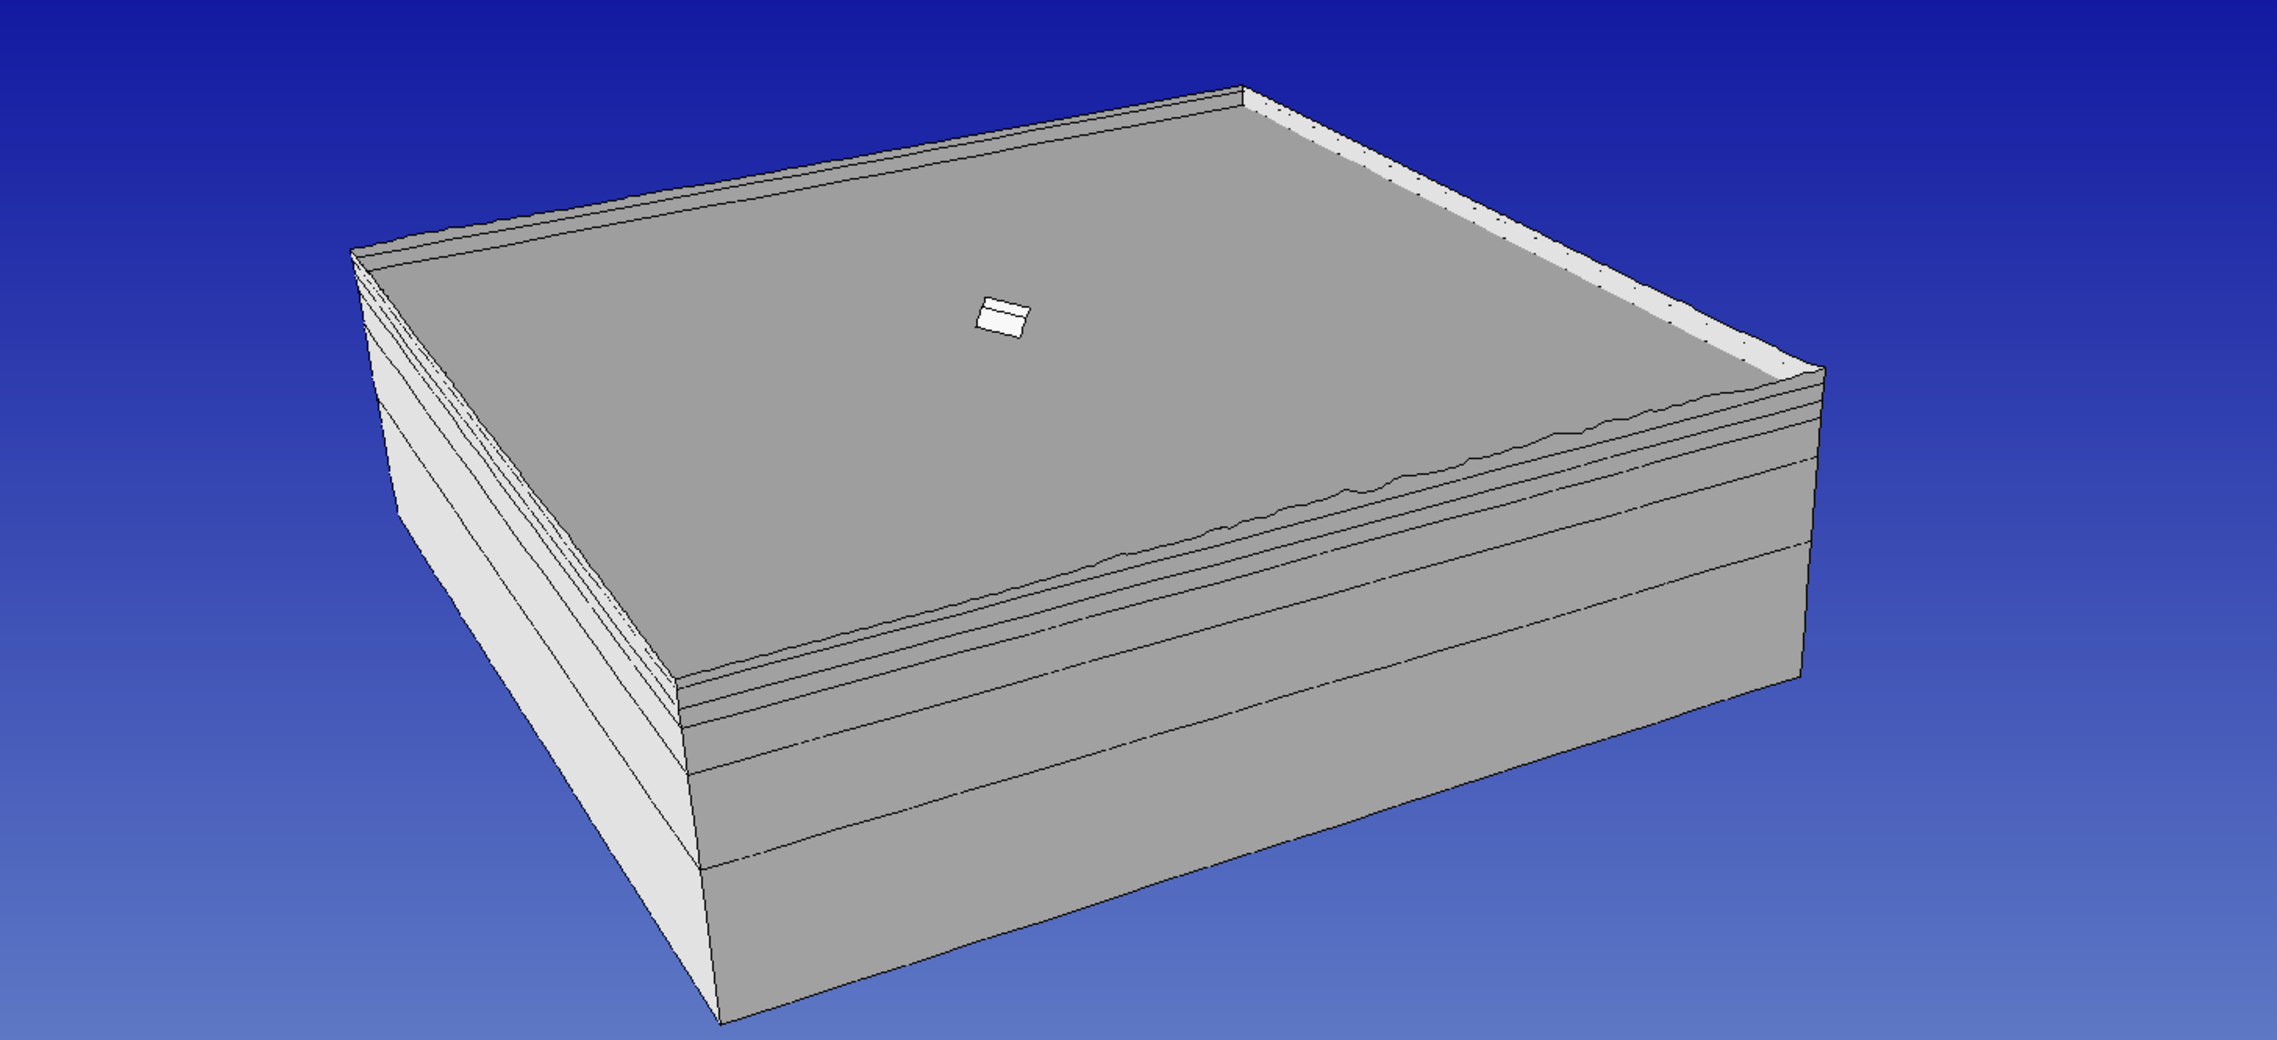
\includegraphics[width=1\linewidth]{images/simmodeler2}
 
\end{frame}

\begin{frame}
 {SimModeler software : Modeling complex fault geometry}
 
 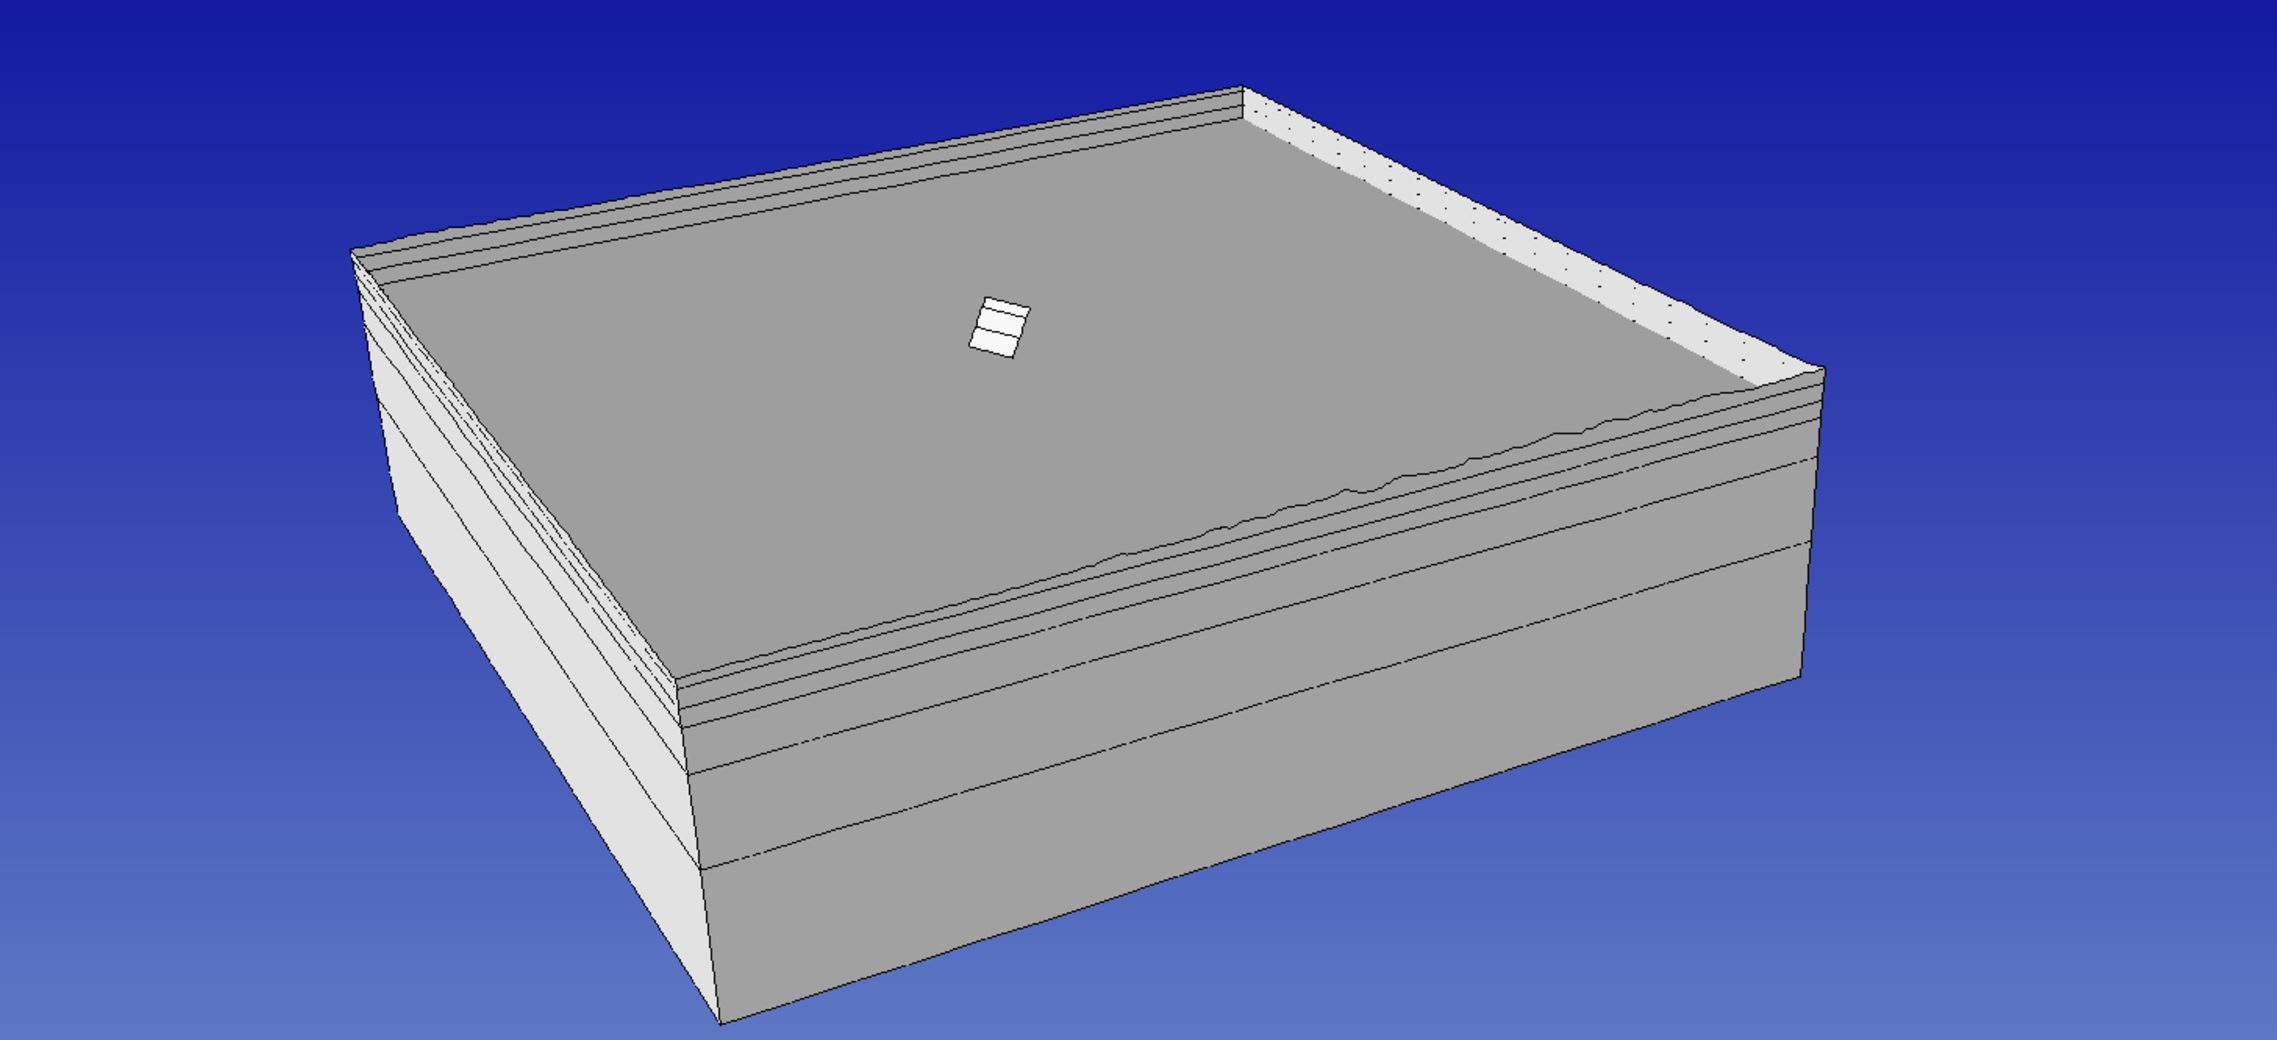
\includegraphics[width=1\linewidth]{images/simmodeler3}
 
\end{frame}

\begin{frame}
 {SimModeler software : Modeling complex fault geometry}
 
 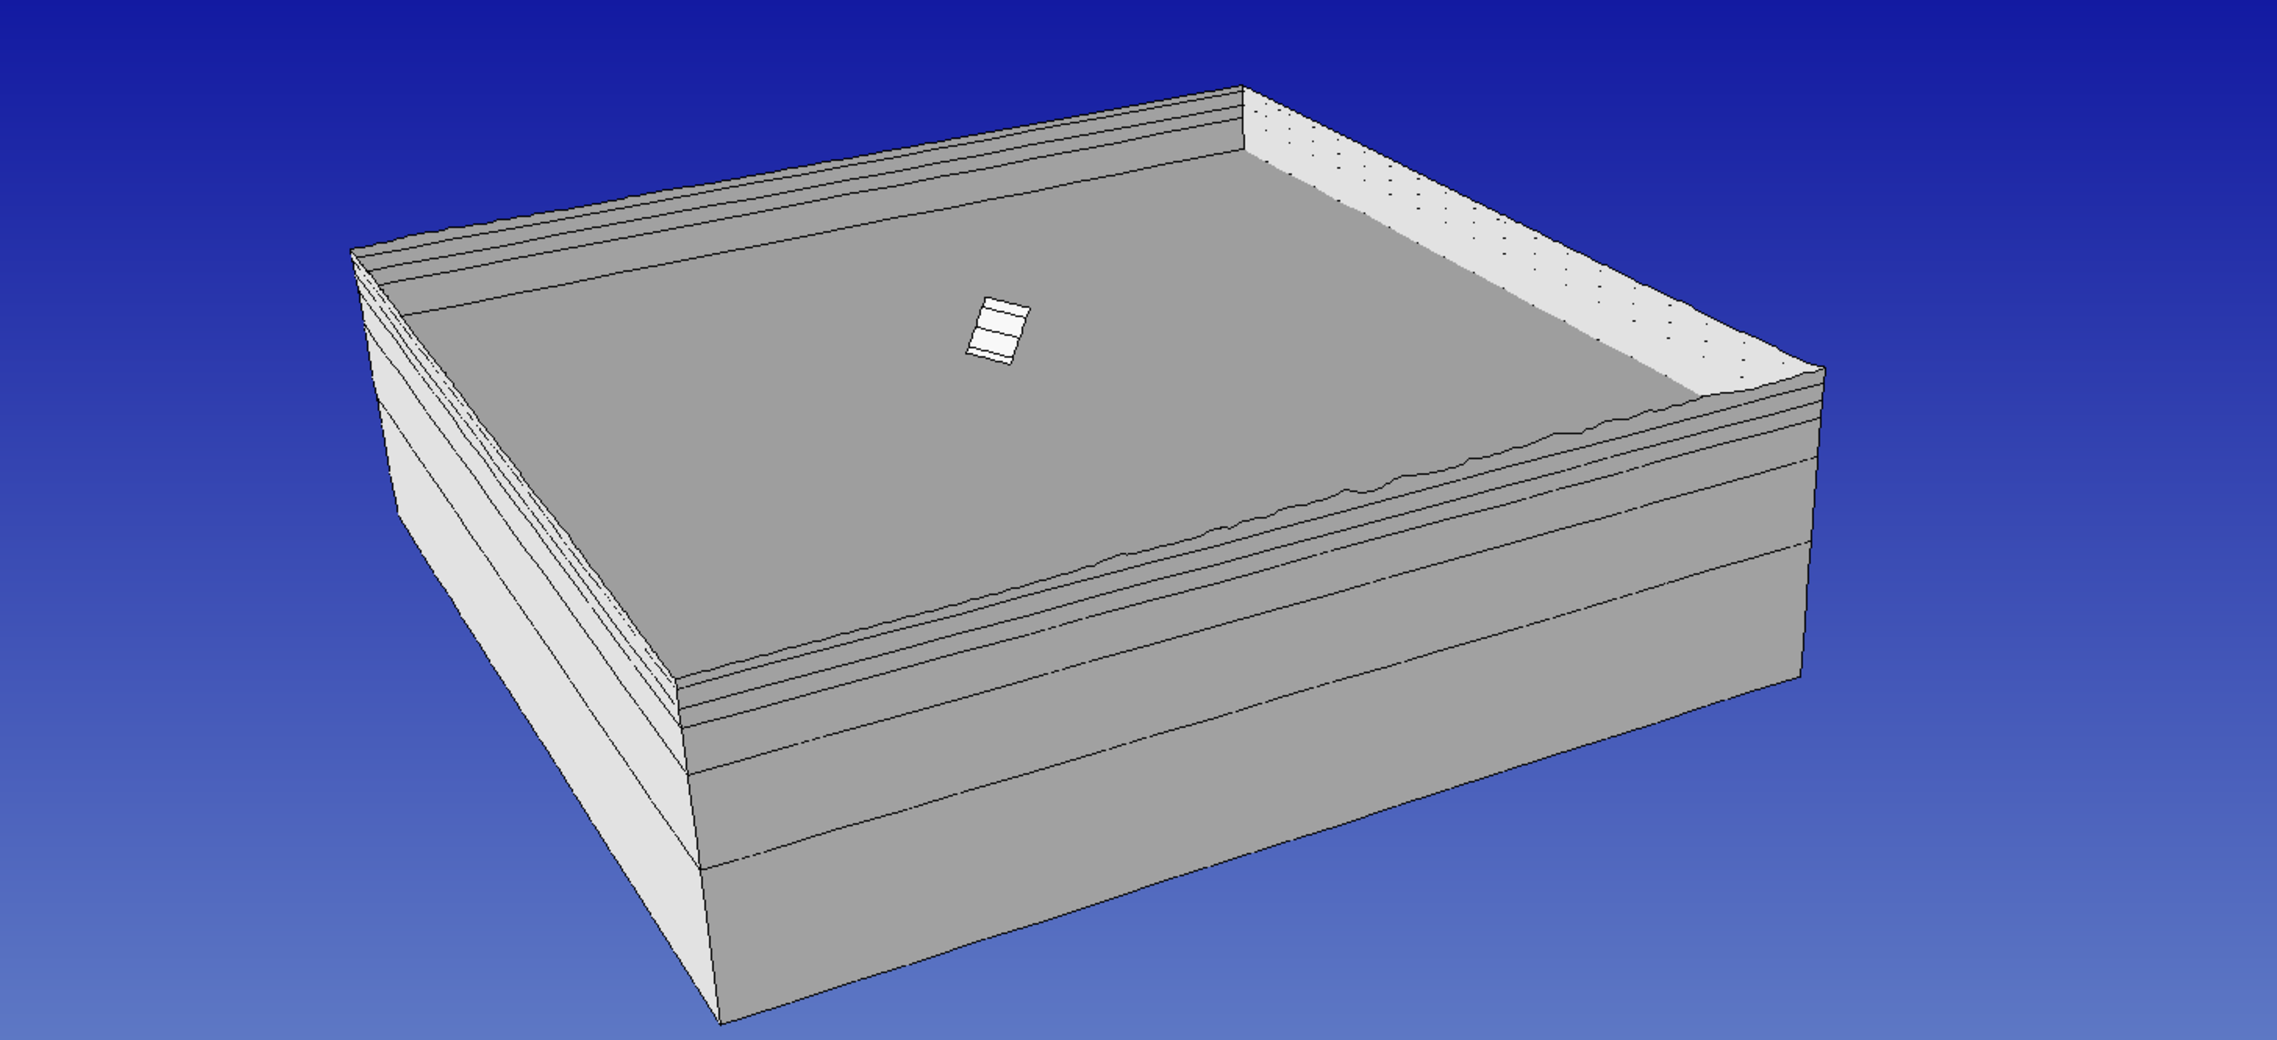
\includegraphics[width=1\linewidth]{images/simmodeler4}
 
\end{frame}

\begin{frame}
 {SimModeler software : Modeling complex fault geometry}
 
 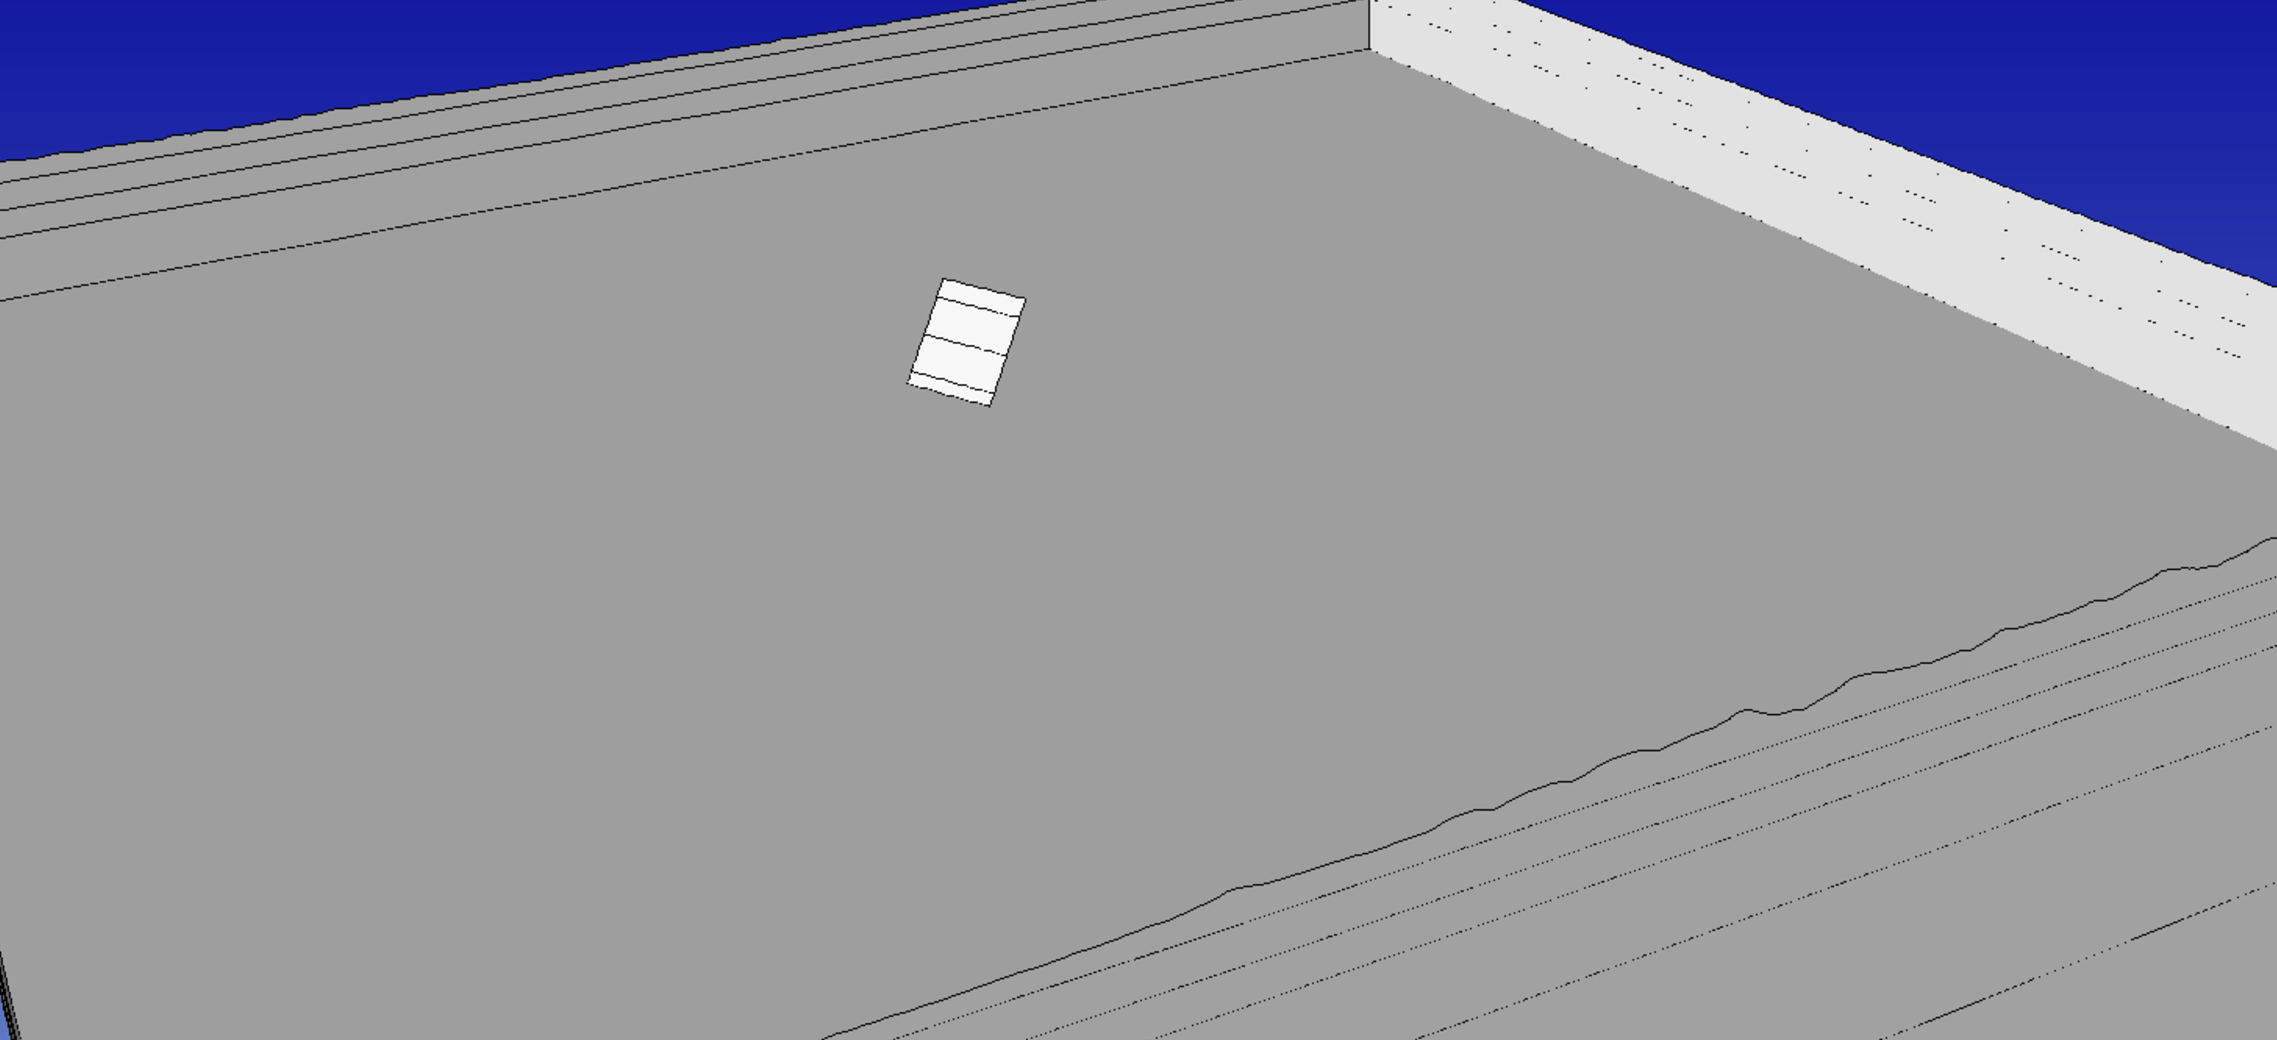
\includegraphics[width=1\linewidth]{images/simmodeler5}
 
\end{frame}

\begin{frame}
 {SimModeler software : Modeling complex fault geometry}
 
 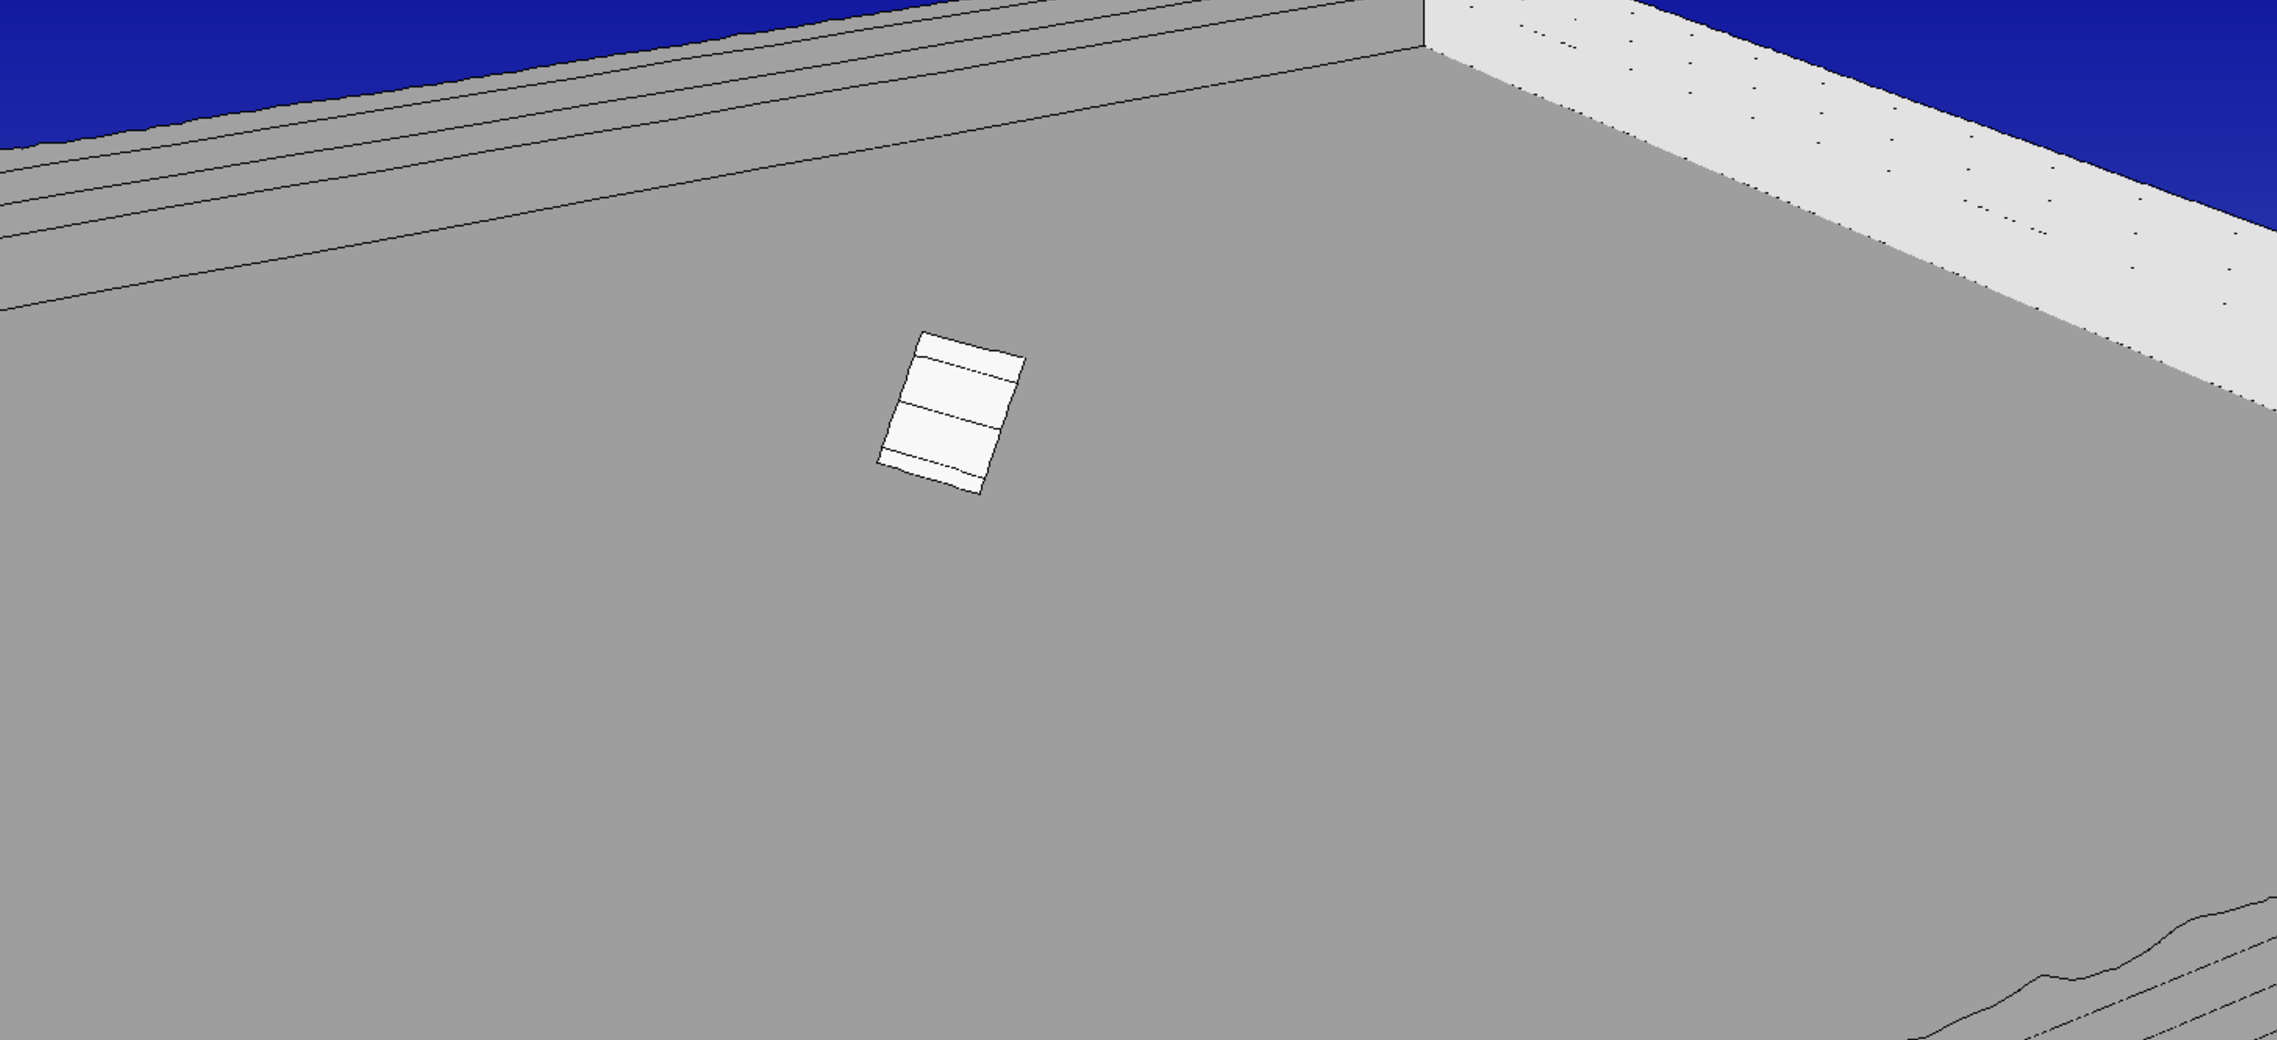
\includegraphics[width=1\linewidth]{images/simmodeler6}
 
\end{frame}

\begin{frame}
 {SimModeler software : Modeling complex fault geometry}
 
 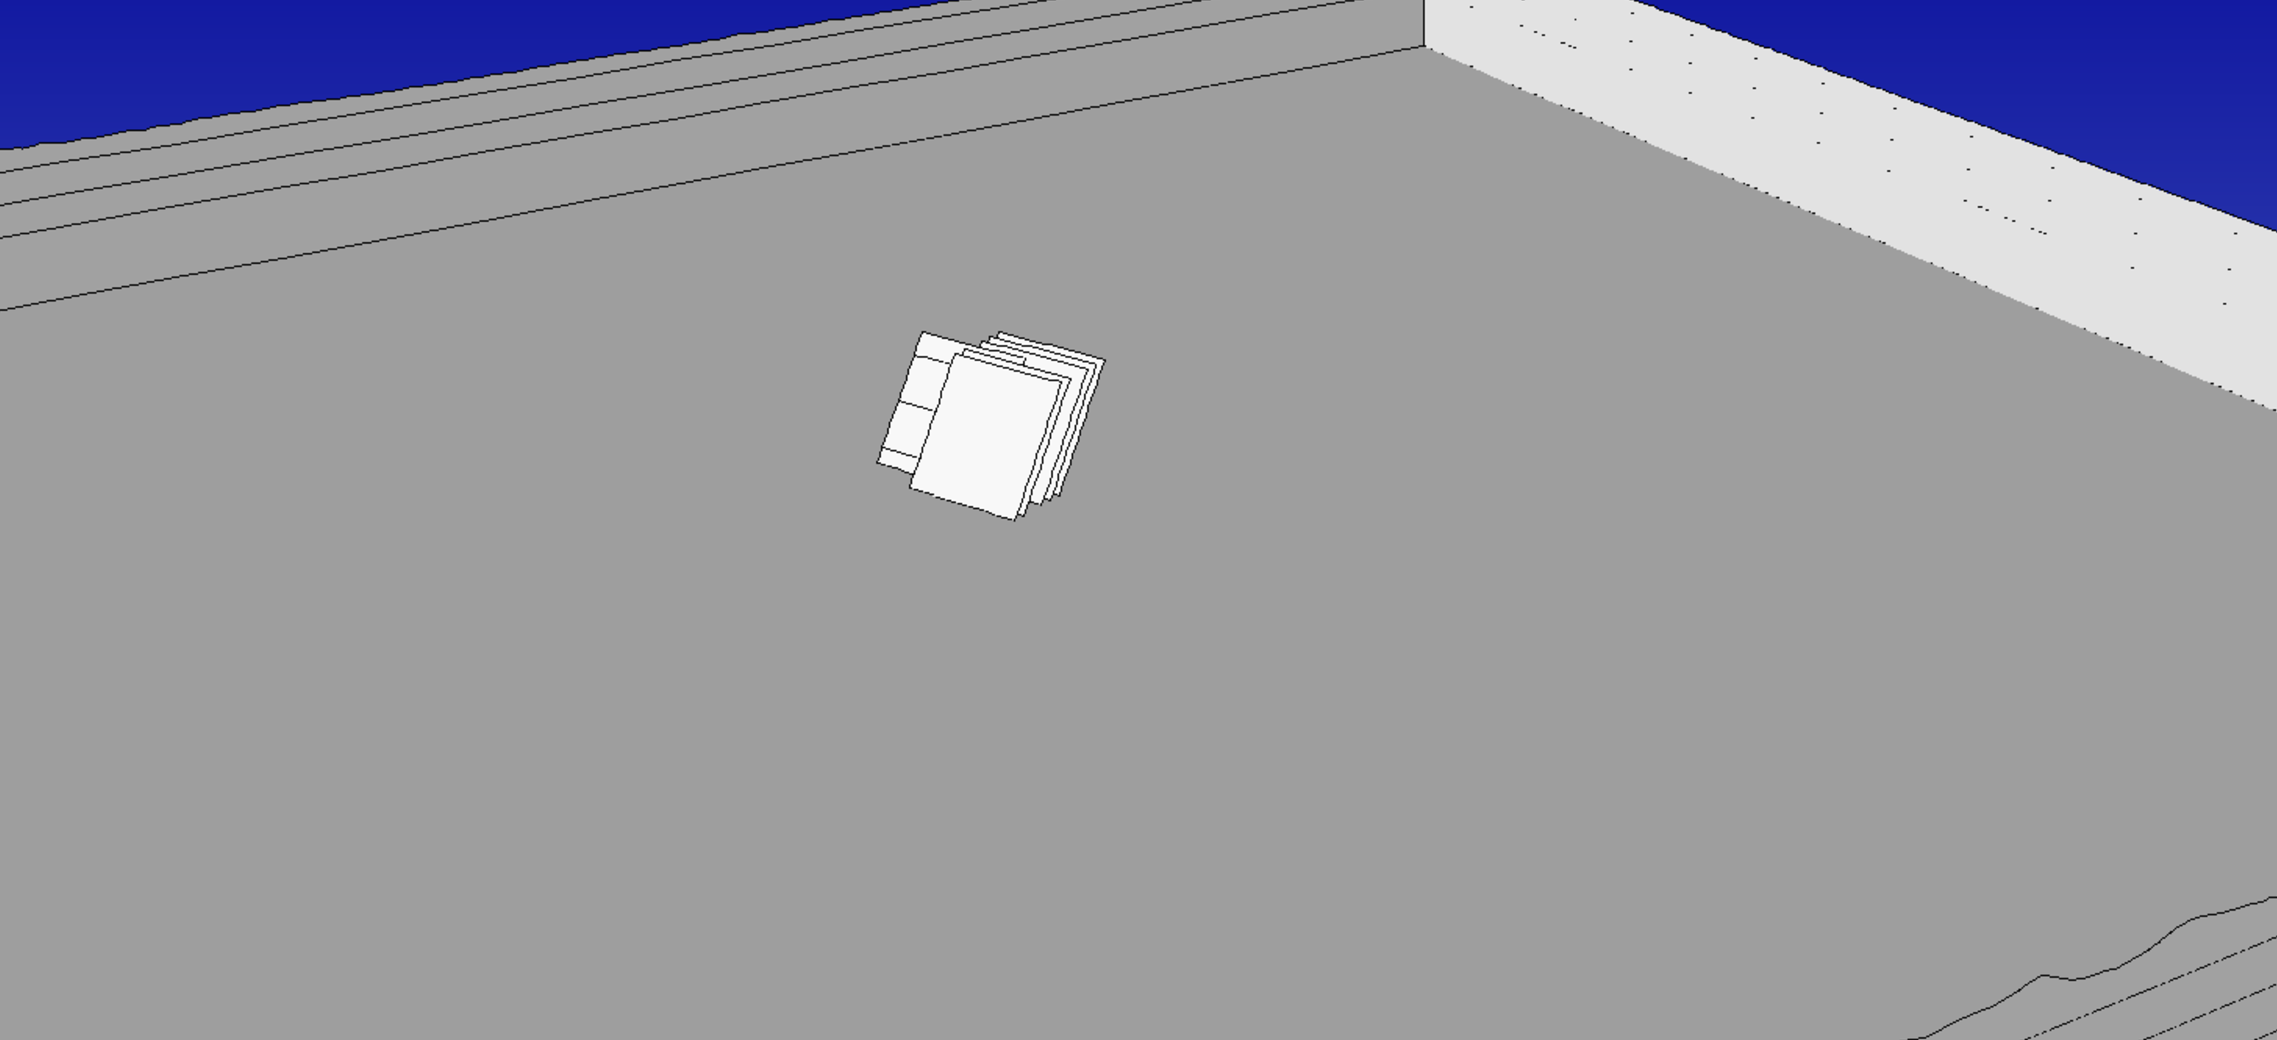
\includegraphics[width=1\linewidth]{images/simmodeler7}
 
\end{frame}

\begin{frame}
 {SimModeler software : Modeling complex fault geometry}
 
 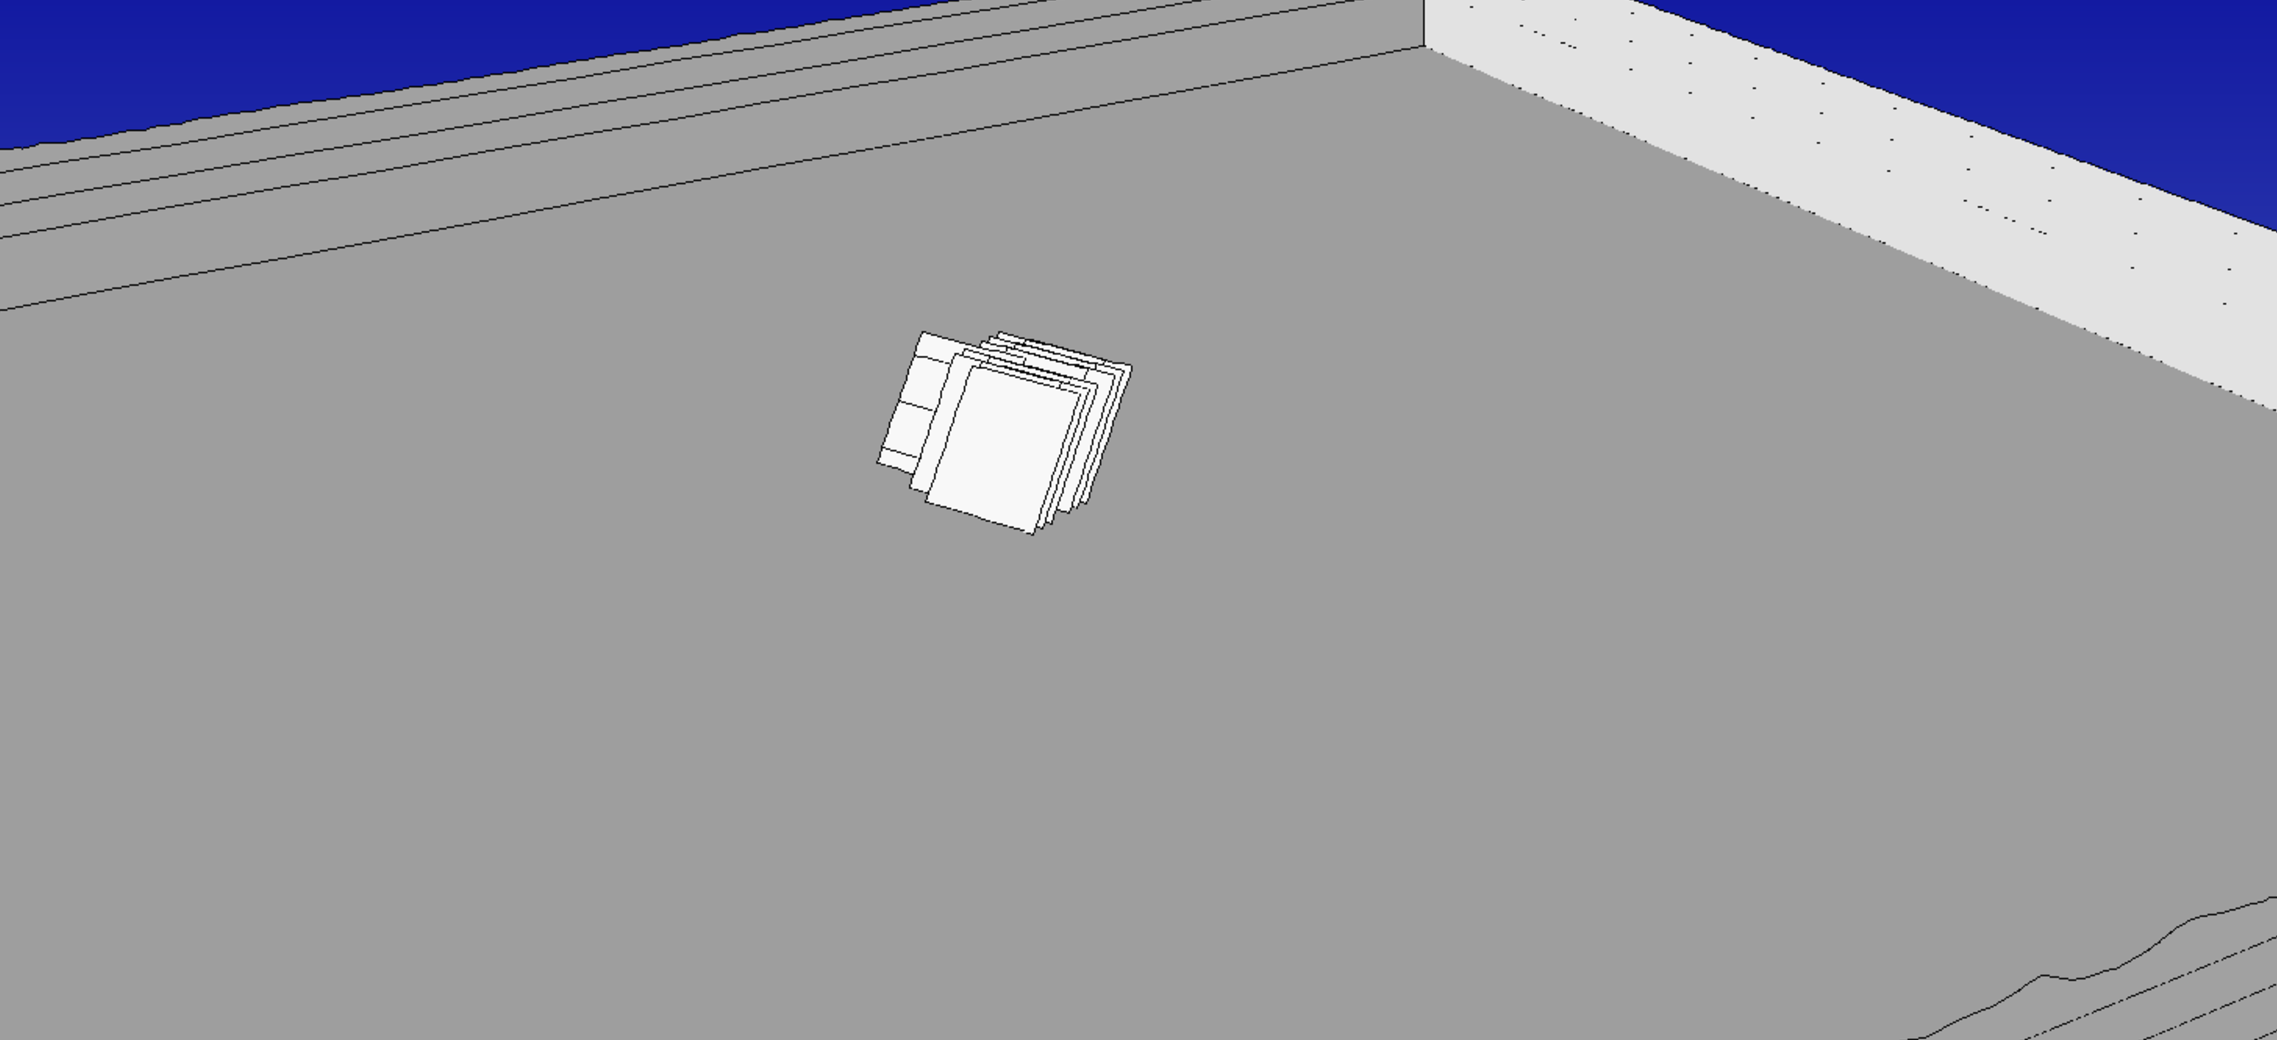
\includegraphics[width=1\linewidth]{images/simmodeler8}
 
\end{frame}

\begin{frame}
 {SimModeler software : Modeling complex fault geometry}
 
 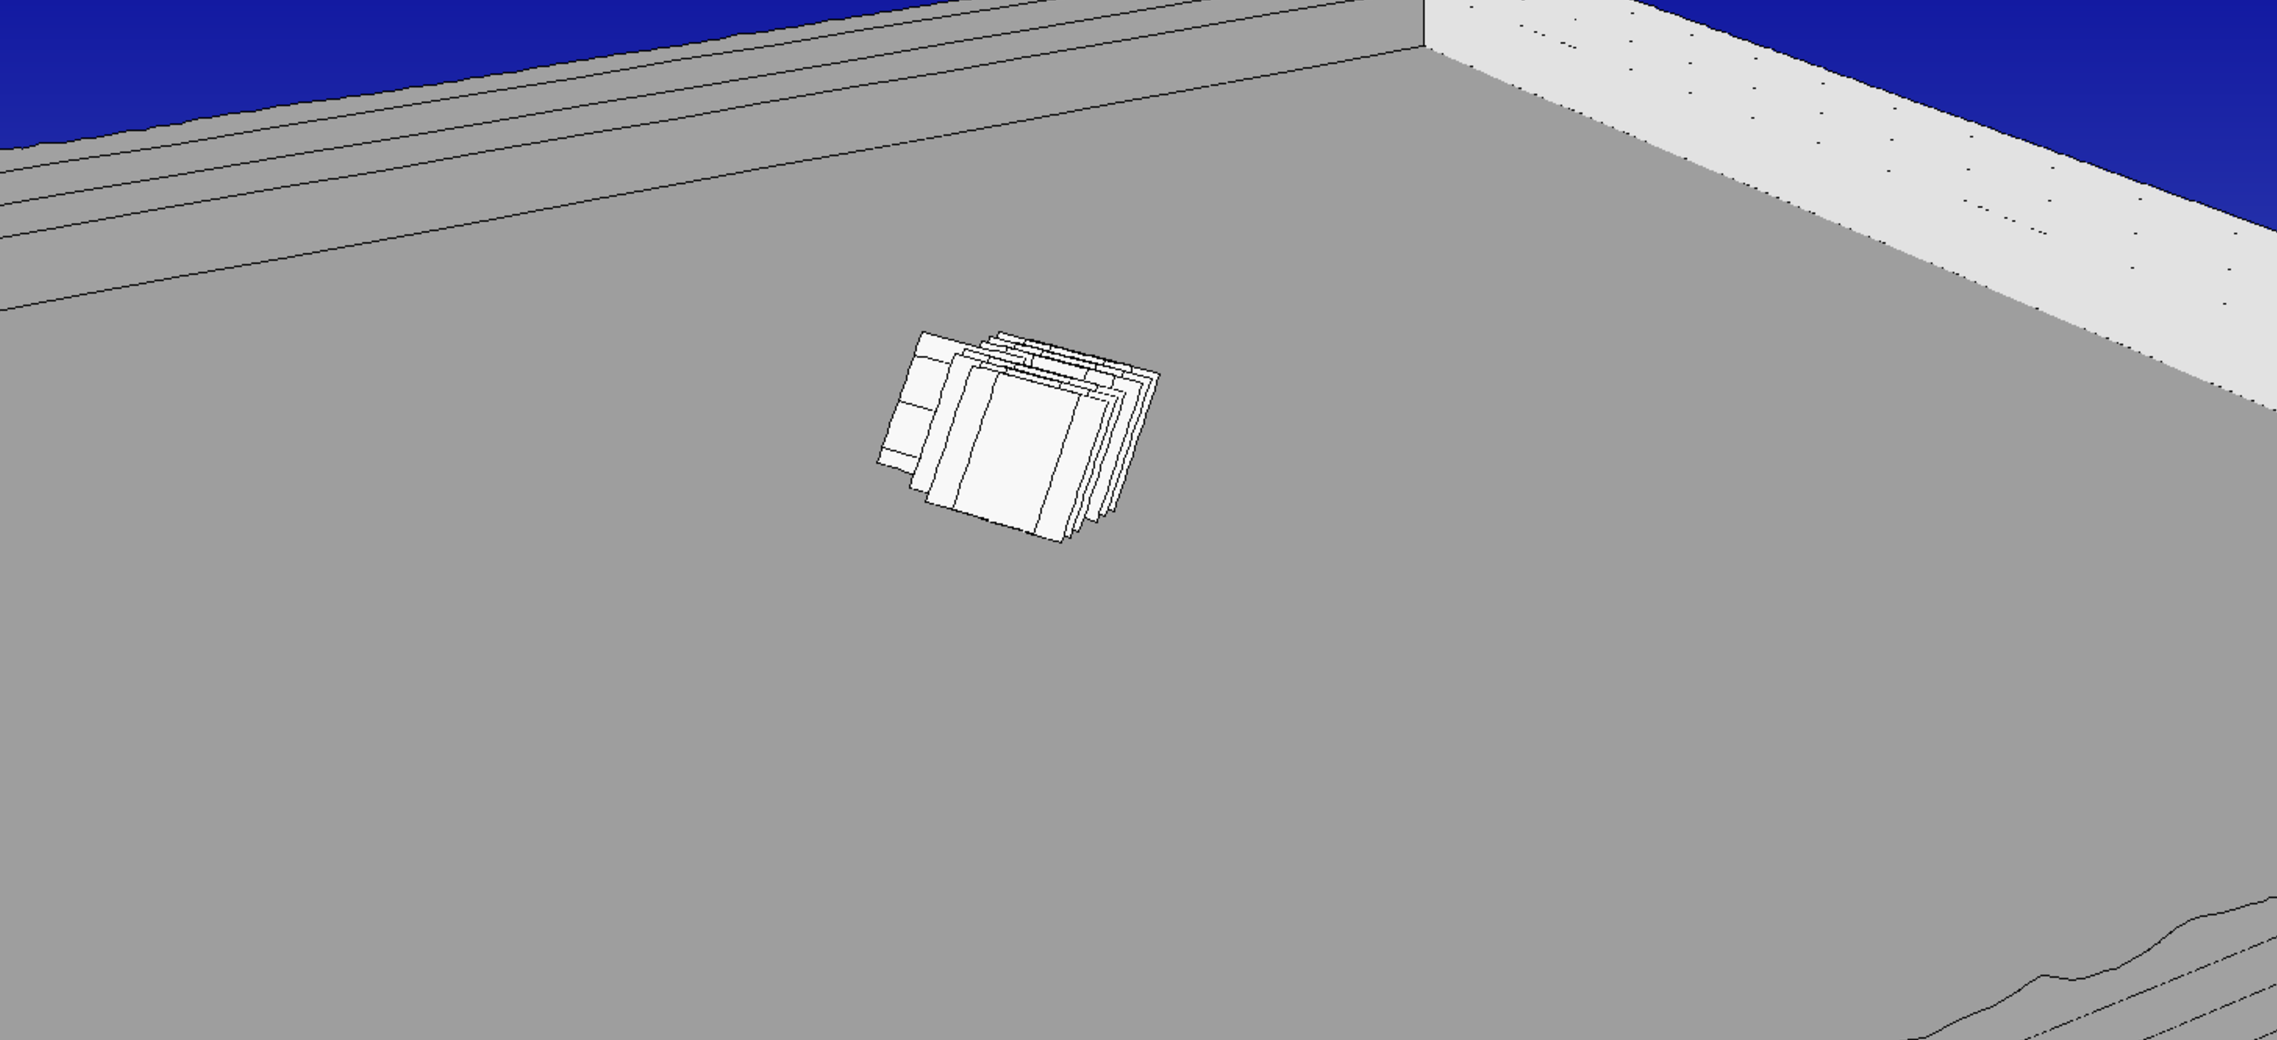
\includegraphics[width=1\linewidth]{images/simmodeler9}
 
\end{frame}

\begin{frame}
 {SimModeler software : Modeling complex fault geometry}
 
 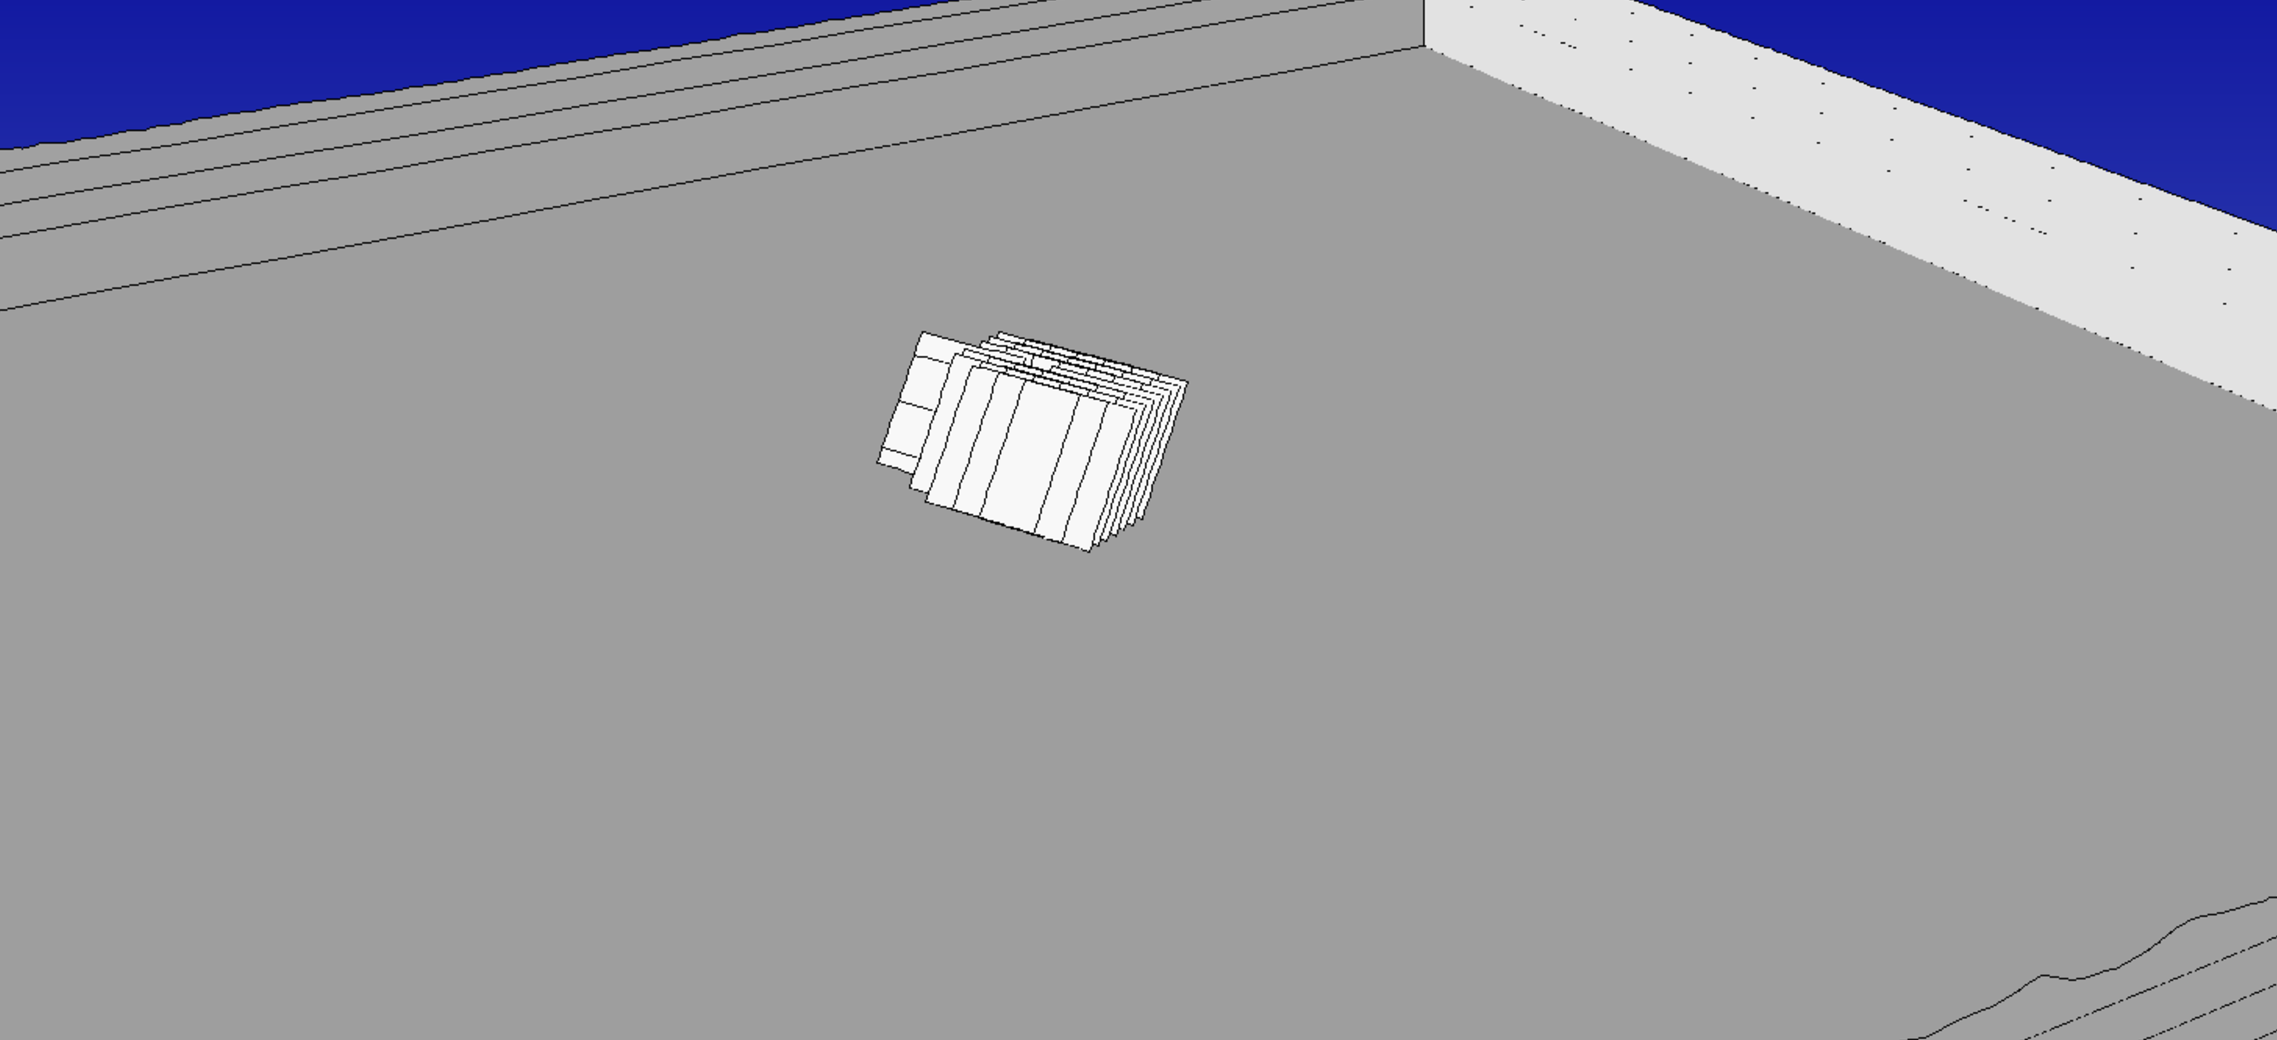
\includegraphics[width=1\linewidth]{images/simmodeler10}
 
\end{frame}

\begin{frame}
 {SimModeler software : Modeling complex fault geometry}
 
 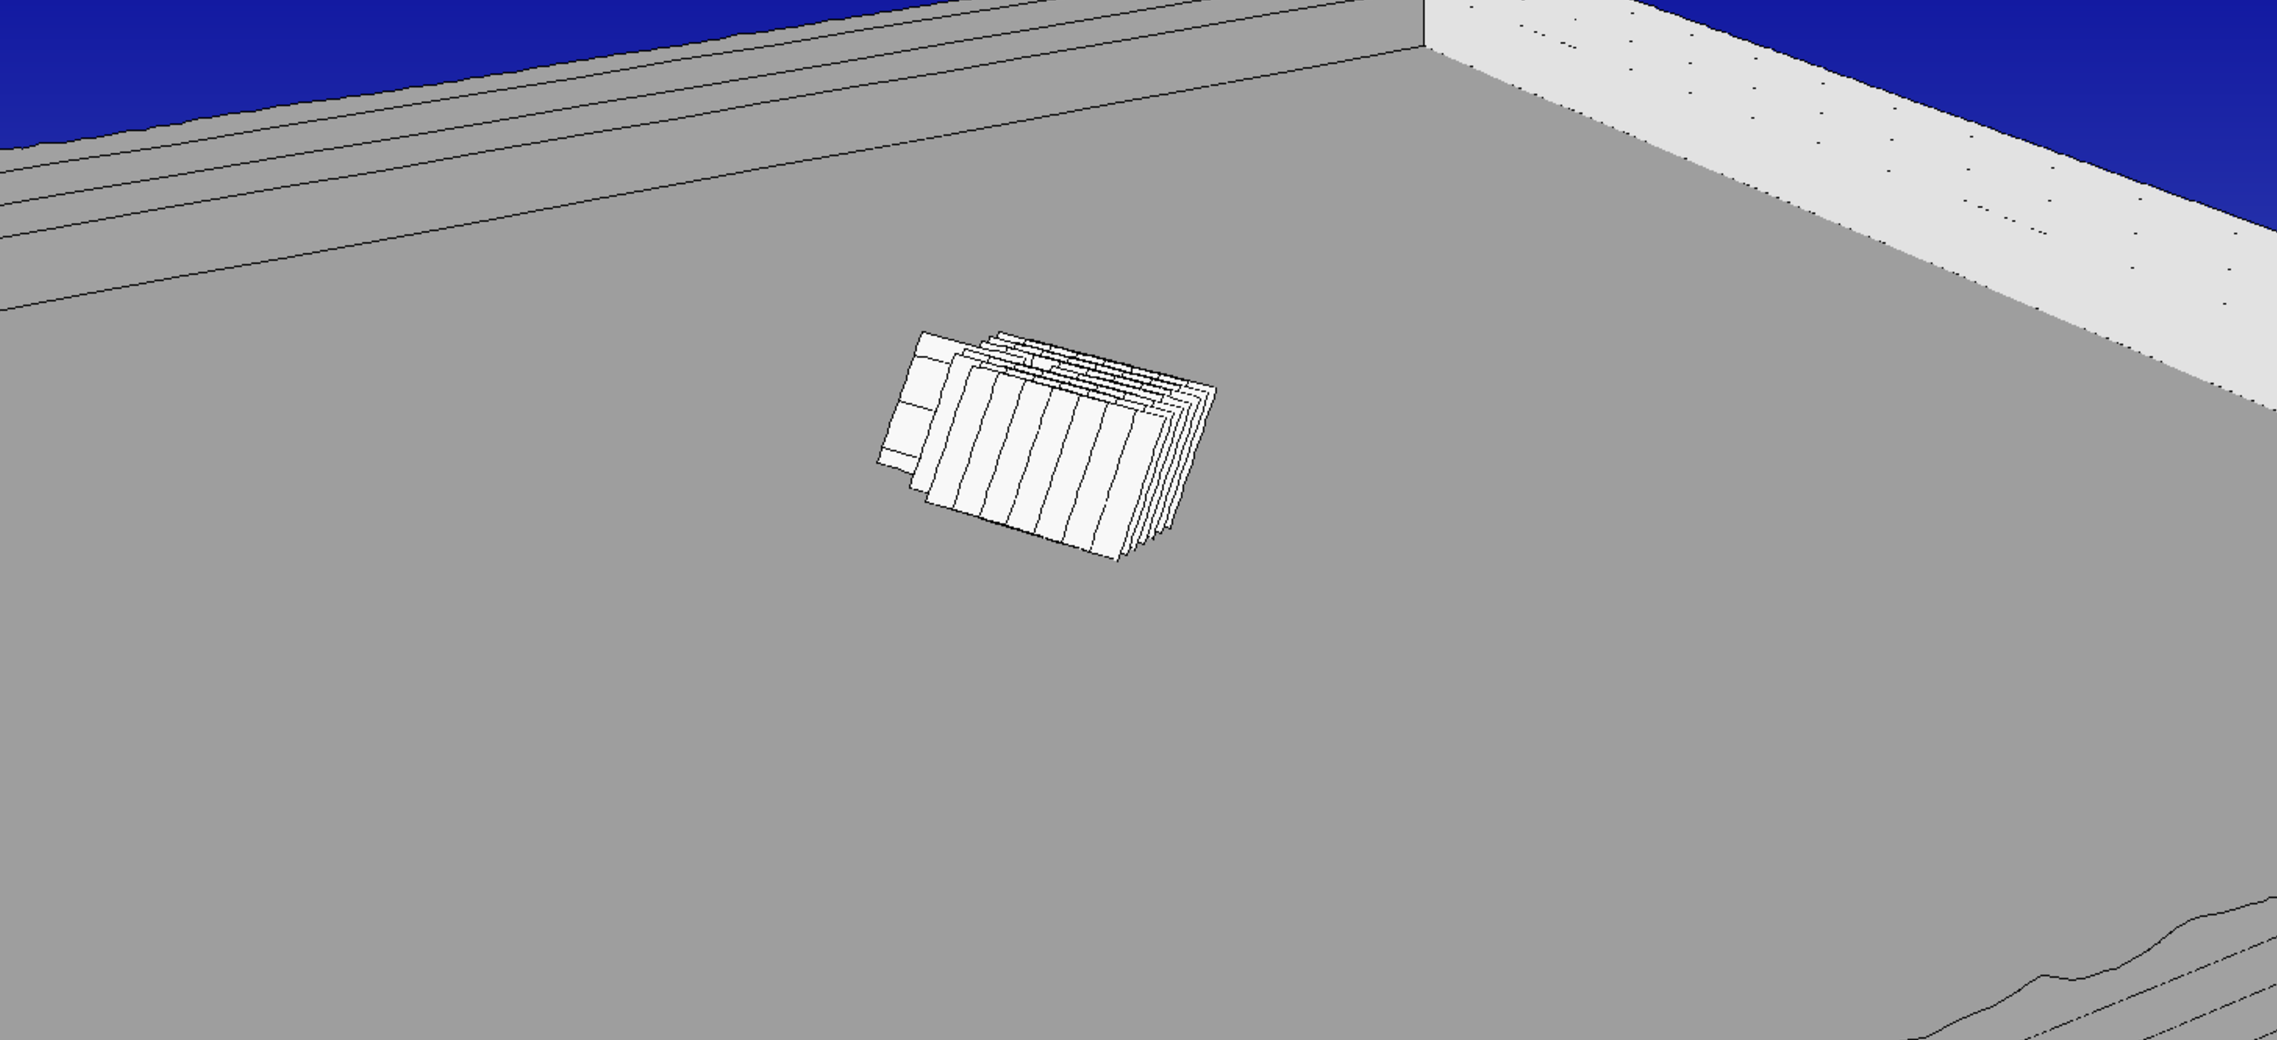
\includegraphics[width=1\linewidth]{images/simmodeler11}
 
\end{frame}

\begin{frame}
 {SimModeler software : Modeling complex fault geometry}
 
 \begin{minipage}{0.4\linewidth}
 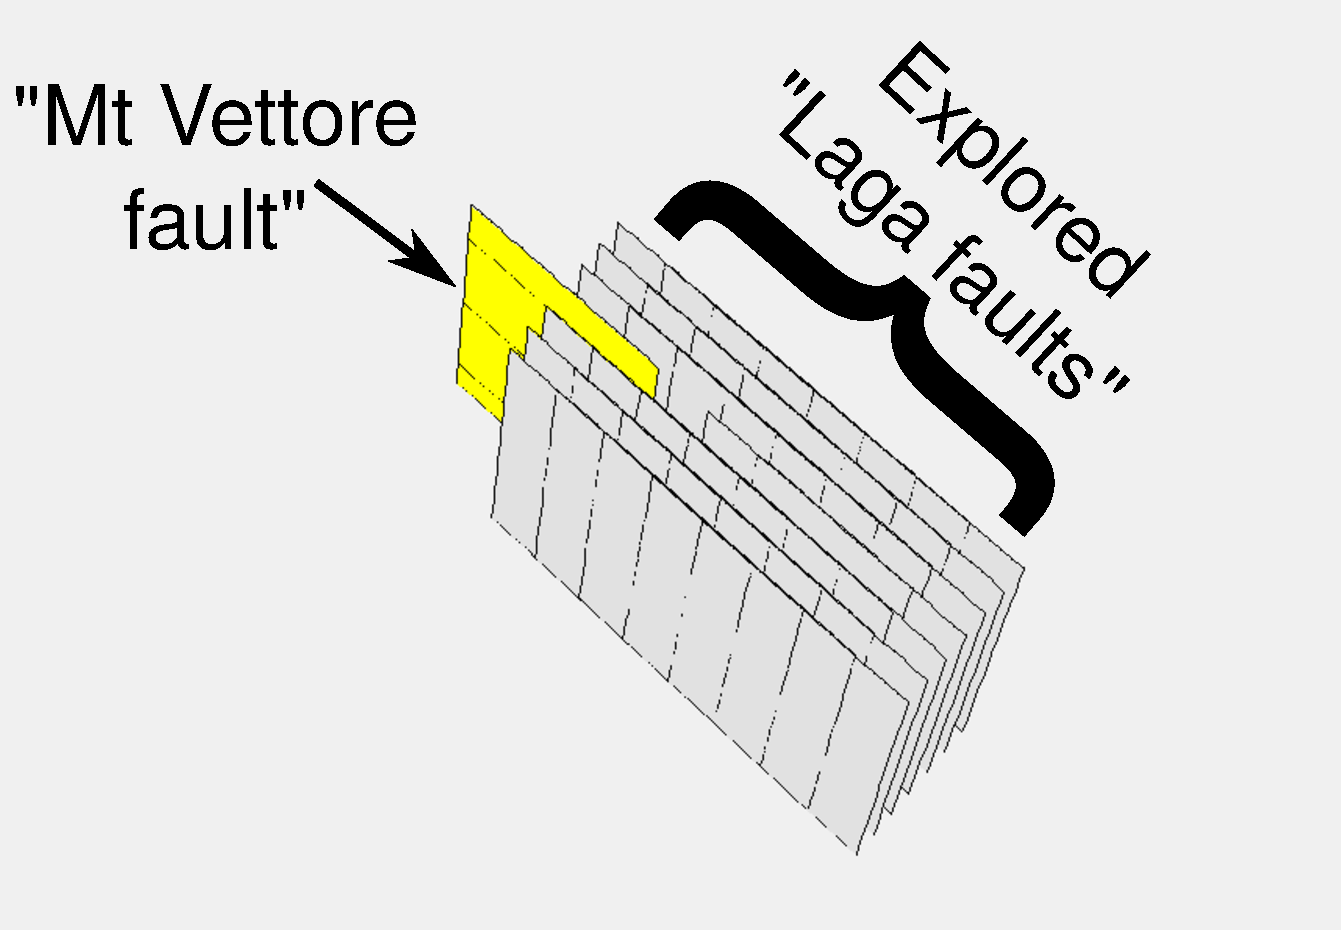
\includegraphics[width=1\linewidth]{images/simmodeler12.pdf} \\  
 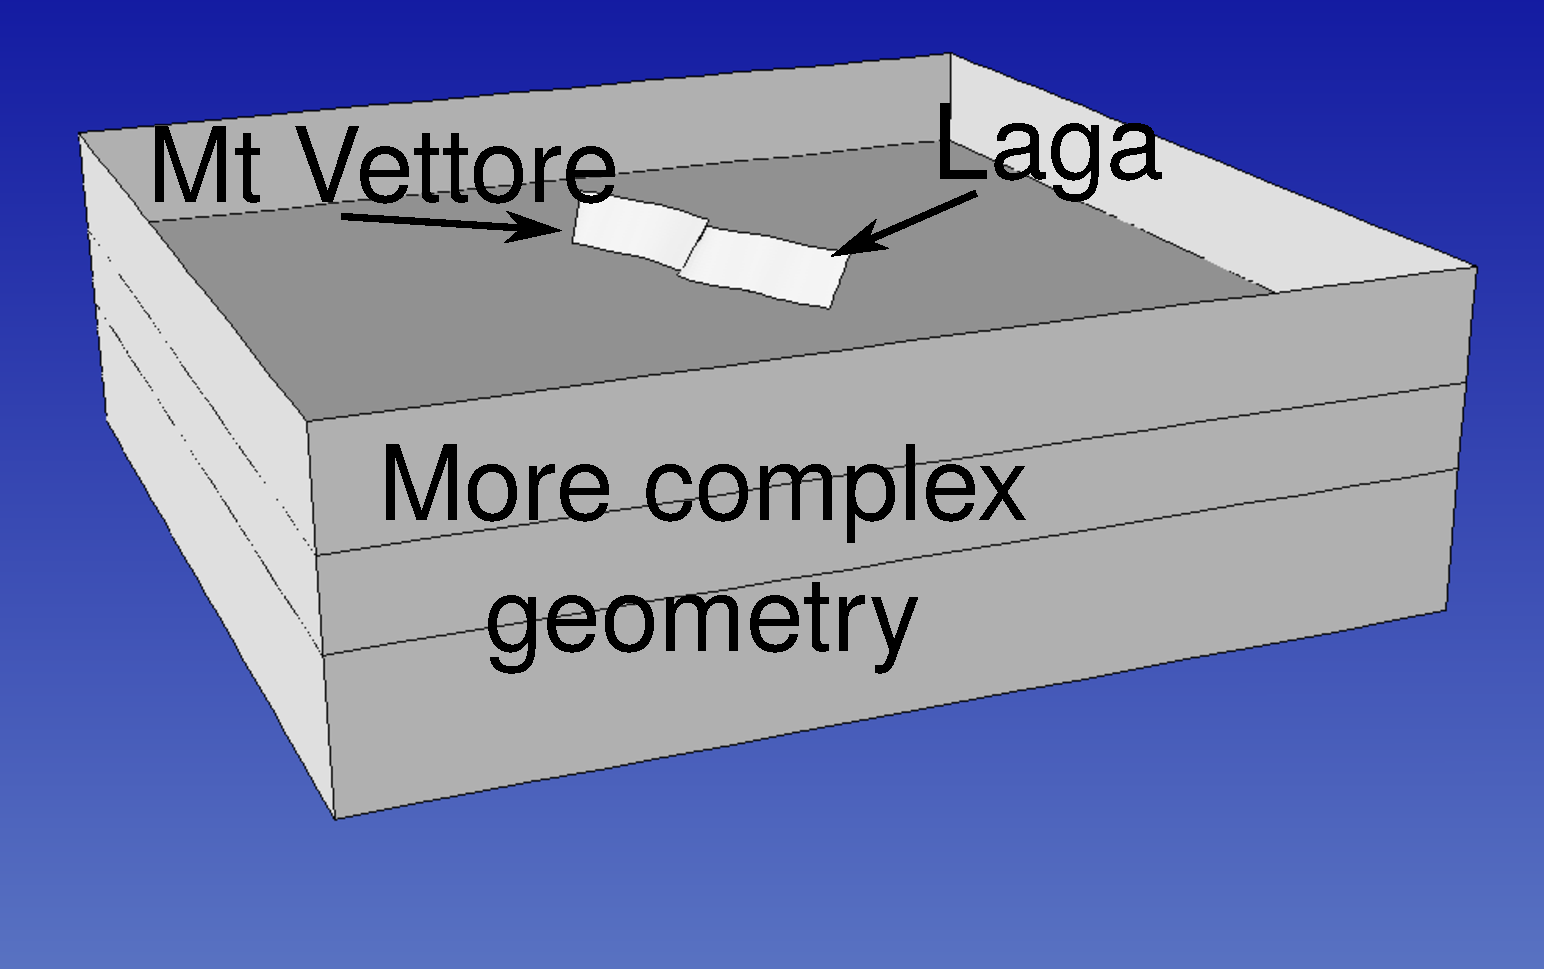
\includegraphics[width=1\linewidth]{images/simmodeler13.pdf}  
 \end{minipage}
 \begin{minipage}{0.58\linewidth}
 {\bf SimModeler \& SimModSuite}
 \vskip 0.5cm
  \begin{itemize}
   \item Complex mesh \& fault geometries \pause
   \item Mesh adaptivity \pause
   \item Simple user-friendly interface \pause
   \item Academic {\bf Free} License \pause
   \item Available documentation \pause
   \item Currently being installed on IST-OAR ... Thanks Jean-Noel!
  \end{itemize}
 \end{minipage}

 
\end{frame}


\begin{frame}
 
 
 \huge \center SeisSol dynamic rupture engine:
 
\end{frame}


\begin{frame}
 {Preliminary exploration: Stress conditions}
 
 \begin{center}
  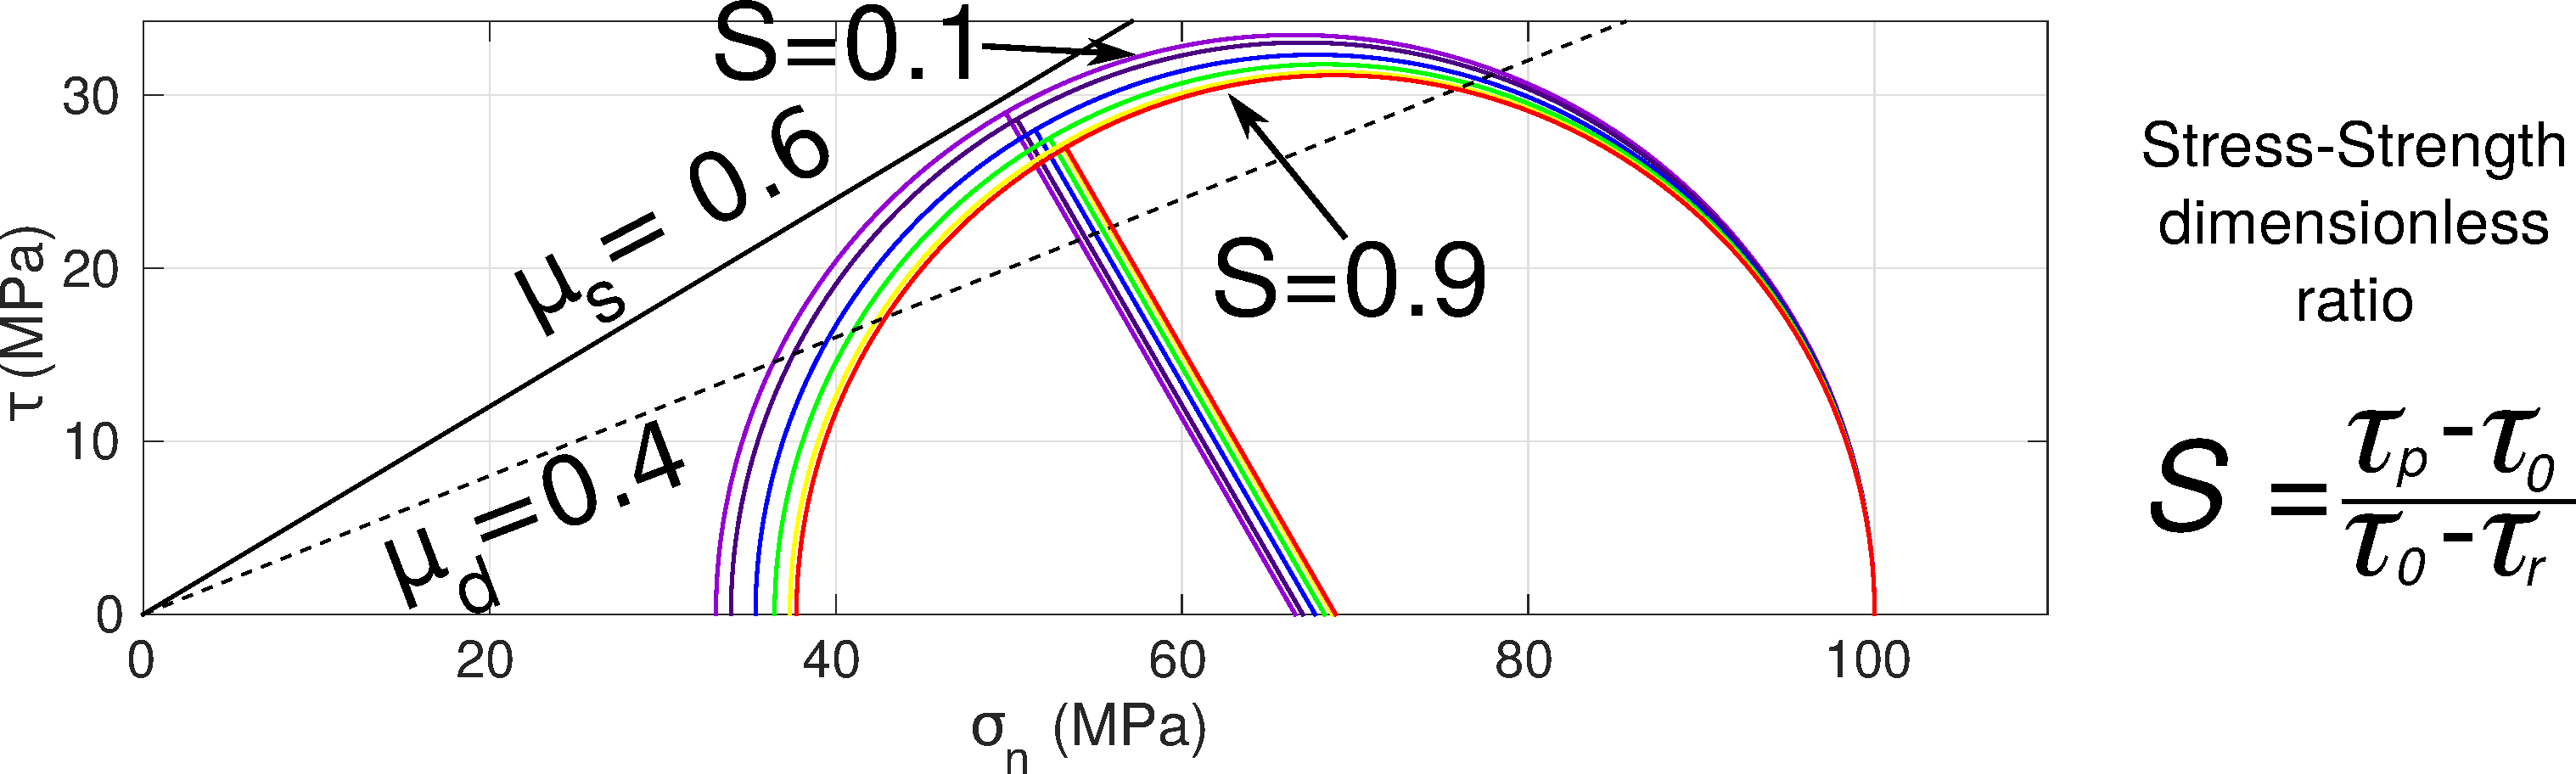
\includegraphics[width=0.9\linewidth]{images/MC_circle_2.pdf}
 \end{center}
  \centering \vskip -0.4cm Stress \& medium conditions \\
  \vskip 0.3cm
 \begin{minipage}{0.5\linewidth}
 \begin{itemize}
  \small \item \small Stress levels explored \\
  \small $S$ = 0.1, 0.2, 0.4, 0.6, 0.8, 0.9 \pause
  \vskip 0.2cm
  \item \small Linear Slip Weakening: $\mu_s$=0.6, 
  $\mu_d$=0.4, $d_c$=0.15 m \pause
  \vskip 0.2cm
  \item \small Slow rupture initiation \\ \hskip 0.5cm $\mu_s \xrightarrow[t \to 1] \ \mu_d$  \\ at a 4$\times$4 km$^2$ patch \pause
 \end{itemize}
 \end{minipage}
 \begin{minipage}{0.48\linewidth} \,
 \begin{itemize}
  \item \small $\sigma_{zz}$ depth-dependent \\ 
  {\tiny $\sigma_{zz} = (\rho - 1x10^3)*g*\min(-1.5x10^3, z)$}\pause
  \vskip 0.2cm
  \item \small Layered medium from Tinti et al. (2021) \pause
  \vskip 0.2cm
  \item \small Faults share same stress level
 \end{itemize}
 \end{minipage}

 \hfill {\tiny Inspired by \cite{Aochi_2018_DAN}}
 
\end{frame}


\begin{frame}
 {Preliminary exploration: 3 different cases}

 \begin{center}
 For these cases: Gap = 1 km, Offset = 1 km \\
 \vskip 0.4cm
 \begin{minipage}{0.45\linewidth}
    \centering \small Only 1 fault segment breaks \\
  	\animategraphics[autoplay,loop,width=\textwidth]{1}{images/nojump/nojump_neg_00}{00}{04}
    $S$: 0.6
 \end{minipage} \quad 
 \begin{minipage}{0.45\linewidth}
  \quad \hfill \quad
 \end{minipage} \\
 \begin{minipage}{0.45\linewidth}
  \quad \hfill \quad
  \end{minipage}
 \end{center}
 
\end{frame}


\begin{frame}
 {Preliminary exploration: 3 different cases}

 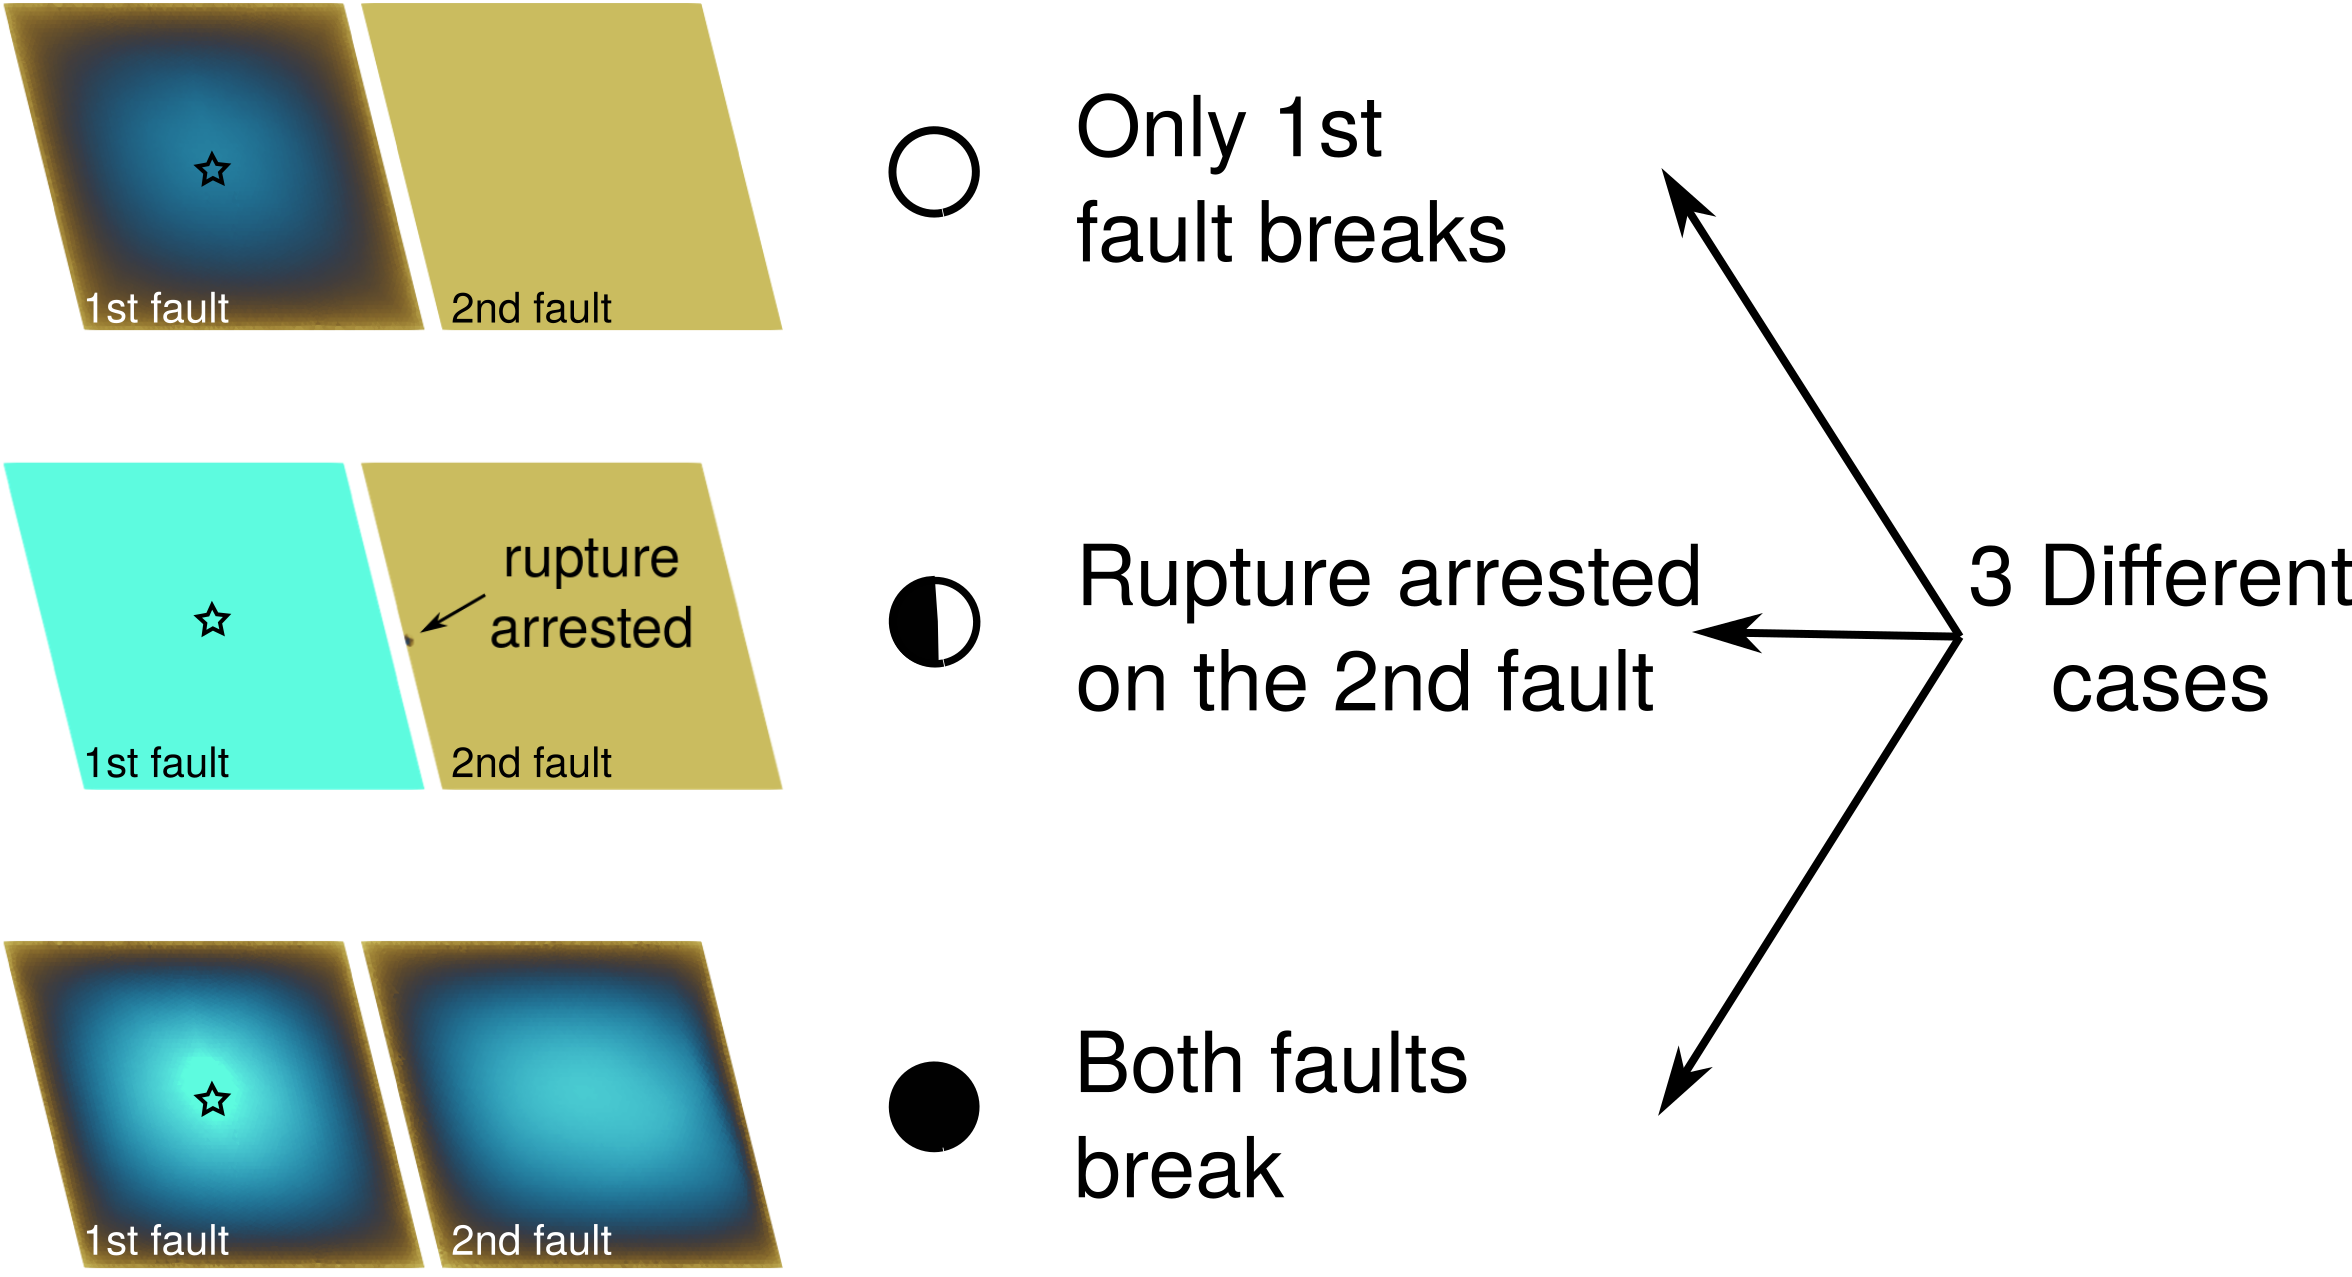
\includegraphics[width=1\linewidth]{images/cases.png}
 \addtocounter{framenumber}{-1}
 
\end{frame}



\begin{frame}
 {Preliminary exploration: Results from simulations}
 
{\small 72 simulations: [4] Gap values $\times$ [3] Offset values $\times$ [6] Stress levels}
 \vskip 0.2cm
 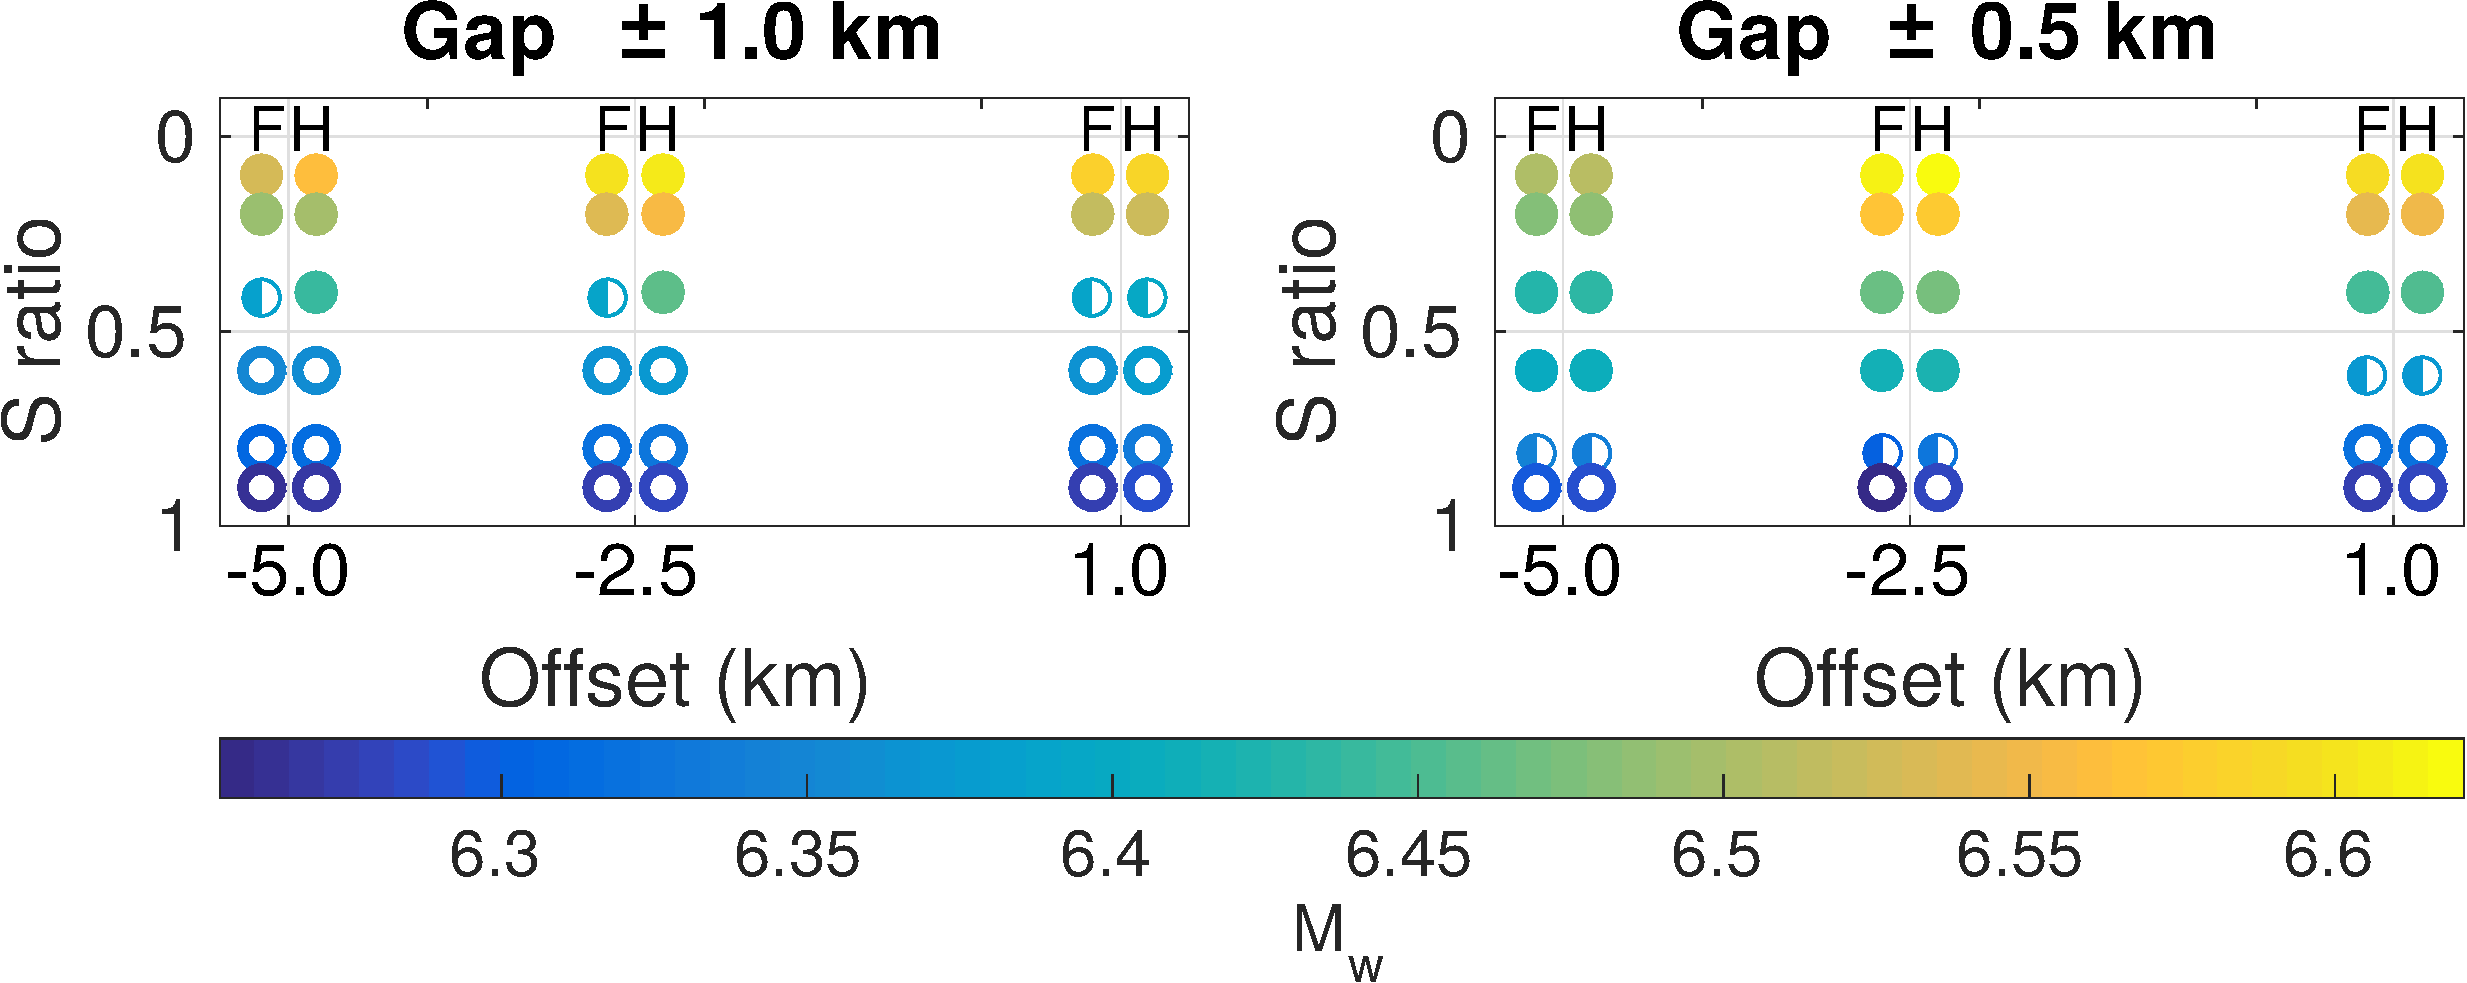
\includegraphics[width=1\linewidth]{images/results_table}
\vskip -0.5cm{\bf Under this configuration:} \pause \\
\vskip 0.1cm
\small $S$ depends only on the stress level and not on $\mu_s$ or $\mu_d$. \pause \\ 
\vskip 0.1cm
\small Rupture is arrested mainly due to the pre-stress level of faults. \pause \\
\vskip 0.1cm
\small Beyond $>1$ km offset jumps might be expected only at low $S$-ratio levels. \pause \\
\vskip 0.1cm
\small {\bf Stress shadow} and {\bf hanging/foot wall asymmetry} are observed. 

\end{frame}


\section{Preliminary conclusions \& discussion}

\begin{frame}
 {Hanging/foot wall behavioral asymmetry}
 
 \begin{center}
 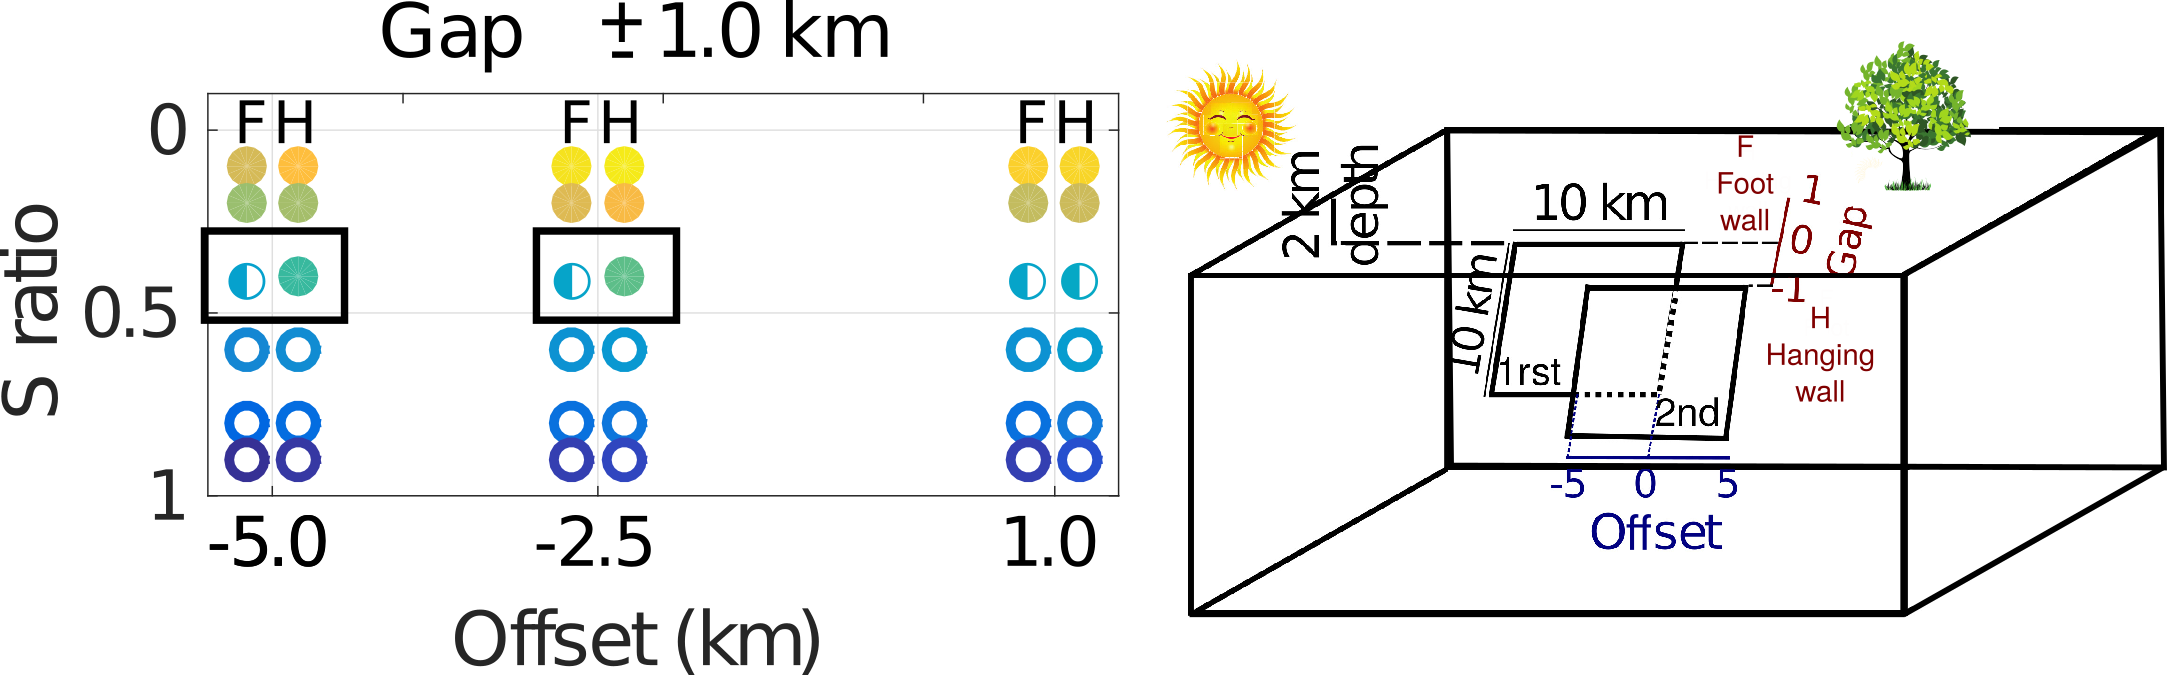
\includegraphics[width=1\linewidth]{images/schematic_view_noparam.png} 
 \end{center}

{\bf Triggering potential:}
\vskip 0.2cm
When the 2nd fault is located on the hanging wall (with respect to the 1st fault) the dynamically triggered rupture is more likely to be self-sustainable (break away).

\end{frame}



\begin{frame}
 {Stress shadow: Slip VS Fault Proximity}

\begin{center}
\vskip -0.2cm    \centering For these cases: Gap = 0.5 km, $S$ = 0.1 
\vskip 0.2cm 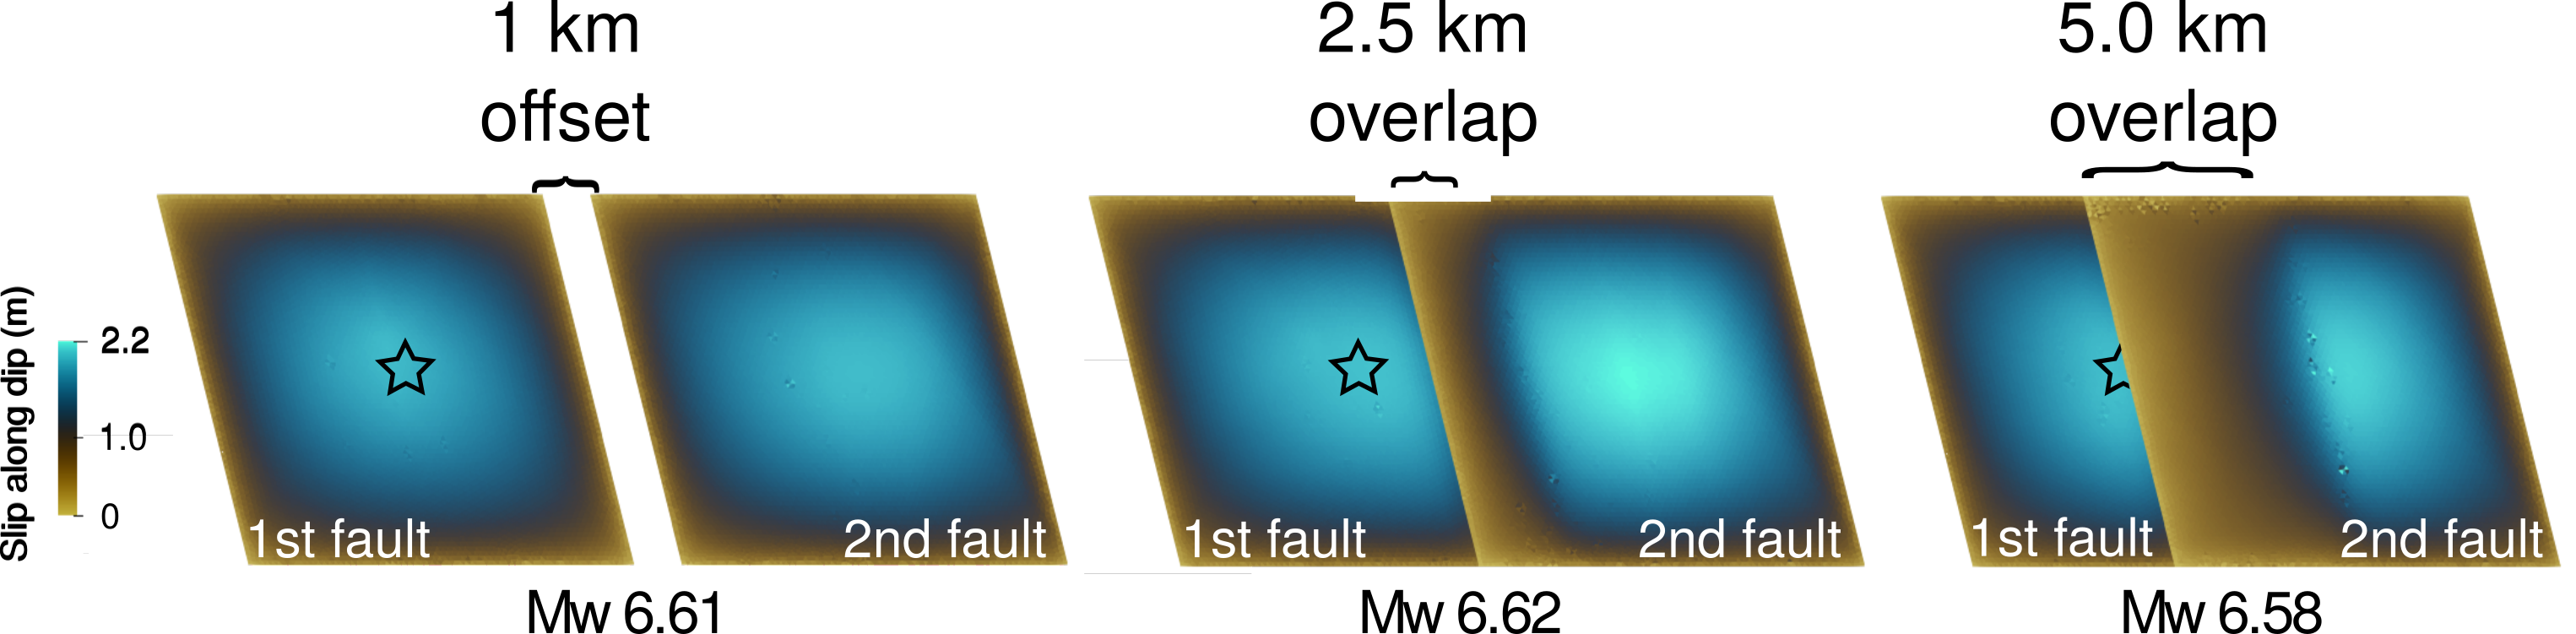
\includegraphics[width=1\linewidth]{images/stress_shadow.png}
\end{center}
\vskip -0.2cm
{\bf Slip VS Fault Proximity:}
\vskip 0cm
The final slip distribution (estimated energy) increases/decreases according to the distance between faults. 
\vskip -0.6cm \pause
\begin{equation*}
 \textnormal{Large overlap} \rightarrow \textnormal{Fault proximity} \rightarrow \textnormal{high triggering effect} 
\end{equation*}
\vskip -0.6cm
but, \pause
\vskip -0.8cm
\begin{equation*}
 \textnormal{Stress shadow} \rightarrow \textnormal{decreases slip distribution on 2nd fault}
\end{equation*}
 
\end{frame}


\section{On going work and to dos!}

\begin{frame}
  {Central Italy complex normal faulting system}

  \begin{minipage}{0.4\linewidth}
  \begin{center}
   \vskip 0.2cm Mapped fault traces \\
   \vskip 0.3cm
   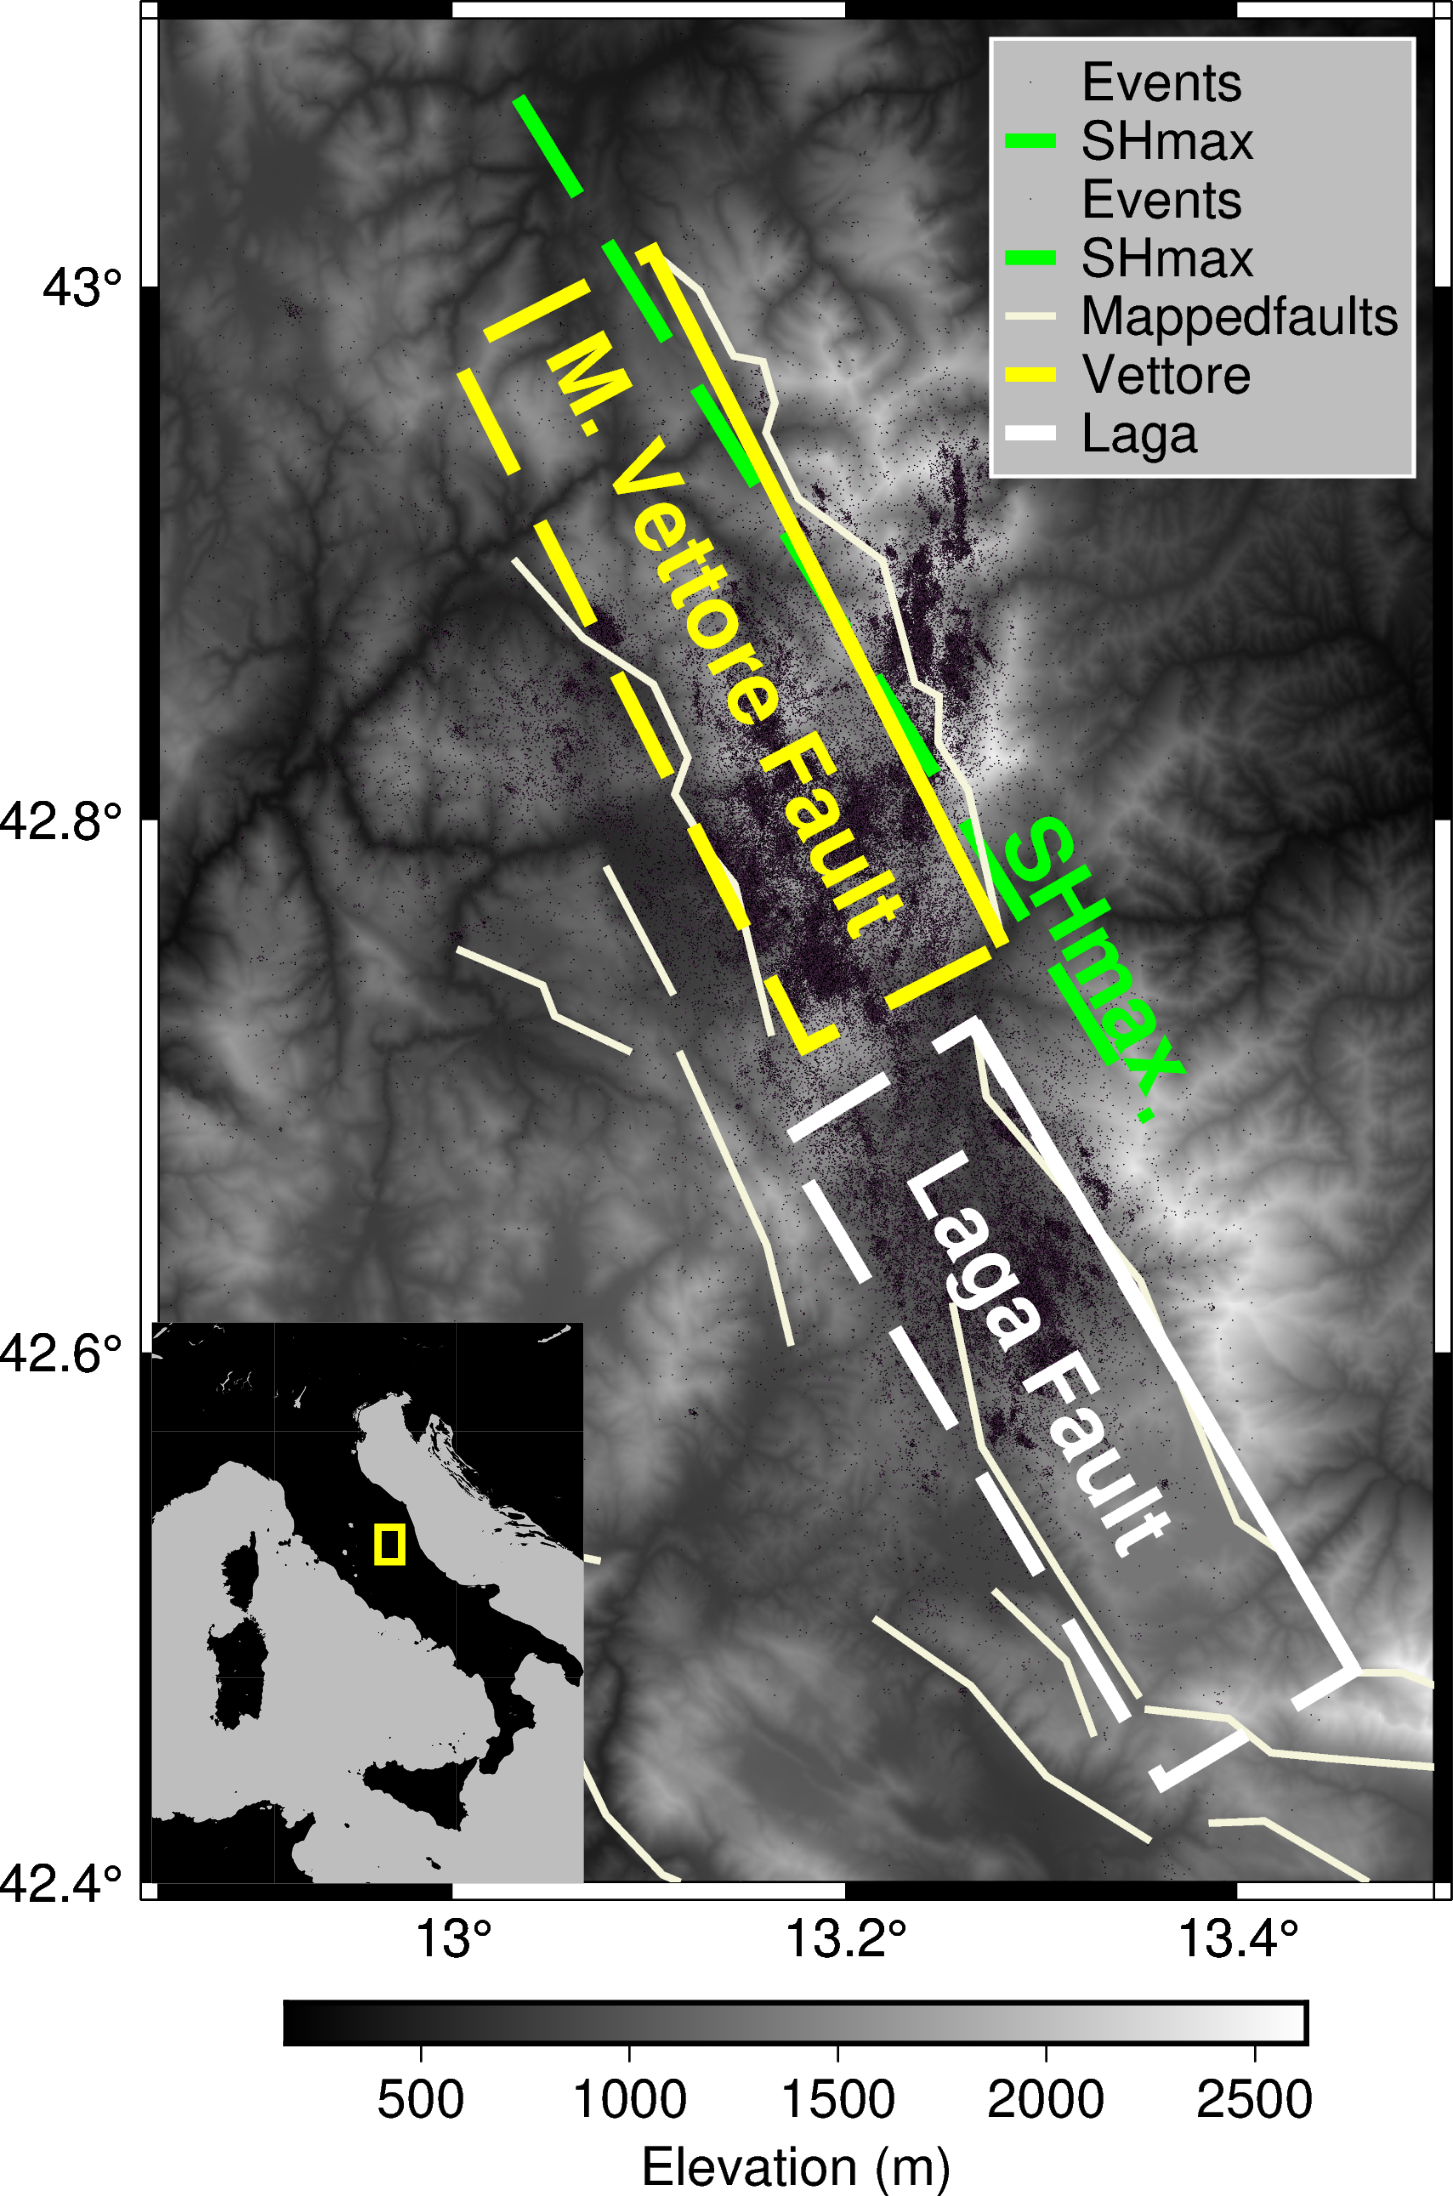
\includegraphics[width=1\linewidth]{images/map_italy.png}
  \end{center}
  \vskip -0.2cm \tiny Fault2SHA Database \citep{Walker_2021_FAULT2SHA}
 \end{minipage} \
 \begin{minipage}{0.57\linewidth}
  \begin{center}
   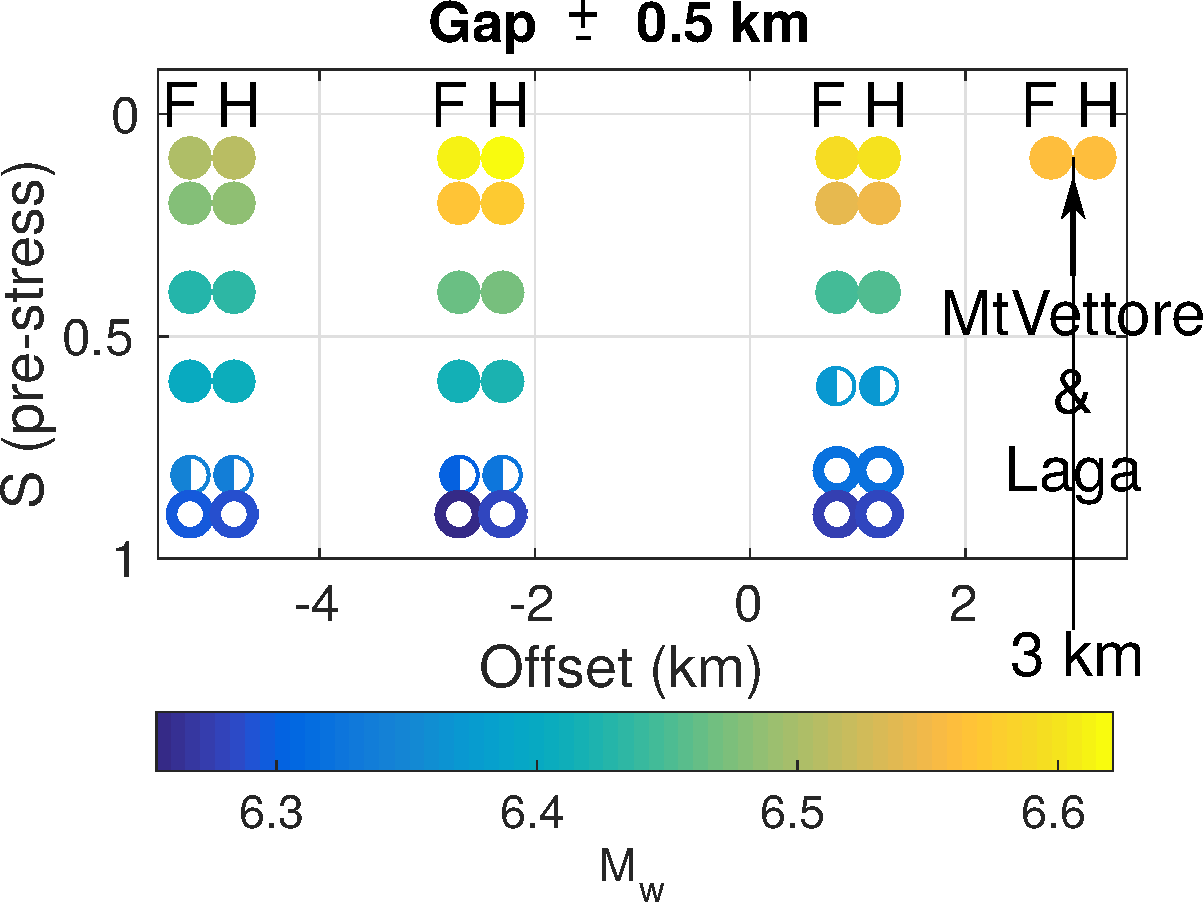
\includegraphics[width=0.9\linewidth]{images/linking}
  \end{center}  
 \vskip -0.5cm {\bf \footnotesize Central Italy:} \\
 \vskip -0.7cm
 \begin{itemize}
  \scriptsize \item[\ding{43}] \scriptsize Extensional regime
  \vskip 0.1cm
  \item[\ding{43}] \scriptsize Multi-segment normal faulting system
  \vskip 0.1cm
  \item[\ding{43}] \scriptsize Complex fault geometry
  \vskip -0.1cm
  \item[\ding{43}] \scriptsize Seismicity along one or serveral segments
   \begin{itemize}
   \item \scriptsize 1980 Ms6.9 Irpinia
   \item \scriptsize 2016 Amatrice-Visso-Norcia
   \end{itemize}
 \end{itemize}
 \end{minipage}
 
\end{frame}


\begin{frame}
 {Static or Dynamic triggered?}
 
 
 \begin{minipage}{0.45\linewidth}
 \begin{center}
  {\large Static Coulomb Stress Change} \\ 
  (1 fault only!)
 \end{center}
  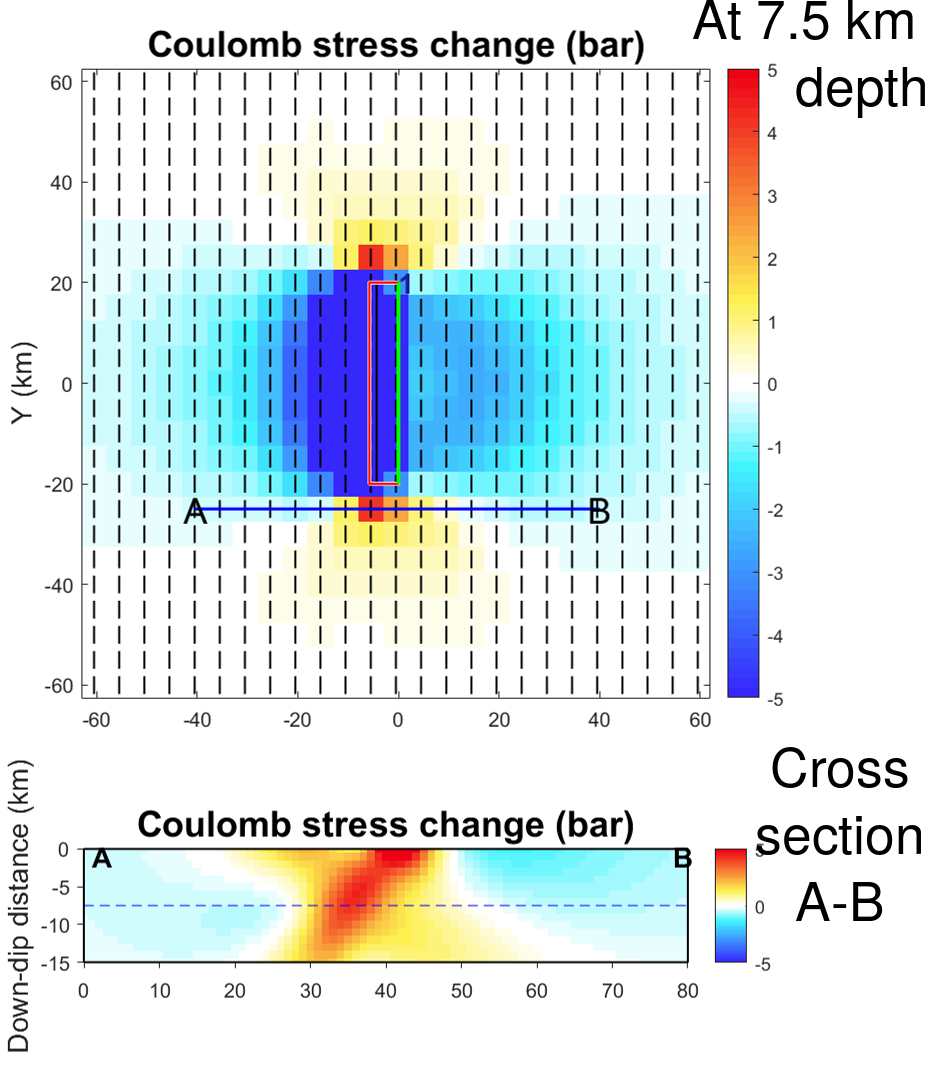
\includegraphics[width=1\linewidth]{images/CSC.png}
 \end{minipage}
 \begin{minipage}{0.45\linewidth}
 {\bf On going:}
  \begin{itemize}
   \item More simulations covering larger distances ($>$5 km)
   \\
   \item Estimation of dynamic stress changes
   \\
   \item Linking simulations with real case
   \\
   \item Writing results!
  \end{itemize}
 \end{minipage}

 
\end{frame}




\section*{References}
\begin{frame}nbn 

    {\tiny \bibliography{\dirbiblio/bibliography} }							\bibliographystyle{apalike}    

\end{frame}





\end{document}







 



\section{On going work and to dos!}



\begin{frame}
 {Things to do}
 
 Some steps to follow (little by little): \\
 \vskip 0.4cm \pause
 \begin{itemize}
  \item Complexify fault geometry, larger, rougher, ... \pause
  \vskip 0.4cm
  \item Account for a stratified embedding medium \pause
  \vskip 0.4cm
  \item More realistic stress field: regional, depth-dependent \pause
  \vskip 0.4cm
  \item Include topography
 \end{itemize}
\pause
\begin{center}
 \underline{\bf While exploring for the physical properties}\\
 \underline{\bf promoting rupture jumps across step overs} 
\end{center}
 
\end{frame}

\begin{frame}
 {Complexifying the fault geometry}
 
 \begin{minipage}{0.45\linewidth}
  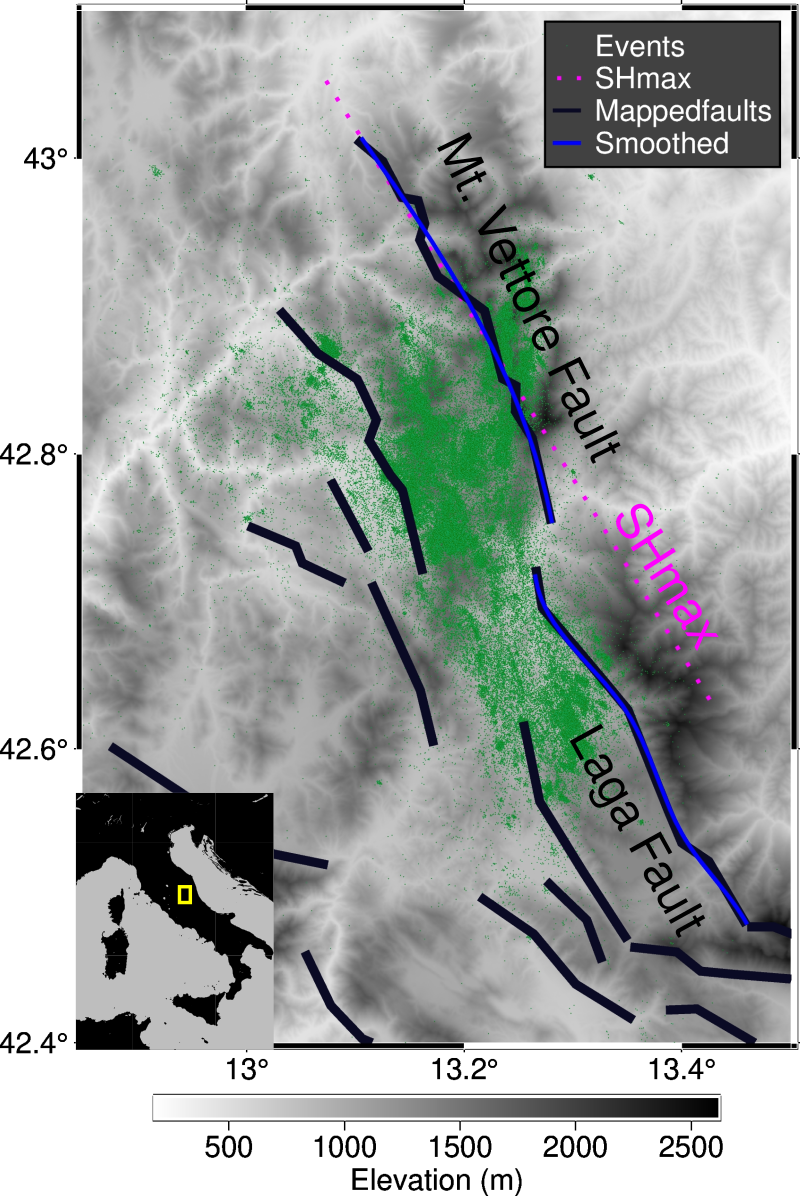
\includegraphics[width=1\linewidth]{images/faults.png}
  {\tiny Events from \cite{Tan_2021_MLB}}
 \end{minipage} \qquad \pause
 \begin{minipage}{0.45\linewidth}
  \includegraphics[width=1\linewidth]{images/faults_mesh_dip.png}
 \end{minipage}

\end{frame}


\begin{frame}
 {Initial exploration with complex geometry}
 
 \begin{minipage}{0.45\linewidth}
 \begin{center}
  {\bf Initial shear stress \\ along dip (Pa)}
  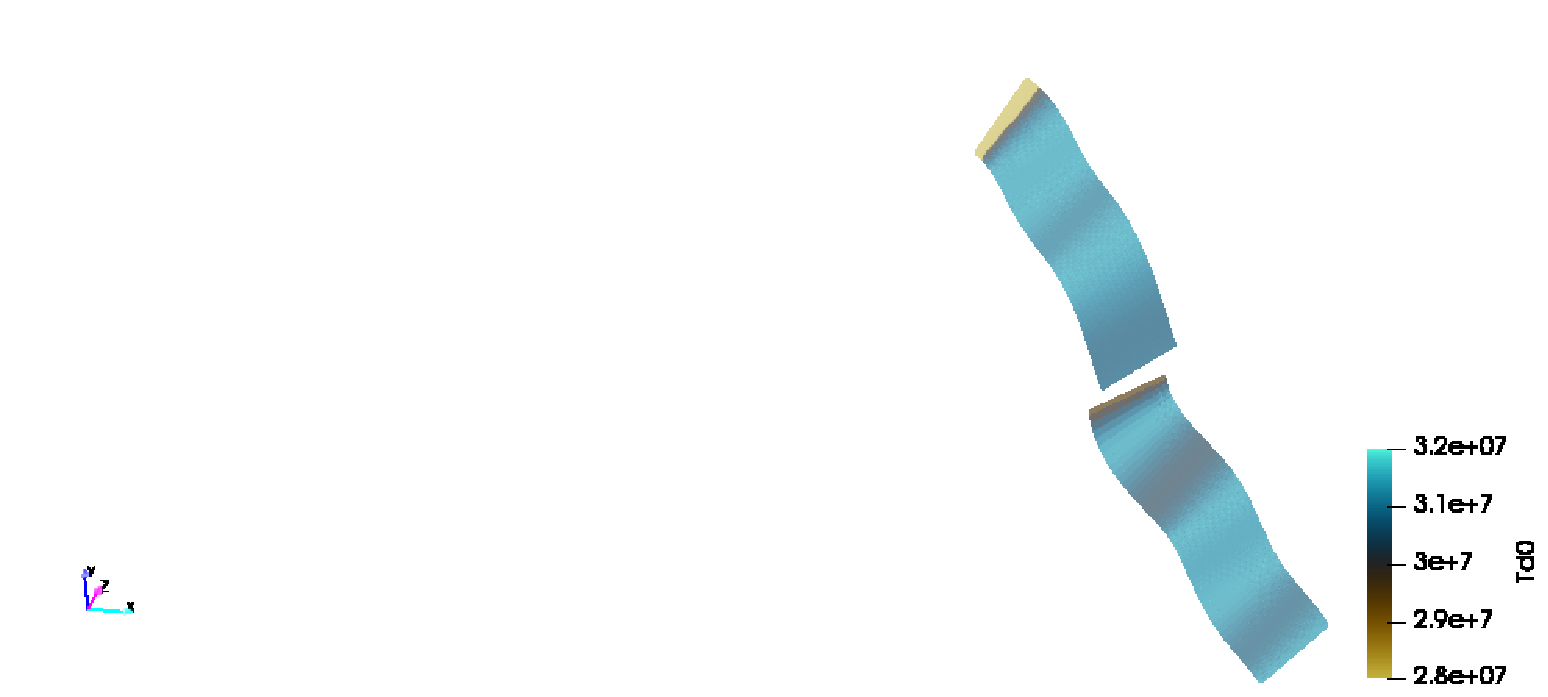
\includegraphics[width=1\textwidth]{images/Td0_neg.pdf}  
 \end{center}
 \end{minipage}
 \begin{minipage}{0.53\linewidth}
 {\bf Summary:}
 \vskip 0.3cm
 \begin{itemize}
  \small \item \small Stress levels explored $S$ = 0.1
  \vskip 0.3cm
  \item \small Linear Slip Weakening: $\mu_s$=0.6, 
  $\mu_d$=0.4, $d_c$=0.15
  \vskip 0.3cm
  \item \small Slow rupture initiation \\ $\mu_s \xrightarrow[t \to 1] \ \mu_d$ at $16\pi$ km$^2$ patch
  \vskip 0.3cm
  \item \small $\sigma_{zz}=100$ MPa ($\sim$3.6 km depth)
  \vskip 0.3cm
  \item \small Homogeneous half-space \\ \scriptsize $V_p$=6.3, $V_s$=3.6 $km/s$, $\rho$=2800 $kg/m^3$   \vskip 0.3cm
  \item \small Stress level affected by geometry \end{itemize}
 \end{minipage}

\end{frame}


\begin{frame}
 {Initial exploration with complex geometry}
 
 \begin{minipage}{0.45\linewidth}
 \begin{center}
  {\bf Cumulative slip \\ along dip (m)}
  \animategraphics[autoplay,loop,width=1\textwidth]{1}{images/animations/Sld/Sld_neg_00}{01}{21}  
 \end{center}
 \end{minipage}
 \begin{minipage}{0.45\linewidth}
 \begin{center}
 {\bf Slip rate \\ along dip (m/s)}
  \animategraphics[autoplay,loop,width=1\textwidth]{1}{images/animations/SRd/SRd_neg_00}{00}{20}
 \end{center}
 \end{minipage}
 
 \begin{center}
  $\sim$20 seconds of rupture
 \end{center}

 
\end{frame}


\begin{frame}
 {Initial exploration: complex geometry + layered medium}
 
 \begin{center}
  \includegraphics[width=1\linewidth]{images/new/s_neg_1.png}
 \end{center}
 
\end{frame}

\begin{frame}
 {Initial exploration: complex geometry + layered medium}
 
 \begin{center}
  \includegraphics[width=1\linewidth]{images/new/s_neg_2.png}
 \end{center}
  \addtocounter{framenumber}{-1}
 
\end{frame}

\begin{frame}
 {Initial exploration: complex geometry + layered medium}
 
 \begin{center}
  \includegraphics[width=1\linewidth]{images/new/s_neg_3.png}
 \end{center}
  \addtocounter{framenumber}{-1}
 
\end{frame}

\begin{frame}
 {Initial exploration: complex geometry + layered medium}
 
 \begin{center}
  \includegraphics[width=1\linewidth]{images/new/s_neg_4.png}
 \end{center}
  \addtocounter{framenumber}{-1}
 
\end{frame}


\begin{frame}
 {Initial exploration: complex geometry + layered medium}
 
 
 \begin{center}
 {\bf Slip rate along dip direction (m/s)}
  \animategraphics[autoplay,loop,width=0.8\textwidth]{1}{images/new/new/srd_neg_0}{00}{10}  

  {\bf Cumulative slip along dip direction (m)}
  \animategraphics[autoplay,loop,width=0.8\textwidth]{1}{images/new/new/s_test_neg_0}{00}{10}
  
 \scriptsize 20 sec. of simulation $\rightarrow$ 
  velocity model is the only change
  
 \end{center}
  
\end{frame}



\begin{frame}
 {Differences and to dos!}

 {\bf Differences compared to other studies:}
 \begin{itemize}
  \item \footnotesize We deal with normal faulting systems
  \item \footnotesize Under our configuration, beyond $>1$ km offset jumps might be expected only at low $S$-ratio levels
  \item \footnotesize Different ways to initiate the rupture
 \end{itemize}

 {\bf To dos:}
 \begin{itemize}
  \item \footnotesize Improve our mesh \Checkmark 
  \item \footnotesize Account for stratified media \Checkmark
  \item \footnotesize Explore depth-dependent and heterogeneous stress fields
  \item \footnotesize Include plasticity, topography, ...
 \end{itemize}
 
 \begin{center}
   \underline{\bf Thanks for listening!}  
 \end{center}

\end{frame}

\begin{frame}
 {Departure: From April 1 2022 CRCN IRD}
 
 \begin{itemize}
  \item Keep the exploration on this fault system \\
        Jan. -- Apr. : depth-dependent stress+topography+plasticity 
        \vskip 0.4cm
  \begin{itemize}
   \item Interact with the new postdoc (if there is a replacement) \\
         Apr. -- Jun.
  \end{itemize}
  \vskip 0.4cm
  \item Extend this research to other regions and fault systems
  \begin{itemize}
   \item Libanon (Dead Sea Fault), Peru ? \\
         Apr. -- Jul.
  \end{itemize}
  \vskip 0.4cm
  \item Prepare a publication related to this study \\
        Mar. -- \dots
  \vskip 0.4cm
  \item Prepare a report/tutorial of what I have done \\
        Mar. -- Apr.
 \end{itemize}

 
 
\end{frame}








\begin{frame}
 {Geological context}
 
 \begin{minipage}{0.5\linewidth}
 \vskip -0.5cm{\bf Central Italy:} \\
 \vskip 0.2cm
 \begin{itemize}
  \footnotesize \item[\ding{43}] \footnotesize Extensional regime
  \vskip 0.2cm
  \item[\ding{43}] \footnotesize Multi-segment normal faulting system
  \vskip 0.2cm
  \item[\ding{43}] \footnotesize Complex fault geometry
  \vskip 0.2cm
  \item[\ding{43}] \footnotesize Seismicity along one or serveral segments
   \begin{itemize}
   \item \footnotesize 1980 Ms6.9 Irpinia
   \item \footnotesize 2009 Mw6.1 L'Aquila
   \item \footnotesize 2016 Amatrice-Visso-Norcia
   \end{itemize}
 \end{itemize}

 \end{minipage}
 \begin{minipage}{0.45\linewidth}
 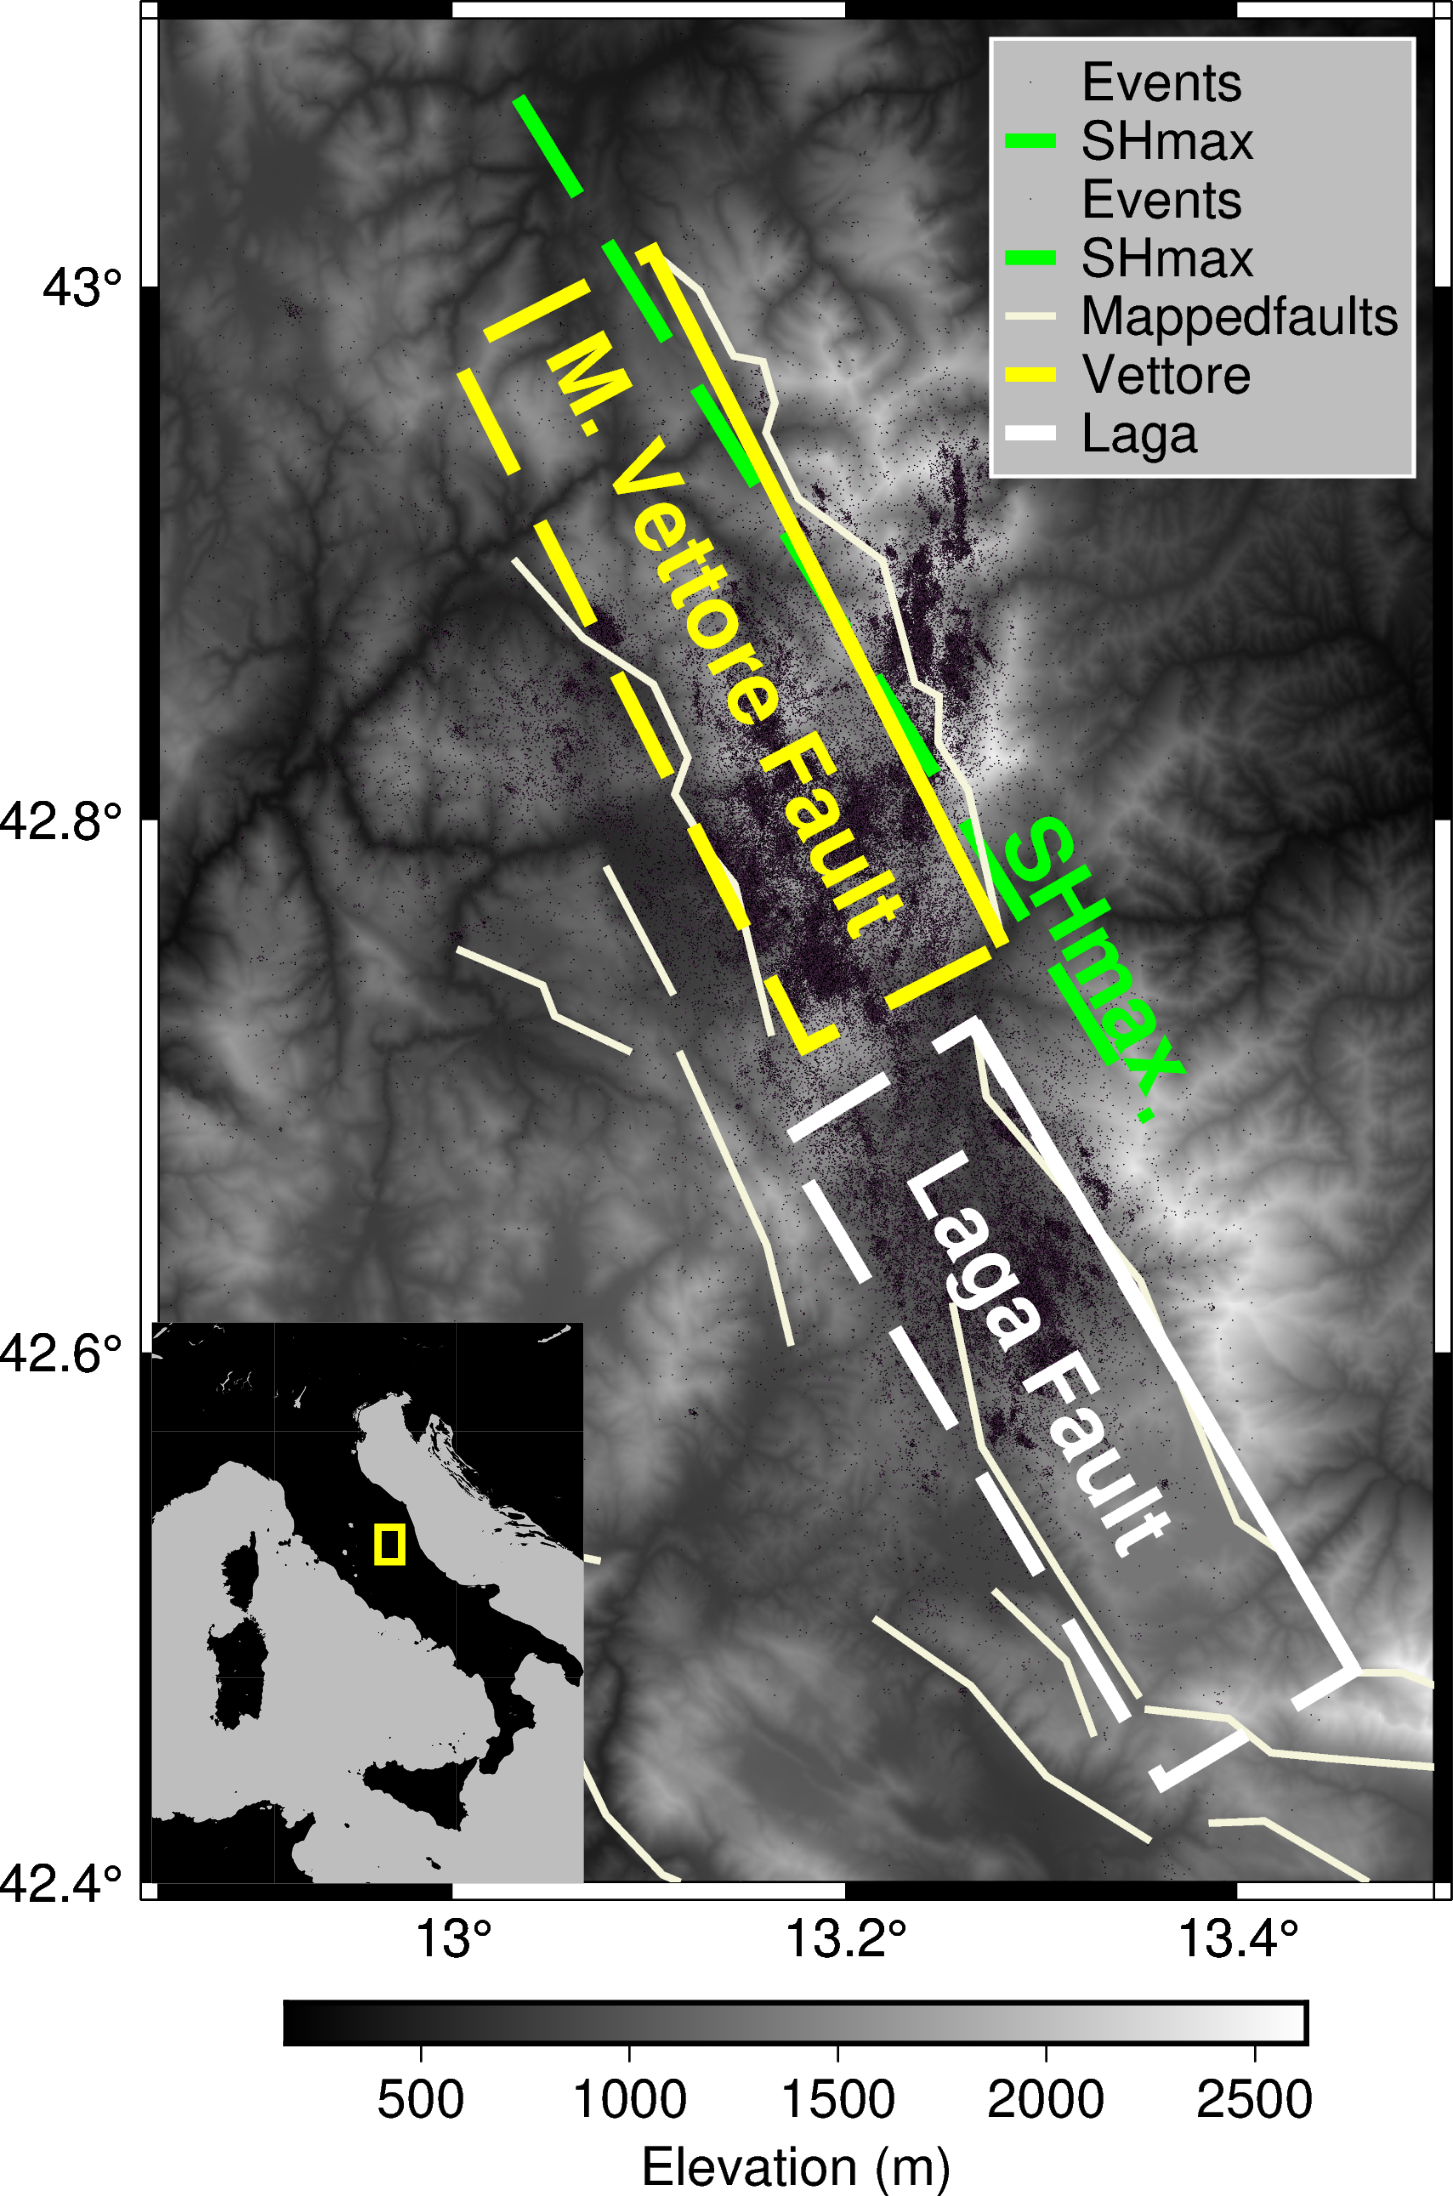
\includegraphics[width=1\linewidth]{images/map_italy}
 \end{minipage}

\end{frame}
